\documentclass[11pt]{article}
% preamble.tex -- house style of Gruppe Jahnel (TU Braunschweig)
\usepackage[T1]{fontenc}
\usepackage{lmodern}
\usepackage[utf8]{inputenc}
\usepackage[british]{babel}
\usepackage{amsmath,amssymb,amsthm,mathtools}
\usepackage[a4paper,margin=1.05in]{geometry}
\usepackage{microtype}
\setlength{\emergencystretch}{1em}
\usepackage{xcolor}
\definecolor{paperlink}{RGB}{0,0,114}
% shared figure colours (roles; every colour is paired with a line style or a label)
\definecolor{figmain}{RGB}{0,62,140}   % raw path, corridor, main objects
\definecolor{figaux}{RGB}{176,84,0}    % escapes, inserted pieces
\definecolor{figgrey}{gray}{0.5}       % guides, closed edges
\usepackage{enumitem}
\setlist[itemize]{leftmargin=2em,itemsep=0.25em,topsep=0.35em}
\setlist[enumerate]{leftmargin=2.25em,itemsep=0.25em,topsep=0.35em}
\usepackage{tikz}
\usetikzlibrary{arrows.meta,positioning,calc,decorations.pathmorphing,fit,backgrounds}
\usepackage{fancyhdr}
\pagestyle{fancy}
\fancyhf{}
\fancyhead[L]{\small Nonuniqueness on nonamenable transitive graphs}
\fancyhead[R]{\small\thepage}
\setlength{\headheight}{14pt}
\usepackage[hyphens]{url}
\usepackage{hyperref}
\hypersetup{colorlinks=true,linktoc=all,linkcolor=paperlink,citecolor=paperlink,
  urlcolor=paperlink,pdfstartview=Fit}
\usepackage[capitalise,nameinlink,noabbrev]{cleveref}
\setlength{\parindent}{1.25em}
\setlength{\parskip}{0pt}
\numberwithin{equation}{section}
\setcounter{tocdepth}{1}

% ---------------------------------------------------------------- theorems
\theoremstyle{plain}
\newtheorem{theorem}{Theorem}[section]
\newtheorem{proposition}[theorem]{Proposition}
\newtheorem{lemma}[theorem]{Lemma}
\newtheorem{corollary}[theorem]{Corollary}
\theoremstyle{definition}
\newtheorem{definition}[theorem]{Definition}
\newtheorem{assumption}[theorem]{Assumption}
\newtheorem{example}[theorem]{Example}
\theoremstyle{remark}
\newtheorem{remark}[theorem]{Remark}

% standing assumptions (A1), (A2): referenced with \cref
\newlist{asslist}{enumerate}{1}
\setlist[asslist]{label=\textup{(A\arabic*)},ref=\textup{(A\arabic*)},leftmargin=3em}
\crefformat{asslisti}{#2#1#3}
\Crefformat{asslisti}{#2#1#3}
\crefrangeformat{asslisti}{#3#1#4--#5#2#6}
\crefmultiformat{asslisti}{#2#1#3}{ and~#2#1#3}{, #2#1#3}{ and~#2#1#3}

% ---------------------------------------------------------------- macros
\newcommand{\PP}{\mathbb P}
\newcommand{\EE}{\mathbb E}
\newcommand{\N}{\mathbb N}
\newcommand{\Z}{\mathbb Z}
\newcommand{\R}{\mathbb R}
\DeclareMathOperator{\Var}{Var}
\DeclareMathOperator{\Cov}{Cov}
% indicator: \mathds 1 (dsfont); bold fallback where dsfont is not installed
\IfFileExists{dsfont.sty}{\usepackage{dsfont}\newcommand{\1}{\mathds{1}}}{\newcommand{\1}{\mathbf{1}}}
\newcommand{\e}{\mathrm{e}}
% \d and \c: upright d and complement sign in math mode, the usual accents in text mode
\let\accentdotbelow\d
\DeclareRobustCommand{\d}{\ifmmode\mathrm{d}\else\expandafter\accentdotbelow\fi}
\newcommand{\dd}{\,\mathrm{d}}
\let\accentcedilla\c
\DeclareRobustCommand{\c}{\ifmmode\mathrm{c}\else\expandafter\accentcedilla\fi}
\DeclarePairedDelimiter{\abs}{\lvert}{\rvert}
\DeclarePairedDelimiter{\norm}{\lVert}{\rVert}
\DeclareMathOperator{\tr}{tr}
\DeclareMathOperator{\Adj}{Adj}
\DeclareMathOperator{\dist}{dist}
\DeclareMathOperator{\diam}{diam}
\DeclareMathOperator{\Aut}{Aut}
\DeclareMathOperator{\Piv}{Piv}
\DeclareMathOperator{\Cay}{Cay}
\newcommand{\given}{\,\lvert\,}
\newcommand{\conn}{\leftrightarrow}
\newcommand{\nconn}{\mathrel{\not\leftrightarrow}}
\newcommand{\connin}[1]{\xleftrightarrow{\;#1\;}}
\newcommand{\ptwo}{p_{2\to 2}}
\newcommand{\pexp}{p_{\mathrm{exp}}}
\newcommand{\dbr}{d_{\mathrm{br}}}
\newcommand{\diambr}{\diam_{\mathrm{br}}}
\newcommand{\radbr}{\operatorname{rad}_{\mathrm{br}}}
\newcommand{\radint}{\operatorname{rad}_{\mathrm{int}}}
\newcommand{\radext}{\operatorname{rad}_{\mathrm{ext}}}
\newcommand{\Nb}{\mathrm{N}}                   % closed neighbourhood N[A]
\newcommand{\Cor}{\mathrm{Cor}}                % corridor event
\newcommand{\Bl}{\mathrm{Bl}}                  % blockers
\newcommand{\Erw}{\mathbf{E}^{\mathrm{rw}}_{k}}  % average over k-step lazy walk paths from o
\newcommand{\Ehat}{\widehat{\EE}}


\hypersetup{pdftitle={Nonuniqueness of percolation on nonamenable transitive graphs},
  pdfsubject={The Benjamini--Schramm nonuniqueness conjecture: the proof in the transitive case}}

\title{Nonuniqueness of percolation on nonamenable transitive graphs\\[0.4em]
  \large An account of the proof in the transitive case}
% TODO(Claude): the author line is a placeholder; to be settled by the user.
\author{Notes for a reading course\thanks{These notes rewrite,
  for transitive graphs, the proof given in the manuscript~\cite{Ope26}, where the quasi-transitive
  case is treated.}}
\date{}

\begin{document}
\maketitle

\begin{abstract}
We present, for transitive graphs, a proof that Bernoulli bond percolation on every connected,
locally finite, simple, nonamenable transitive graph has a phase with infinitely many infinite
clusters, that is, $p_c<p_u$. The argument is the one of~\cite{Ope26}, specialised and reorganised.
Its core is the statement that the two-point connection operator is bounded on $\ell^2(V)$ at the
critical parameter. Together with results of Hutchcroft this gives $p_c<\ptwo\le p_u$, where $\ptwo$ is
the largest parameter up to which the connection operator is bounded, a nonempty interval of
simultaneous nonuniqueness, the triangle condition and mean-field critical behaviour. The proof of
the operator bound compares two ways of measuring the connection kernel: its row sums and its norm on
$\ell^2(V)$. A deformation that penalises connections through isolated open paths reduces the row
sums at a quadratic rate while barely changing the norm, because the penalised paths are
loop-erased random-walk paths and the random walk contracts $\ell^2(V)$. Making this quantitative
needs near-mean-field a priori bounds on the susceptibility and the triangle diagram below $p_c$.
These are derived from finiteness of all moments of order less than $1/2$ of the critical cluster
size, which in turn is proved by contradiction with a construction that splices independent
critical clusters. We decompose the argument into four steps, state each step precisely, and show
how the steps combine before proving them.
\end{abstract}
\clearpage

\tableofcontents
\clearpage

\section{Introduction}\label{sec:intro}

In Bernoulli bond percolation with parameter $p\in[0,1]$ on an infinite connected graph, every edge is
declared open with probability~$p$, independently of all other edges, and one studies the connected
components of the open subgraph, the \emph{clusters}. Two parameters describe the large-scale picture.
Infinite clusters exist for $p$ above the \emph{critical parameter}~$p_c$, and there is exactly one
infinite cluster for $p$ above the \emph{uniqueness threshold}~$p_u$. On the hypercubic lattice
$\Z^d$ there is never more than one infinite cluster~\cite{AKN87,BK89}, and the argument of Burton and
Keane extends this to every amenable transitive graph (see~\cite[Chapter~7]{LP16}); there the two
thresholds coincide. On the $3$-regular tree, in contrast, $p_c=1/2$ and $p_u=1$: for every
$p\in(1/2,1)$ there are infinitely many infinite clusters, kept apart by the branching geometry of the
tree. Benjamini and Schramm conjectured that the thresholds are separated on every quasi-transitive
graph that shares the decisive feature of the tree, namely that the boundary of every finite vertex
set is comparable to its size~\cite[Conjecture~6]{BS96}. Such graphs are called nonamenable.

These notes present a proof of this conjecture for transitive graphs, following the
manuscript~\cite{Ope26}. In informal terms, the main result reads as follows; the precise statement is
\cref{thm:main}.

\begin{quote}
\emph{Let $G$ be a connected, locally finite, simple, nonamenable transitive graph. Then the matrix of
connection probabilities at the critical parameter defines a bounded operator on $\ell^2(V)$.
Consequently $p_c<\ptwo\le p_u$, so there is a nonempty interval of parameters with infinitely many
infinite clusters, and percolation on $G$ has mean-field critical behaviour.}
\end{quote}

Here $\ptwo$ is the largest parameter up to which the connection probabilities define a bounded
operator on $\ell^2(V)$. This threshold was introduced by Hutchcroft~\cite{Hut19,Hut20L2}, who
conjectured that $p_c<\ptwo$ on every nonamenable quasi-transitive graph~\cite[Conjecture~1.3]{Hut20L2}.
The inequality $\ptwo\le p_u$ is elementary: a unique infinite cluster forces all connection
probabilities to be bounded away from zero, which is incompatible with boundedness on $\ell^2(V)$
(\cref{lem:p22-pu}). The strict inequality $p_c<\ptwo$ is the substance of the result. It follows from
boundedness at $p_c$ itself, because a bounded connection operator remains bounded after a small
increase of the parameter (\cref{lem:sprinkling}).

\paragraph{Earlier results.}
Several classes of graphs were known to satisfy $p_c<p_u$. Benjamini and Schramm proved it for
one-ended nonamenable transitive planar graphs~\cite{BS01}, following Lalley's work on Fuchsian
groups~\cite{Lal98}. Schonmann treated highly nonamenable graphs~\cite{Sch01}, and Nachmias and Peres
nonamenable Cayley graphs of large girth~\cite{NP12}. Gaboriau proved $p_c<p_u$ for unimodular
transitive graphs carrying nonconstant harmonic Dirichlet functions~\cite{Gab05}. For Cayley graphs of
a given nonamenable group, Pak and Smirnova-Nagnibeda~\cite{PSN00} and Thom~\cite{Tho15} showed that
\emph{some} generating set has $p_c<p_u$; the result presented here applies to \emph{every} finite
generating set (\cref{cor:cayley}). In the operator framework, Hutchcroft proved $p_c<\ptwo$ for
nonamenable Gromov hyperbolic graphs and for graphs with a quasi-transitive nonunimodular group of
automorphisms~\cite{Hut19}, building on~\cite{Hut20nonuni}. Choi and Seo extended this to Cayley graphs
of acylindrically hyperbolic groups~\cite{CS25}. The upper inequality $\ptwo\le p_u$ can be an
equality~\cite{HP24}.

Critical percolation on a nonamenable transitive graph has no infinite cluster: this was proved by
Benjamini, Lyons, Peres and Schramm in the unimodular case~\cite{BLPS99a} and by Hutchcroft for all
quasi-transitive graphs of exponential growth~\cite{Hut16}. We use it throughout, since it makes
critical clusters finite. The behaviour of infinite clusters for $p_c<p<p_u$, including the
simultaneous statements across parameters, was developed by H\"aggstr\"om, Peres and
Schonmann~\cite{HP99,Sch99,HPS99}.

\paragraph{Methods.}
The proof uses the classical toolbox of percolation: the Harris and van den Berg--Kesten
inequalities~\cite{Har60,vdBK85}, the tree-graph bounds of Aizenman and Newman~\cite{AN84}, sharpness of
the phase transition~\cite{AB87,Men86,DCT16}, Russo's formula, and the mass-transport
principle~\cite{BLPS99b,AL07}. Two further tools enter in an essential way. The first is the
decision-tree covariance inequality of O'Donnell, Saks, Schramm and Servedio~\cite{OSSS05}, used as in
Hutchcroft's derivation of near-critical bounds from critical tails~\cite{Hut20exp}. The second is a
concentration estimate for exploration scores in the spirit of Hutchcroft's two-ghost
inequalities~\cite{Hut20loc,Hut21}. The genuinely new ingredients of~\cite{Ope26} are a construction
that splices independent critical clusters together (\cref{sec:maps}), whose combinatorics is related
to the finite modifications in Kozma's work on products of trees~\cite{Koz11}, and a deformation of the
connection kernel that penalises isolated open paths (\cref{sec:deformation}).

\paragraph{About these notes.}
The manuscript~\cite{Ope26} treats quasi-transitive graphs, possibly with loops and multiple edges.
We restrict to transitive simple graphs, which removes the averaging over vertex types, the reduction
to simple graphs by subdivision and several case distinctions, and lets the main line of the argument
stand out. The mathematics is that of~\cite{Ope26}; we have re-derived every step while rewriting it,
specialised the statements to the transitive case, and reorganised the material around four steps
whose precise statements are collected in \cref{sec:strategy}. Where a proof deviates from~\cite{Ope26}
beyond this specialisation, we say so. Classical results are cited rather than reproved; proofs are
given for the less standard variants we need, some of them in \cref{app:aux}.

\paragraph{Outline.}
\Cref{sec:setting} fixes the setting and states the main results:
\cref{thm:main}, its consequence for Cayley graphs, and the mean-field consequences in
\cref{thm:consequences}. \Cref{sec:strategy} is an overview of the whole proof. It reduces
\cref{thm:main} to the boundedness of the critical connection operator (\cref{thm:crit-bdd}), explains
the mechanism, states the four steps precisely, and proves \cref{thm:crit-bdd} from them.
\Cref{sec:prelim} collects the tools. \Cref{sec:bridges,sec:maps,sec:moments,sec:triangle} prove the a
priori estimates on critical and near-critical clusters (Steps~1 and~2), and
\cref{sec:deformation,sec:escapes} the properties of the deformation (Steps~3 and~4).
\Cref{sec:consequences} derives \cref{thm:consequences}.

\section{Setting and main results}\label{sec:setting}

\subsection{Graphs and standing assumptions}\label{sec:graphs}

Let $G=(V,E)$ be a graph with vertex set $V$ and edge set $E$. We write $x\sim y$ if $\{x,y\}\in E$,
$\dist$ for the graph distance, $B(x,r)$ for the closed ball of radius~$r$ around~$x$, and
$\Aut(G)$ for the group of graph automorphisms. For $A\subseteq V$ let $\partial_E A$ be the set of
edges with exactly one endpoint in~$A$, and let $\Nb[A]$ be the closed neighbourhood of~$A$, consisting
of $A$ and all vertices adjacent to a vertex of~$A$. The graph is \emph{transitive} if $\Aut(G)$ acts
transitively on~$V$, and \emph{nonamenable} if
\begin{equation*}
  \iota \coloneqq \inf\Bigl\{\frac{\abs{\partial_E A}}{\abs{A}} \colon A\subseteq V \text{ finite},\ A\neq\emptyset\Bigr\} > 0\,.
\end{equation*}
For graphs of bounded degree this is equivalent to positivity of the vertex-isoperimetric constant,
because every vertex of the outer vertex boundary of~$A$ is incident to at least one and at most
boundedly many edges of~$\partial_E A$.

Throughout these notes $G$ satisfies the following standing assumption.

\begin{asslist}
  \item\label{ass:G} $G=(V,E)$ is an infinite, connected, locally finite, simple graph, $\Aut(G)$ acts
  transitively on~$V$, and $G$ is nonamenable.
\end{asslist}

\noindent A transitive graph is regular; we write $d$ for its degree and fix a root vertex $o\in V$.
From \cref{sec:strategy} on, the main argument also uses the second assumption
\begin{asslist}[resume]
  \item\label{ass:U} the group $\Aut(G)$ is unimodular,
\end{asslist}
\noindent that is, $\abs{\operatorname{Stab}(x)y}=\abs{\operatorname{Stab}(y)x}$ for all $x,y\in V$, where
$\operatorname{Stab}(x)y$ is the orbit of $y$ under the stabiliser of~$x$ in $\Aut(G)$. Equivalently, the
mass-transport principle holds (\cref{sec:mtp}); every Cayley graph satisfies \cref{ass:U}. The
nonunimodular case is covered by a theorem of Hutchcroft (\cref{prop:nonunimodular}).

\subsection{Percolation, connection kernel and thresholds}\label{sec:percolation}

Let $\PP_p$ be the law of Bernoulli bond percolation with parameter $p\in[0,1]$ on~$G$, that is, the
product measure on $\{0,1\}^E$ under which each edge is \emph{open} ($\omega(e)=1$) with
probability~$p$, and let $\EE_p$ be its expectation. We write $x\conn y$ if $x$ and $y$ are joined
by an open path; paths of length zero are allowed, so $x\conn x$. The \emph{cluster} $C_x$ of~$x$ is
the set of vertices $y$ with $x\conn y$, and $\abs{C_x}$ is its number of vertices. For a vertex set
$\Lambda\subseteq V$, a \emph{domain}, we write $x\connin{\Lambda}y$ if $x$ and $y$ are joined by an open
path using only vertices of~$\Lambda$, and $C_x^\Lambda$ for the cluster of~$x$ in the subgraph induced
by~$\Lambda$. By convention $C_x^\Lambda=\emptyset$ if $x\notin\Lambda$, and every quantity that
requires a terminal outside its domain is zero. Let
\begin{equation*}
  \theta(p)\coloneqq\PP_p(\abs{C_o}=\infty)\,,\qquad
  p_c\coloneqq\inf\{p\colon\theta(p)>0\}\,,\qquad
  p_u\coloneqq\inf\{p\colon\PP_p(N_\infty=1)=1\}\,,
\end{equation*}
where $p$ ranges over $[0,1]$ and $N_\infty$ is the number of infinite clusters. In the \emph{standard monotone coupling} the
edges carry independent labels $U_e$ uniform on $[0,1]$, and an edge is open at parameter~$p$ if
$U_e\le p$; this realises all~$\PP_p$ on one probability space.

\paragraph{The connection kernel.}
A \emph{kernel} is a function $K\colon V\times V\to\R$. It is \emph{invariant} if $K(gx,gy)=K(x,y)$
for all $g\in\Aut(G)$ and $x,y\in V$. We let a kernel act on finitely supported functions by
$(Kf)(x)\coloneqq\sum_yK(x,y)f(y)$ and write $\norm{K}\in[0,\infty]$ for its operator norm on
$\ell^2(V)$, the Hilbert space of square-summable functions on~$V$ with counting measure; $K$ is
\emph{bounded} if $\norm{K}<\infty$. Products of nonnegative kernels,
$(KL)(x,y)\coloneqq\sum_zK(x,z)L(z,y)\in[0,\infty]$, are always defined. We write $\Adj$ for the
adjacency kernel, $\Adj(x,y)\coloneqq\1\{x\sim y\}$, and $I$ for the identity. The \emph{connection
kernel} and the \emph{operator threshold} are
\begin{equation*}
  T_p(x,y)\coloneqq\PP_p(x\conn y)\,,\qquad
  \ptwo\coloneqq\sup\{p\in[0,1]\colon \norm{T_p}<\infty\}\,.
\end{equation*}
More generally $T_p^\Lambda(x,y)\coloneqq\PP_p(x\connin{\Lambda}y)$. The \emph{susceptibility} and the
\emph{triangle diagram} are
\begin{equation*}
  \chi(p)\coloneqq\EE_p\abs{C_o}=\sum_{y\in V}T_p(o,y)\,,\qquad
  \nabla_p\coloneqq\sum_{y,z\in V}T_p(o,y)\,T_p(y,z)\,T_p(z,o)\,,
\end{equation*}
both with values in $[1,\infty]$. By transitivity they do not depend on the choice of~$o$.

\paragraph{Constants.}
Unless indicated otherwise, $c,C\in(0,\infty)$ denote constants that depend only on~$G$; their values
may change from line to line. Dependence on further parameters is shown by subscripts, as in~$C_\eta$.

\subsection{Main results}\label{sec:main-results}

\begin{theorem}[Critical boundedness and nonuniqueness]\label{thm:main}
Assume~\cref{ass:G}. Then
\begin{equation}\label{eq:main}
  \sup_{0\le p<p_c}\norm{T_p}=\norm{T_{p_c}}<\infty
  \qquad\text{and}\qquad
  p_c<\ptwo\le p_u\,.
\end{equation}
Moreover there are $p_c<p_1<p_2<1$ such that, in the standard monotone coupling, almost surely for
every $p\in[p_1,p_2]$ the open subgraph at parameter~$p$ has infinitely many infinite clusters.
\end{theorem}

The strict inequality $p_c<p_u$ is the bond-percolation case of the conjecture of Benjamini and
Schramm for transitive graphs.

\begin{corollary}[Cayley graphs]\label{cor:cayley}
Let $\Gamma$ be a finitely generated nonamenable group and $S\subseteq\Gamma$ a finite symmetric
generating set not containing the identity. Then the Cayley graph $\Cay(\Gamma,S)$, with vertex set
$\Gamma$ and edges $\{x,xs\}$ for $x\in\Gamma$ and $s\in S$, satisfies the conclusions of
\cref{thm:main,thm:consequences}.
\end{corollary}

\begin{proof}
The Cayley graph is simple, because the identity is not in~$S$ and edges are unordered pairs. It is
connected because $S$ generates~$\Gamma$, and locally finite because $S$ is finite. Left
multiplications are automorphisms, so it is transitive. By F{\o}lner's criterion a finitely generated
group is nonamenable if and only if one, equivalently every, of its Cayley graphs with respect to a
finite generating set is nonamenable (see~\cite[Chapter~6]{LP16}). % TODO: Referenz prüfen (exact locator in LP16)
Hence \cref{ass:G} holds, and \cref{thm:main,thm:consequences} apply.
\end{proof}

The operator bound also determines the critical behaviour. For a vertex $v$, the \emph{extrinsic} and
\emph{intrinsic radius} of its cluster are
\begin{equation*}
  \radext(C_v)\coloneqq\sup_{x\in C_v}\dist(v,x)\,,\qquad
  \radint(C_v)\coloneqq\sup_{x\in C_v}\dist_\omega(v,x)\,,
\end{equation*}
with values in $[0,\infty]$, where $\dist_\omega$ is the graph distance in the open subgraph. We say
that connection probabilities \emph{decay exponentially} at~$p$ if there are $A<\infty$ and $a>0$ with
$T_p(x,y)\le A\e^{-a\dist(x,y)}$ for all $x,y\in V$, and we let $\pexp$ be the supremum of all such~$p$.
We write $f\asymp g$ in a stated limit if $cg\le f\le Cg$ in a neighbourhood of that limit.

\begin{theorem}[Mean-field behaviour and exponential connectivity]\label{thm:consequences}
Assume~\cref{ass:G}. Then
\begin{equation}\label{eq:triangle-condition}
  \nabla_{p_c}\le\norm{T_{p_c}}^3<\infty\,,
\end{equation}
and, as $p\uparrow p_c$, $p\downarrow p_c$ and $n\to\infty$ respectively,
\begin{align}
  \chi(p)&\asymp(p_c-p)^{-1}\,,&
  \theta(p)&\asymp p-p_c\,,\label{eq:chi-theta}\\
  \PP_{p_c}(\abs{C_o}\ge n)&\asymp n^{-1/2}\,,&
  \PP_{p_c}\bigl(\radint(C_o)\ge n\bigr)\asymp\PP_{p_c}\bigl(\radext(C_o)\ge n\bigr)&\asymp n^{-1}\,.
  \label{eq:critical-tails}
\end{align}
Moreover $p_c<\ptwo\le\pexp$, and for every $p\in[0,\ptwo)$ there are $A_p<\infty$ and $a_p>0$ with
\begin{equation}\label{eq:exp-decay}
  T_p(x,y)\le A_p\,\e^{-a_p\dist(x,y)}\qquad\text{for all }x,y\in V\,.
\end{equation}
\end{theorem}

The bound~\eqref{eq:triangle-condition} is the \emph{triangle condition} of Aizenman and
Newman~\cite{AN84}. Together with $p_c<\pexp$ it verifies Conjectures~1.2 and~2.1 of~\cite{Hut20L2} for
transitive graphs. The asymptotics~\eqref{eq:chi-theta} and~\eqref{eq:critical-tails} are the
mean-field values of the critical exponents. They follow from known conditional results, whose
hypothesis is either the triangle condition or $p_c<\ptwo$; the new input is that these hypotheses hold
for every graph satisfying~\cref{ass:G}. The deduction is given in \cref{sec:consequences}.

\begin{remark}[Fixed parameters]\label{rem:fixed-p}
For each fixed $p\in(p_c,p_u)$ there are almost surely infinitely many infinite clusters. Indeed, on a
transitive graph $N_\infty$ is almost surely constant and belongs to $\{0,1,\infty\}$~\cite{NS81}
(see also~\cite[Chapter~7]{LP16}); it is positive because $p>p_c$, and it is not one because
$\PP_p(N_\infty=1)<1$ for $p<p_u$ by the definition of~$p_u$. H\"aggstr\"om, Peres and Schonmann proved
the stronger statement that this holds simultaneously for all $p\in(p_c,p_u)$ in the standard
coupling~\cite{HPS99}. The compact interval in \cref{thm:main} is obtained directly from the
boundedness of a single connection operator (\cref{prop:interval}).
\end{remark}

\begin{remark}[Scope]\label{rem:scope}
The manuscript~\cite{Ope26} treats quasi-transitive graphs, in which $\Aut(G)$ has finitely many
orbits, and also allows loops and multiple edges. A transitive graph with multiple edges does not
reduce to a transitive simple graph: subdividing each edge, as in~\cite{Ope26}, produces a simple
graph with two vertex orbits. Such graphs are therefore not covered by these notes.
\end{remark}

\section{Strategy of the proof}\label{sec:strategy}

The proof of \cref{thm:main} has two layers. The first is a short reduction to the boundedness of the
critical connection operator for graphs with a unimodular automorphism group
(\cref{sec:reduction}). The second proves this boundedness; it occupies
\cref{sec:prelim,sec:bridges,sec:maps,sec:moments,sec:triangle,sec:deformation,sec:escapes}. We first
explain the mechanism (\cref{sec:mechanism}). We then state the four steps of the proof precisely: two a
priori estimates on critical and near-critical clusters (Steps~1 and~2, \cref{sec:part1}), and two
properties of a deformation of the connection kernel (Steps~3 and~4, \cref{sec:part2}). Finally we show
how the four steps combine (\cref{sec:assembly}). \Cref{fig:dependencies} summarises the logical
structure.

\begin{figure}[t]
\centering
% Logical dependencies of the proof (a graph of labelled statements; nothing quantitative is drawn)
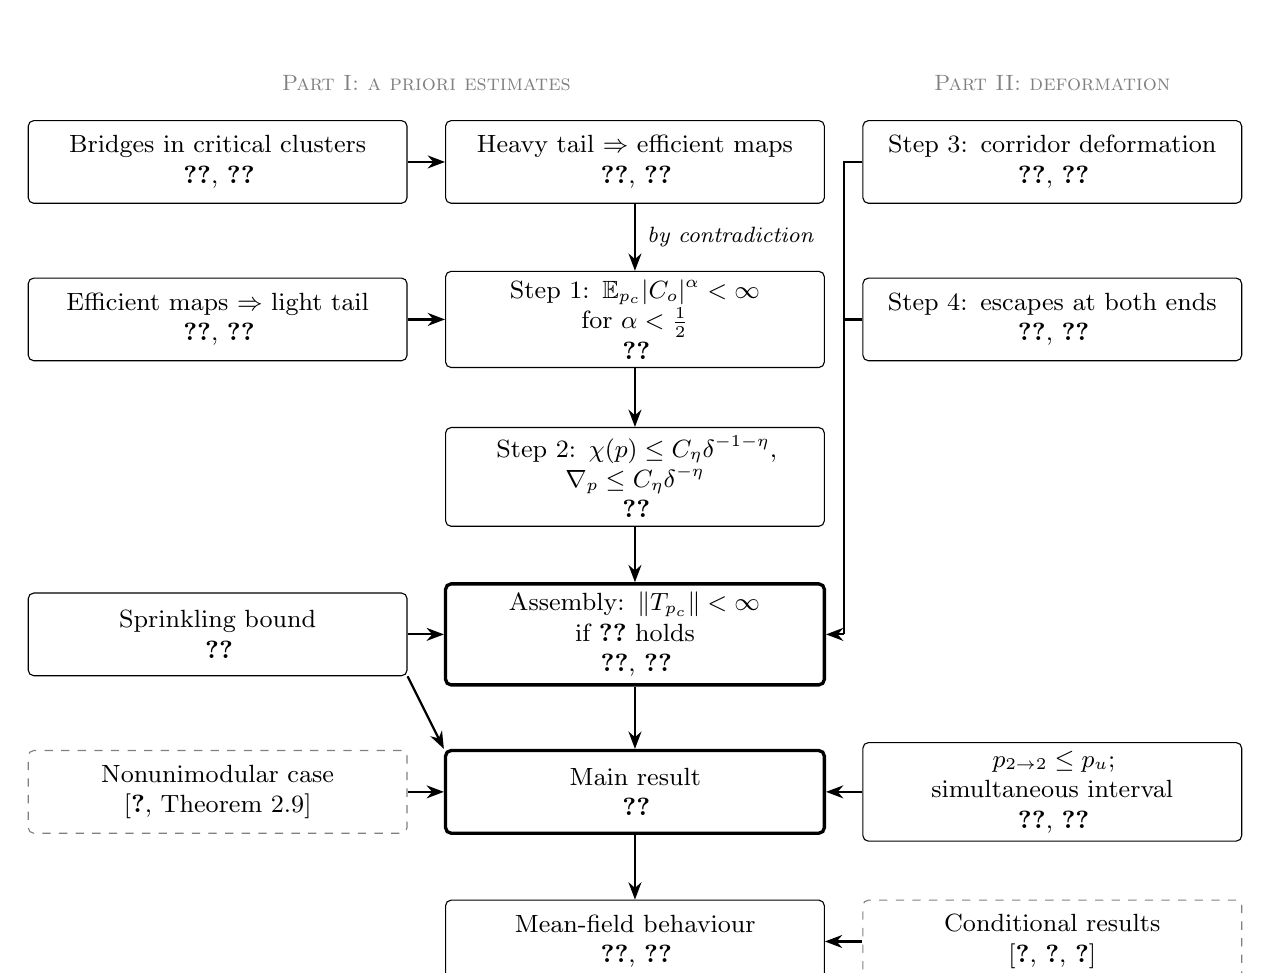
\begin{tikzpicture}[
    box/.style={draw, rounded corners=2pt, align=center, font=\small, text width=4.6cm,
                inner sep=3pt, minimum height=1.05cm,
                execute at begin node={\hyphenpenalty=10000\exhyphenpenalty=10000}},
    main/.style={box, very thick},
    cite/.style={box, draw=figgrey, dashed},
    arr/.style={-{Stealth[length=2.2mm]}, thick},
    lab/.style={font=\footnotesize\itshape, fill=white, inner sep=1pt}]
  % column headers
  \node[font=\footnotesize\scshape, text=figgrey] at (5.1,1.0) {Part I: a priori estimates};
  \node[font=\footnotesize\scshape, text=figgrey] at (13.05,1.0) {Part II: deformation};
  % Part I
  \node[box] (bridges) at (2.45,0)    {Bridges in critical clusters\\ \cref{prop:good}, \cref{sec:bridges}};
  \node[box] (ampl)    at (7.75,0)    {Heavy tail $\Rightarrow$ efficient maps\\ \cref{prop:amplification}, \cref{sec:maps}};
  \node[box] (eff)     at (2.45,-2.0) {Efficient maps $\Rightarrow$ light tail\\ \cref{prop:efficient}, \cref{sec:moments}};
  \node[box] (mom)     at (7.75,-2.0) {Step~1: \mbox{$\EE_{p_c}\abs{C_o}^\alpha<\infty$} for \mbox{$\alpha<\tfrac12$}\\ \cref{thm:moments}};
  \node[box] (apr)     at (7.75,-4.0) {Step~2: \mbox{$\chi(p)\le C_\eta\delta^{-1-\eta}$}, \mbox{$\nabla_p\le C_\eta\delta^{-\eta}$}\\ \cref{thm:apriori}};
  % Part II
  \node[box] (def)     at (13.05,0)    {Step~3: corridor deformation\\ \cref{prop:deformation}, \cref{sec:deformation}};
  \node[box] (esc)     at (13.05,-2.0) {Step~4: escapes at both ends\\ \cref{prop:escapes}, \cref{sec:escapes}};
  % assembly, the sprinkling bound and the main results
  \node[box]  (spr)    at (2.45,-6.0)  {Sprinkling bound\\ \cref{lem:sprinkling}};
  \node[main] (cb)     at (7.75,-6.0)  {Assembly: \mbox{$\norm{T_{p_c}}<\infty$} if \cref{ass:U} holds\\ \cref{thm:crit-bdd}, \cref{sec:assembly}};
  \node[cite] (nonu)   at (2.45,-8.0)  {Nonunimodular case\\ \cite[Theorem~2.9]{Hut19}};
  \node[box]  (aux)    at (13.05,-8.0) {\mbox{$\ptwo\le p_u$}; simultaneous interval\\ \cref{lem:p22-pu}, \cref{prop:interval}};
  \node[main] (thm)    at (7.75,-8.0)  {Main result\\ \cref{thm:main}};
  \node[cite] (hut)    at (13.05,-9.9) {Conditional results\\ \cite{DCT16,Hut20L2,Hut22sup}};
  \node[box]  (cons)   at (7.75,-9.9)  {Mean-field behaviour\\ \cref{thm:consequences}, \cref{sec:consequences}};
  % arrows inside Part I
  \draw[arr] (bridges) -- (ampl);
  \draw[arr] (ampl) -- node[lab, right=3pt] {by contradiction} (mom);
  \draw[arr] (eff) -- (mom);
  \draw[arr] (mom) -- (apr);
  \draw[arr] (apr) -- (cb);
  % Part II feeds the assembly through one bus
  \draw[thick] (def.west) -| (10.4,-6.0);
  \draw[thick] (esc.west) -- (10.4,-2.0);
  \draw[arr] (10.4,-6.0) -- (cb.east);
  % the sprinkling bound enters the assembly and the reduction
  \draw[arr] (spr) -- (cb);
  \draw[arr] (spr.south east) -- (thm.north west);
  % from critical boundedness to the main results
  \draw[arr] (cb) -- (thm);
  \draw[arr] (nonu) -- (thm);
  \draw[arr] (aux) -- (thm);
  \draw[arr] (thm) -- (cons);
  \draw[arr] (hut) -- (cons);
\end{tikzpicture}

\caption{Logical structure of the proof. An arrow points from a statement to a statement whose proof
uses it. Dashed boxes are results from the literature. Step~1 is proved by contradiction: if the
critical cluster size had an infinite moment of order $\alpha<1/2$, the amplification would produce
efficient endpoint maps, which force all such moments to be finite. The assembly
(\cref{sec:assembly}) combines the four steps with the sprinkling bound.}\label{fig:dependencies}
\end{figure}

\subsection{Reduction to critical boundedness}\label{sec:reduction}

The core of the argument is the following theorem.

\begin{theorem}[Critical boundedness]\label{thm:crit-bdd}
Assume \cref{ass:G,ass:U}. Then $\norm{T_{p_c}}<\infty$.
\end{theorem}

Everything else in \cref{thm:main} follows from \cref{thm:crit-bdd} and the tools of
\cref{sec:prelim}.

\begin{proof}[Proof of \cref{thm:main} given \cref{thm:crit-bdd}]
We first show that $T_{p_c}$ is bounded and $p_c<\ptwo$. If $\Aut(G)$ is unimodular,
$\norm{T_{p_c}}<\infty$ by \cref{thm:crit-bdd}. Since $p_c<1$ (\cref{lem:pc}), the sprinkling bound
(\cref{lem:sprinkling}) with a small $a>0$ then shows that $T_p$ is bounded at
$p=p_c+(1-p_c)a>p_c$, so $p_c<\ptwo$. If $\Aut(G)$ is not unimodular, then $p_c<\ptwo$ by a theorem of
Hutchcroft (\cref{prop:nonunimodular}). Since $T_p\le T_{p'}$ entrywise for $p\le p'$, the kernel
$T_p$ is bounded for every $p<\ptwo$ (\cref{lem:kernels}), in particular for $p=p_c$.

\Cref{lem:p22-pu} gives $\ptwo\le p_u$, and \cref{lem:kernels} identifies $\norm{T_{p_c}}$ with
$\sup_{p<p_c}\norm{T_p}$. This proves~\eqref{eq:main}. Finally, choose $p_c<p_1<p_2<\ptwo$. Then $T_{p_2}$
is bounded, and \cref{prop:interval} yields the simultaneous statement on $[p_1,p_2]$.
\end{proof}

\subsection{The mechanism: row sums versus norm}\label{sec:mechanism}

\paragraph{Row sums and norm.}
The connection kernel $T_p$ is nonnegative, symmetric and invariant, and its row sums equal $\chi(p)$.
By the Schur test (\cref{lem:kernels}), $\norm{T_p}\le\chi(p)$. Below $p_c$ the susceptibility is finite
by sharpness of the phase transition, so $T_p$ is bounded. The row sums, however, explode as
$p\uparrow p_c$: if $\chi$ stayed bounded, then $\chi(p_c)<\infty$ by monotone convergence, and the
sprinkling bound (\cref{lem:sprinkling}) would give $\chi(p)<\infty$ for some $p>p_c$, which is
impossible because $\theta(p)>0$. \Cref{thm:crit-bdd} therefore asserts that the norm of $T_p$ stays
bounded although its row sums do not. On a nonamenable graph this is possible because the $\ell^2$ norm
can be much smaller than the row sums. The basic example is the \emph{lazy simple random walk}
\begin{equation*}
  P(x,y)\coloneqq\frac{1}{2d}\,\1\{x\sim y\}+\frac12\,\1\{x=y\}\,,
  \qquad
  \rho\coloneqq\norm{P}<1\,,
\end{equation*}
whose row sums are one, while its norm is strictly smaller than one by nonamenability
(\cref{lem:walk}). We use $P$ and $\rho$ throughout.

\paragraph{What unboundedness would mean.}
Suppose that $\norm{T_{p_c}}=\infty$, and write $\delta\coloneqq p_c-p$ for $p<p_c$. Adding an
independent configuration of parameter $a$ to one of parameter $p$ and splitting open paths at the added
edges gives the sprinkling bound (\cref{lem:sprinkling})
\begin{align*}
  T_{p+(1-p)a}&\le\sum_{j\ge0}a^j\,T_p(\Adj\,T_p)^j\qquad\text{entrywise, and hence}\\
  \norm{T_{p+(1-p)a}}&\le\frac{\norm{T_p}}{1-ad\norm{T_p}}\qquad\text{if }ad\norm{T_p}<1\,.
\end{align*}
With $a=\delta/(1-p)$, so that $p+(1-p)a=p_c$, this turns a small norm at~$p$ into boundedness
at~$p_c$. Hence
\begin{equation}\label{eq:norm-lower}
  \norm{T_p}\ge\frac{1-p}{d\,\delta}\qquad\text{for all }p<p_c\,.
\end{equation}
Step~2 below shows that $\chi(p)\le C_\eta\delta^{-1-\eta}$ for every $\eta>0$. Hence the ratio
\begin{equation}\label{eq:R}
  R=R(p)\coloneqq\frac{\chi(p)}{\norm{T_p}}\in[1,\infty)
\end{equation}
satisfies $R\le C_\eta\delta^{-\eta}$ for every $\eta>0$: the norm of $T_p$ would agree with its row
sums up to a factor that is smaller than every power of $1/\delta$. We show that this is impossible by
deforming $T_p$ in a way that decreases its row sums by a large factor while decreasing its norm by at
most a factor two. This contradicts $\norm{\,\cdot\,}\le$ row sum.

\paragraph{Three structural facts.}
The comparison of norm and row sums rests on three properties of unimodular transitive graphs and of the
connection kernel, which we use throughout. First, the \emph{mass-transport principle}
(\cref{lem:mtp}): $\sum_yF(o,y)=\sum_xF(x,o)$ for every nonnegative function $F$ on $V\times V$ that is
invariant under the diagonal action of $\Aut(G)$; in particular every invariant kernel has equal row and
column sums. Second, for $p<p_c$ the kernel $T_p$ is \emph{positive semidefinite}
(\cref{lem:subcritical}). Third, the diagonal entry $\tr S\coloneqq S(o,o)$ of a bounded invariant
operator is a \emph{trace}: it is cyclic, and $\abs{\tr(BA)}\le\norm B\tr A$ for $A$ positive
semidefinite and $B$ self-adjoint (\cref{lem:trace}). Two consequences show how the decay of the
random walk on $\ell^2(V)$ enters. By the Cauchy--Schwarz inequality for $T_p$ and the trace,
\begin{equation*}
  (P^mT_p)(a,b)^2\le(P^mT_pP^m)(a,a)\,T_p(b,b)=\tr(P^{2m}T_p)\le\rho^{2m}\,:
\end{equation*}
a random walk of $m$ steps smooths the connection kernel at rate $\rho^m$, however large $\norm{T_p}$ is
(\cref{lem:smoothing}). And sums of the form $\sum_vP^k(o,v)\,T_p^3(v,o)=\tr(P^kT_p^3)$ are at most
$\rho^k\tr(T_p^3)=\rho^k\nabla_p$; this is how the triangle diagram enters the proof.

\paragraph{A deformation that separates the two.}
Fix an integer $k\ge3$ and let $w$ be a path of $k$ steps of the lazy walk, with probability $\mu(w)$
under~$P$. Erasing its loops produces a self-avoiding path $\gamma_w$ from $u=w_0$ to $v=w_k$. On the
\emph{corridor event} $\Cor_w$ all edges of $\gamma_w$ are open and all other edges at the interior
vertices of $\gamma_w$ are closed. Then $\gamma_w$ is an isolated open path, a \emph{corridor}. It joins
the clusters of $u$ and $v$ outside its interior, and it is their only open link unless these two
clusters coincide (\cref{fig:corridor}).
The deformation multiplies the indicator of $\{x\conn y\}$ by $\exp(-t\,c(w))$ for every corridor $w$
all of whose edges are pivotal for $x\conn y$, where $t\ge0$ is the deformation time and the weight
$c(w)=\mu(w)/\PP_p(\Cor_w)$ is calibrated so that each corridor is penalised at rate equal to its
random-walk probability. A penalised connection consists of a connection from $x$ to~$u$, a corridor,
and a connection from $v$ to~$y$. Summed over corridors, the rate at which the deformed kernel $T_t$
decreases is therefore at most $2\,T_pP^kT_p$, whose norm is at most $2\rho^k\norm{T_p}^2$. The rate
at which its row sum decreases is, roughly, the $\mu$-average of the product of the cluster masses at
$u$ and~$v$. Here no factor comparable to $\rho^k$ appears, since the row sums of $P^k$ equal one. Thus
over a time interval of length $(kR)^{C}/\norm{T_p}$ the norm changes by a negligible amount, while
the row sum, if the masses at the ends of corridors are comparable to the full row sum, decreases at a
rate proportional to its own square and must drop far below $\norm{T_p}$.

\paragraph{The three costs.}
Turning the last sentence into a proof requires three corrections, and each has a price.
\begin{enumerate}[label=(\roman*)]
  \item \emph{Distinct clusters.} The edges of a corridor are pivotal for $x\conn y$ only if the
  clusters of $u$ and $v$ outside the corridor are distinct. By the van den Berg--Kesten inequality
  and the trace bound above, the resulting error is at most
  $C\chi(p)^2\rho^k\nabla_p=CR^2\nabla_p\rho^k\norm{T_p}^2$
  (\cref{prop:deformation}\ref{it:def-rate}). It is negligible once $k$ is a large multiple of
  $\log R+\log\nabla_p$.
  \item \emph{Removing the corridor.} The cluster masses at $u$ and $v$ are computed after deleting the
  interior of the corridor, which may cut off most of the mass. Step~4 shows that for a positive
  fraction of paths $w$, both endpoints are joined by short paths avoiding the corridor to vertices
  whose connections to the neighbourhood of the corridor are tiny. Its key input is the smoothing bound
  above. Transporting the mass along these short paths costs a factor of order $(kR)^{-C}$.
  \item \emph{Interaction of corridors.} Penalties of different corridors on the same connection
  interact, which costs a factor $\e^{-tc_k}$ with $c_k=\e^{C_0k}$. This is harmless as long as
  $tc_k\ll1$ up to the final time $t\approx(kR)^C/\norm{T_p}$. By~\eqref{eq:norm-lower} this holds if
  $\e^{C_0k}(kR)^C\ll1/\delta$, in particular if $k$ and $\log R$ are $o(\log(1/\delta))$.
\end{enumerate}
The requirements (i) and (iii) can be met simultaneously if $\log R$ and $\log\nabla_p$ are
$o(\log(1/\delta))$: then $k$ can be chosen as a large multiple of
$\log R+\log\nabla_p+\log\log(1/\delta)$, which is still $o(\log(1/\delta))$. A bound
$R+\nabla_p\le C\delta^{-a}$ with a fixed $a>0$ would also do, but only if $a$ is smaller than a
threshold determined by constants of the construction (such as $C_0$ and the constants of Step~4) that
we do not control explicitly. This is why Step~2 proves the a priori bounds with an arbitrarily small
power of $1/\delta$.

\paragraph{Where the a priori bounds come from.}
Mean-field theory predicts $\PP_{p_c}(\abs{C_o}\ge n)\asymp n^{-1/2}$; \cref{thm:consequences} confirms
this a posteriori. Step~1 proves the weaker statement that $\EE_{p_c}\abs{C_o}^\alpha<\infty$ for every
$\alpha<1/2$. Step~2 converts it into the near-critical bounds. A decision-tree inequality transfers
the critical tail to $\chi(p)\le\delta^{-1-o(1)}$. A differential inequality for the triangle diagram
gives $\nabla_p\le\delta^{-o(1)}$; in it, the critical tail bounds the probability that two adjacent
distinct clusters are both large, and a concentration estimate bounds the number of edges between
them.

\paragraph{Critical moments by contradiction.}
Step~1 is proved by contradiction. If $\EE_{p_c}\abs{C_o}^\alpha=\infty$ for some $\alpha<1/2$, then at
infinitely many scales $n$ the probability that $\abs{C_o}\in[n,2n)$ is at least $n^{-\beta}$ for some
$\beta<1/2$: there are more large critical clusters than mean-field theory allows. We exploit them by
splicing independent small critical clusters onto a large one. This produces \emph{local endpoint
maps}, random rules that select a vertex of the cluster of the root, whose selection kernel has a very
small norm on $\ell^2(V)$ compared with their cost, measured by the logarithms of the inverse success
probability and of the cluster size. The multiplicity of the splicing is controlled by a bound on the
number of bridges in pieces cut out of critical clusters. Running such an efficient map slightly below
$p_c$ shows that $\chi$ grows at least as fast as a solution of $\chi'=\chi^{2-\gamma}$ for every
$\gamma>0$. This gives $\chi(p)\le\delta^{-1-o(1)}$ and hence a near-mean-field tail bound for the
critical cluster size, which contradicts the assumption. The susceptibility bound obtained in this way
is conditional on the heavy tail, which is used to construct the maps; Step~2 proves it unconditionally
from Step~1.

\subsection{Part I: a priori estimates (Steps 1 and 2)}\label{sec:part1}

\begin{theorem}[Step~1: critical moments]\label{thm:moments}
Assume \cref{ass:G,ass:U}. Then $\EE_{p_c}\abs{C_o}^\alpha<\infty$ for every $\alpha\in(0,1/2)$.
\end{theorem}

The proof of \cref{thm:moments} combines three propositions. The first concerns the geometry of
critical clusters. A \emph{bridge} of a finite connected graph~$H$ is an edge whose removal
disconnects~$H$. For vertices $x,y$ of~$H$ let $\dbr^H(x,y)$ be the number of bridges of~$H$ that
separate $x$ from~$y$; this is a pseudometric, the \emph{bridge distance}, and
$\diambr(H)\coloneqq\max_{x,y}\dbr^H(x,y)$ is the \emph{bridge diameter}. Throughout, a vertex set $B$
of an open cluster is regarded as a graph with the open edges joining its vertices.

\begin{definition}[Good clusters]\label{def:good}
Let $\varepsilon\in(0,1/2)$ and $\sigma\coloneqq1/2+\varepsilon$. A finite open cluster~$C$ with
$\abs{C}\le M$ is \emph{$M$-good} if the following holds for every $A\subseteq C$ and every connected
component $B$ of the open subgraph induced by $C\setminus A$: if the set $\mathcal K$ of open edges
between $B$ and $A$ is not empty, then $\diambr(B)\le\abs{\mathcal K}M^\sigma$.
\end{definition}

\begin{proposition}[Step~1a: bridges in critical clusters]\label{prop:good}
Assume \cref{ass:G} and let $\varepsilon\in(0,1/2)$. For all sufficiently large~$M$,
\begin{equation*}
  \PP_{p_c}\bigl(\abs{C_o}\le M \text{ and } C_o \text{ is not $M$-good}\bigr)\le\exp(-M^\varepsilon)\,.
\end{equation*}
Moreover, the event $\{\abs{C_o}\le M,\ C_o\text{ is $M$-good}\}$ is determined by the states of the
edges with an endpoint in $B(o,M)$.
\end{proposition}

In a critical branching process of total size~$M$, every edge is a bridge and the height is of order
$M^{1/2}$; heuristically, critical clusters on a nonamenable graph behave alike. \Cref{prop:good} is a
robust form of this heuristic: pieces cut out of a critical cluster have bridge diameter at most
$M^{1/2+\varepsilon}$ per cut edge, outside an event of stretched-exponentially small probability. It
is proved in \cref{sec:bridges} by an exploration-martingale bound on the number of pivotal edges of a
marked cluster. The exponent $\sigma$ enters the next step through the requirement $\beta+\sigma<1$.

\begin{definition}[Local endpoint maps]\label{def:map}
A \emph{local endpoint map} is a family $\Phi=(\Phi_x)_{x\in V}$ of functions
$\Phi_x\colon\{0,1\}^E\times V\to[0,1]$ with $\sum_y\Phi_x(\omega,y)\le1$, to be read as a randomised
rule: given the configuration~$\omega$, the rule at $x$ outputs $y$ with probability
$\Phi_x(\omega,y)$ and fails with the remaining probability. We require that there is $r_\Phi<\infty$
such that $\Phi_x(\omega,\cdot)$ depends only on the states of the edges with an endpoint in
$B(x,r_\Phi)$, that $\Phi_x(\omega,y)=0$ unless $y\in C_x(\omega)$, and that
$\Phi_{gx}(g\omega,gy)=\Phi_x(\omega,y)$ for all $g\in\Aut(G)$. The map has \emph{cap}~$M\in\N$ if
$\Phi_x(\omega,\cdot)\equiv0$ unless $\abs{C_x}\le M$ and $C_x$ is $M$-good. Its \emph{success
probability}, \emph{endpoint kernel} and \emph{kernel norm} are
\begin{equation*}
  s\coloneqq\EE_{p_c}\sum_{y}\Phi_x(\omega,y)\,,\qquad
  K(x,y)\coloneqq\frac{\EE_{p_c}\Phi_x(\omega,y)}{s}\,,\qquad
  r\coloneqq\norm{K}\,;
\end{equation*}
by invariance $s$ does not depend on~$x$. If $s>0$ and $r<1$, the \emph{efficiency ratio} of~$\Phi$ is
\begin{equation*}
  \operatorname{eff}(\Phi)\coloneqq\frac{\log(1/s)+\log M}{\log(1/r)}\,.
\end{equation*}
\end{definition}

Thus $K(x,y)$ is the probability that the rule at $x$ outputs~$y$, given that it succeeds; caps refer
to $M$-goodness for the parameter $\varepsilon$ of \cref{def:good}, which is kept fixed. Under
\cref{ass:U} the endpoint kernel is doubly stochastic, so $r\le1$ (\cref{lem:map-basic}). A small
efficiency ratio means that the selected vertex is spread out very widely, as measured on $\ell^2(V)$,
at a moderate price in success probability and cluster size. Steps of the lazy random walk along open
edges give a first map with $r<\e^{-1}$ (\cref{lem:start}); the point of the next proposition is to make
the efficiency ratio small.

\begin{proposition}[Step~1b: heavy tails yield efficient maps]\label{prop:amplification}
Assume \cref{ass:G,ass:U}, and suppose that $\EE_{p_c}\abs{C_o}^{\alpha}=\infty$ for some
$\alpha\in(0,1/2-\varepsilon)$. Then there are local endpoint maps with cap $M\ge2$ and $r<\e^{-1}$
whose efficiency ratios are arbitrarily small.
\end{proposition}

The proof in \cref{sec:maps} improves a given map~$\Phi$ in one \emph{amplification step}, at a heavy
scale~$n$, that is, a scale with $\PP_{p_c}(n\le\abs{C_o}<2n)\ge n^{-\beta}$ for some fixed
$\beta<1/2-\varepsilon$. For a root $x$, let $A$ be the cluster of $x$ in a first configuration, and
for a vertex $z$ run $\ell$ steps of $\Phi$ from~$z$, each in a fresh independent configuration. If
$n\le\abs A<2n$ and the last step lands in~$A$, we splice the pieces of the $\ell$ old clusters onto~$A$
by exchanging finitely many edge states between the configurations. Afterwards $z$ lies in the cluster
of~$x$, which has fewer than $2n+\ell M$ vertices. The new map at $x$ outputs $z$ with probability
proportional to the total weight of the splicings that produce the observed configuration and end
at~$z$. Its endpoint kernel is essentially the $\ell$-th power of the old one composed with a stochastic
kernel, so $\log(1/r)$ is multiplied by about~$\ell$. Since the old kernel is doubly stochastic, summing
over $z$ the probability that the chain from $z$ succeeds and ends in $A$ gives $s^\ell\abs A$; this
makes the new success probability of order $\PP_{p_c}(n\le\abs{C_o}<2n)\ge n^{-\beta}$, up to a factor
polynomial in $\ell$ and~$M$. The cap is about $2n$. To control fluctuations, the splicing must be
undone: once the positions of the $\ell$ seams among the bridges of the final cluster are known,
everything else is determined, and \cref{prop:good} bounds the number of possible seam positions,
weighted by the probabilities of choosing them, by about $M^{\sigma\ell}$. A second-moment estimate
needs this number to be at most $ns^\ell$, which is why the number of steps can be as large as about
$\log n/(\log(1/s)+\sigma\log M)$. With this choice, each amplification step multiplies the ratio
$(\log(1/s)+\sigma\log M)/\log(1/r)$ by a factor close to $\beta+\sigma<1$.

\begin{proposition}[Step~1c: efficient maps yield light tails]\label{prop:efficient}
Assume \cref{ass:G,ass:U}, and suppose that there are local endpoint maps with cap $M\ge2$ and
$r<\e^{-1}$ whose efficiency ratios are arbitrarily small. Then
$\EE_{p_c}\abs{C_o}^\alpha<\infty$ for every $\alpha\in(0,1/2)$.
\end{proposition}

The proof in \cref{sec:moments} runs a fixed efficient map at parameter $p$ slightly below $p_c$; its
cap is used only through $\abs{C_x}\le M$, not through goodness. Starting from the root of an
independent, size-biased cluster~$A$, iterates of the endpoint kernel spread so quickly that after
$\ell\approx\log\chi(p)/\log(1/r)$ steps the endpoint has left $A$, and the susceptibility in
$V\setminus A$ at the endpoint is comparable to $\chi(p)$. On the other hand, a successful output lies
within $M$ open steps of its input, and moving along at most $M$ open edges increases the
susceptibility in $V\setminus A$ by a factor at most of order $M$ (\cref{lem:intrinsic-ball}); after
dividing by the success probability, one step of the map multiplies it by at most a factor $Z\le CM/s$,
up to a contribution from the boundary of~$A$. The boundary contribution is controlled by the quantity
\begin{equation*}
  \Delta(p)\coloneqq\chi(p)^{-2}\sum_{b\sim o}\EE_p\bigl[\abs{C_o}\,\abs{C_b};\,C_o\neq C_b\bigr]
  =(1-p)\,\frac{\chi'(p)}{\chi(p)^2}\,,
\end{equation*}
where the identity holds for almost every $p$ by Russo's formula. Comparing the two bounds gives
$\Delta(p)\ge cZ^{-\ell}$, that is, $\chi'\ge c\chi^{2-\gamma}$ with $\gamma\approx\operatorname{eff}(\Phi)$,
and so $\chi(p)\le C\delta^{-1/(1-\gamma)}$. A comparison of explorations at $p$ and at $p_c$ then bounds
the critical tail: $\PP_{p_c}(\abs{C_o}\ge N)\le N^{-1/2+o(1)}$.

\begin{proof}[Proof of \cref{thm:moments} given \cref{prop:amplification,prop:efficient}]
Suppose that $\EE_{p_c}\abs{C_o}^{\alpha_0}=\infty$ for some $\alpha_0\in(0,1/2)$, and choose the
parameter of \cref{def:good} as some $\varepsilon\in(0,1/2-\alpha_0)$. By \cref{prop:amplification}, the
hypothesis of \cref{prop:efficient} holds, and \cref{prop:efficient} gives
$\EE_{p_c}\abs{C_o}^{\alpha_0}<\infty$, a contradiction.
\end{proof}

\begin{theorem}[Step~2: near-critical a priori bounds]\label{thm:apriori}
Assume \cref{ass:G,ass:U}. For every $\eta>0$ there is $C_\eta<\infty$ such that
\begin{align}
  \chi(p)&\le C_\eta\,(p_c-p)^{-1-\eta}&&\text{for all }p\in[0,p_c)\,,\label{eq:apriori-chi}\\
  \nabla_p&\le C_\eta\,(p_c-p)^{-\eta}&&\text{for all }p\in[p_c/2,p_c)\,.\label{eq:apriori-triangle}
\end{align}
\end{theorem}

Both bounds are proved from \cref{thm:moments}. The susceptibility bound~\eqref{eq:apriori-chi}
(\cref{sec:chi}) follows from a differential inequality for $\PP_p(\abs{C_o}\ge n)$ in~$p$, obtained from
the decision-tree inequality of O'Donnell, Saks, Schramm and Servedio, applied to an algorithm that
marks every vertex independently with probability $1/n$ and explores the clusters of the marked
vertices. The triangle bound~\eqref{eq:apriori-triangle} (\cref{sec:triangle}) follows from a
differential inequality for $\nabla_p$. By Russo's formula, $\nabla_p'$ is a sum over pairs of distinct
clusters, weighted by the number of edges between them and by a kernel built from $T_p$. Pairs with a
small cluster contribute at most a power of the size cutoff times $\nabla_p$. For two large clusters,
Step~1 bounds the probability that two adjacent distinct clusters are both large, and the number of
edges between them is controlled by comparing two explorations of one cluster, with and without the
other cluster removed. The centred scores of the two explorations differ by exactly $-p$ times this
number, and each score is concentrated.

\subsection{Part II: the corridor deformation (Steps 3 and 4)}\label{sec:part2}

We now define the deformation precisely. Throughout this subsection $p\in[p_c/2,p_c)$ and $k\ge3$ are
fixed, and $q\coloneqq1-p$.

\begin{definition}[Corridors and the deformed kernel]\label{def:deformation}
A \emph{raw path} is a sequence $w=(w_0,\dots,w_k)$ of vertices with $P(w_{i-1},w_i)>0$ for all~$i$;
it has \emph{base} $w_0$, \emph{end} $w_k$ and probability $\mu(w)\coloneqq\prod_{i=1}^kP(w_{i-1},w_i)$.
Delete the holding steps $w_{i-1}=w_i$ and erase the loops of the remaining path in chronological
order. This gives a self-avoiding path $\gamma_w$ from $w_0$ to $w_k$ with $\abs{\gamma_w}$ edges. Its
\emph{interior} $I_w$ is the set of its vertices other than $w_0$ and $w_k$, and $\Lambda_w\coloneqq
V\setminus I_w$. The \emph{blockers} $\Bl_w$ are the edges incident to $I_w$ that are not edges
of~$\gamma_w$. The raw path is a \emph{template} if $\abs{\gamma_w}\ge3$. Its \emph{corridor event}
$\Cor_w$ is the event that all edges of $\gamma_w$ are open and all blockers are closed, and its
\emph{weight} is
\begin{equation*}
  c(w)\coloneqq\mu(w)\,p^{-\abs{\gamma_w}}\,q^{-\abs{\Bl_w}}\,,\qquad\text{so that}\qquad
  c(w)\,\PP_p(\Cor_w)=\mu(w)\,.
\end{equation*}
For a domain $\Lambda\subseteq V$ and $x,y\in\Lambda$, a template
$w$ is \emph{counted} for $(x,y)$ in~$\Lambda$ if all vertices of $\gamma_w$ lie in~$\Lambda$, every
edge of $\gamma_w$ is open and \emph{pivotal} for $x\connin{\Lambda}y$ (that is, $x\connin{\Lambda}y$
holds and fails after closing this edge), and every blocker is closed or has an endpoint outside
$\Lambda$. With the sum over all templates~$w$ of any base, define
\begin{equation*}
  N^\Lambda_{xy}\coloneqq\sum_{w\text{ counted for }(x,y)\text{ in }\Lambda}c(w)\,,\qquad
  W^\Lambda_t(x,y)\coloneqq\1\{x\connin{\Lambda}y\}\,\e^{-tN^\Lambda_{xy}}\qquad(t\ge0)\,,
\end{equation*}
and $W^\Lambda_t(x,y)\coloneqq0$ if $x\notin\Lambda$ or $y\notin\Lambda$. The \emph{deformed
susceptibilities} and the \emph{deformed kernel} are
\begin{equation*}
  \chi^\Lambda_t(x)\coloneqq\EE_p\sum_{y\in V}W^\Lambda_t(x,y)\,,\qquad
  \chi_t\coloneqq\chi^V_t(o)\,,\qquad
  T_t(x,y)\coloneqq\EE_p\,W^V_t(x,y)\,.
\end{equation*}
Finally, $\Erw[F(w)]\coloneqq\sum_w\mu(w)F(w)$ denotes the average over $k$-step lazy-walk paths $w$ with
base $w_0=o$.
\end{definition}

At $t=0$ nothing is penalised: $T_0=T_p$ and $\chi_0=\chi(p)$. Different raw paths with the same
loop erasure are different templates, and the convention for blockers outside~$\Lambda$ lets us compare
domains without changing the weights.

\begin{figure}[ht]
\centering
% A corridor on the event Cor_w (schematic)
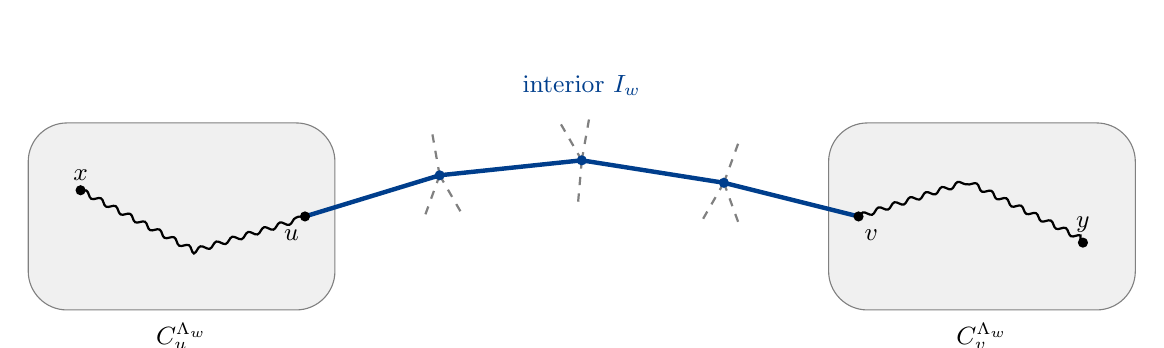
\begin{tikzpicture}[scale=0.95,
    vtx/.style={circle, fill, inner sep=1.3pt},
    blob/.style={draw=figgrey, fill=figgrey!12, rounded corners=14pt},
    corr/.style={figmain, line width=1.6pt},
    blk/.style={figgrey, dashed, thick},
    leg/.style={black, thick, decorate, decoration={snake, amplitude=0.9pt, segment length=6pt}}]
  % exterior clusters
  \draw[blob] (-2.6,-1.25) rectangle (1.5,1.25);
  \draw[blob] (8.1,-1.25) rectangle (12.2,1.25);
  \node[font=\small] at (-0.55,-1.6) {$C_u^{\Lambda_w}$};
  \node[font=\small] at (10.15,-1.6) {$C_v^{\Lambda_w}$};
  % corridor
  \coordinate (u) at (1.1,0);
  \coordinate (a) at (2.9,0.55);
  \coordinate (b) at (4.8,0.75);
  \coordinate (c) at (6.7,0.45);
  \coordinate (v) at (8.5,0);
  \draw[corr] (u) -- (a) -- (b) -- (c) -- (v);
  % closed blockers at interior vertices
  \foreach \p/\ang in {a/100, a/250, a/300, b/80, b/120, b/265, c/70, c/240, c/290} {
    \draw[blk] (\p) -- ++(\ang:0.6);
  }
  \foreach \p in {a,b,c} \node[vtx, figmain] at (\p) {};
  \node[vtx] at (u) {};
  \node[vtx] at (v) {};
  \node[font=\small, anchor=north east] at (1.15,-0.05) {$u$};
  \node[font=\small, anchor=north west] at (8.45,-0.05) {$v$};
  \node[font=\small, text=figmain] at (4.8,1.75) {interior $I_w$};
  % terminals and exterior legs
  \coordinate (x) at (-1.9,0.35);
  \coordinate (y) at (11.5,-0.35);
  \draw[leg] (x) -- (-0.4,-0.45) -- (u);
  \draw[leg] (v) -- (9.9,0.45) -- (y);
  \node[vtx] at (x) {};
  \node[vtx] at (y) {};
  \node[font=\small, anchor=south] at (x) {$x$};
  \node[font=\small, anchor=south] at (y) {$y$};
\end{tikzpicture}

\caption{A corridor on the event $\Cor_w$ (schematic). The loop-erased path $\gamma_w$ (thick) is
open, and every other edge at its interior $I_w$ is closed (dashed). Its edges are all pivotal for
$x\conn y$ if and only if $x$ and $y$ lie in the clusters $C_u^{\Lambda_w}$ and $C_v^{\Lambda_w}$ of its
endpoints in $\Lambda_w=V\setminus I_w$, in either order, and these two clusters are distinct
(\cref{lem:calibration}).}\label{fig:corridor}
\end{figure}

\begin{proposition}[Step~3: properties of the deformation]\label{prop:deformation}
Assume \cref{ass:G,ass:U}. There is $C_0\ge1$, depending only on~$G$, such that, with
$c_k\coloneqq\e^{C_0k}$, the following holds for all $p\in[p_c/2,p_c)$, $k\ge3$ and $t\ge0$.
\begin{enumerate}[label=\textup{(\alph*)}]
  \item\label{it:def-basic} \emph{Basic bounds.} $T_t$ is symmetric and invariant,
  $0\le T_t\le T_p$ entrywise, and $\norm{T_t}\le\chi_t\le\chi(p)$. The function $t\mapsto\chi_t$ is
  continuously differentiable on $[0,\infty)$.
  \item\label{it:def-norm} \emph{The norm barely moves.}
  $\norm{T_t}\ge\norm{T_p}-2t\rho^k\norm{T_p}^2$.
  \item\label{it:def-rate} \emph{The row sum decreases.}
  \begin{equation*}
    -\frac{\d}{\d t}\chi_t\ge\e^{-tc_k}\Bigl(\Erw\bigl[\1\{\abs{\gamma_w}\ge3\}\,
    \chi^{\Lambda_w}_t(w_0)\,\chi^{\Lambda_w}_t(w_k)\bigr]-C_0\,\chi(p)^2\rho^k\,\nabla_p\Bigr)\,.
  \end{equation*}
  \item\label{it:def-deletion} \emph{Deletion.} For every domain $\Lambda$, every $A\subseteq V$ and
  every $z\in V$,
  $\chi^{\Lambda\setminus A}_t(z)\ge\chi^\Lambda_t(z)-\chi(p)\sum_{b\in\Nb[A]}T_p(z,b)$.
  \item\label{it:def-path} \emph{Transport along a path.} If $\Lambda$ contains a self-avoiding path
  of length~$l$ from $b$ to~$z$, then $\chi^\Lambda_t(b)\ge\e^{-tlc_k}p^l\chi^\Lambda_t(z)$.
\end{enumerate}
\end{proposition}

Items~\ref{it:def-norm} and~\ref{it:def-rate} are the two halves of the comparison described in
\cref{sec:mechanism}. Item~\ref{it:def-norm} holds because a penalised connection factors through a
corridor, so that $T_p-T_t\le2t\,T_pP^kT_p$ entrywise. Item~\ref{it:def-rate} is obtained by moving
the root of the susceptibility to the base of the corridor with the mass-transport principle: the
calibration $c(w)\PP_p(\Cor_w)=\mu(w)$ then produces the average over raw paths, and the two exterior
clusters contribute the product of the deformed susceptibilities at the two ends. The error term
accounts for the requirement that the exterior clusters be distinct and is bounded with the
van den Berg--Kesten inequality and the trace. The factor $\e^{-tc_k}$ is the price for the penalties
of corridors that overlap the given one. Items~\ref{it:def-deletion} and~\ref{it:def-path} are the
tools that make the main term of~\ref{it:def-rate} usable: deleting a set $A$ can only destroy the
connections that pass near~$A$, and an open path transports mass at the cost of its probability.
\Cref{prop:deformation} is proved in \cref{sec:deformation}.

\begin{proposition}[Step~4: escapes at both ends]\label{prop:escapes}
Assume \cref{ass:G,ass:U}. There are $J,k_0\in\N$ and $C_1,c_\star>0$, depending only on~$G$, with the
following property. Let $p\in[p_c/2,p_c)$, $k\ge k_0$ and $R\ge1$, and put
$j\coloneqq J+\lceil C_1\log((k+1)R)\rceil$. Let $\mathcal W$ be the set of raw paths $w$ with
$\abs{\gamma_w}\ge3$ such that each of $w_0$ and $w_k$ is joined by a self-avoiding path in
$\Lambda_w$ of length at most $j$ to a vertex~$z$ with
\begin{equation*}
  \sum_{b\in\Nb[I_w]}T_p(z,b)\le\frac{1}{4R}\,.
\end{equation*}
Then $\Erw[\1\{w\in\mathcal W\}]\ge c_\star$.
\end{proposition}

The vertices $z$ are \emph{escapes}: from them, deleting the corridor costs little in
\cref{prop:deformation}\ref{it:def-deletion}. The proof in \cref{sec:escapes} lets the raw path begin
and end with halves of geodesic segments, and lets the escapes leave along the opposite halves and then
continue as independent random walks of length $m$ of order $C_1\log((k+1)R)$. Avoidance of the raw
path follows from the decay of $P^l$ on $\ell^2(V)$. The construction is symmetric under reversal of the
raw path, and the mass-transport principle turns this symmetry into an identity of probabilities, which
transfers the avoidance estimate from one endpoint to the other. Finally, the walks smooth the
connection kernel, $(P^mT_p)(a,b)\le\rho^m$, which makes the sum over $\Nb[I_w]$ small.

\subsection{Proof of critical boundedness}\label{sec:assembly}

We now prove \cref{thm:crit-bdd} from the four steps and the sprinkling bound.

\begin{proof}[Proof of \cref{thm:crit-bdd}]
Suppose, for a contradiction, that $\norm{T_{p_c}}=\infty$. For $p\in[p_c/2,p_c)$ put
\begin{equation*}
  \delta\coloneqq p_c-p\,,\qquad S\coloneqq\log(1/\delta)\,,\qquad R\coloneqq\frac{\chi(p)}{\norm{T_p}}\ge1\,.
\end{equation*}
All limits below are taken as $\delta\downarrow0$, that is, $p\uparrow p_c$.

\emph{Stage 1: size of the parameters.}
By~\eqref{eq:norm-lower}, which follows from \cref{lem:sprinkling}, $\norm{T_p}\ge(1-p_c)/(d\delta)$,
so $\log\norm{T_p}\ge S-C$. By
\cref{thm:apriori}, for every $\eta>0$ we have $R\le C_\eta\delta^{-1-\eta}\cdot d\delta/(1-p_c)\le
C'_\eta\delta^{-\eta}$ and $\nabla_p\le C_\eta\delta^{-\eta}$. Hence
\begin{equation}\label{eq:assembly-subpower}
  \log R=o(S)\qquad\text{and}\qquad\log\nabla_p=o(S)\,.
\end{equation}

\emph{Stage 2: choice of the constants.}
Fix the constants $J,k_0,C_1,c_\star$ of \cref{prop:escapes}; they do not depend on~$p$. Since $p\ge p_c/2$ and $j\le J+1+C_1\log((k+1)R)$, we have
\begin{equation}\label{eq:assembly-pj}
  p^{2j}\ge c_2\,(kR)^{-C_2}\qquad\text{for all }k\ge1\text{ and }R\ge1\,,
\end{equation}
with $C_2\coloneqq2C_1\log(2/p_c)$ and $c_2\coloneqq(p_c/2)^{2J+2}\,2^{-C_2}$. Let
$\lambda\coloneqq\log(1/\rho)>0$, fix $K_\star>0$ with $\kappa_\star\coloneqq\lambda K_\star>C_2+4$, and set
\begin{equation*}
  A_\delta\coloneqq\log(2R)+\log(2+\nabla_p)+\log S\,,\qquad
  k\coloneqq\lceil K_\star A_\delta\rceil\,,\qquad
  D_\star\coloneqq(kR)^{C_2+2}\,,\qquad
  t_\star\coloneqq\frac{D_\star}{\norm{T_p}}\,.
\end{equation*}
By~\eqref{eq:assembly-subpower}, $k\to\infty$ and $k=o(S)$; in particular $k\ge\max\{k_0,3\}$ and
$k\le S$ for small~$\delta$. We claim that
\begin{equation}\label{eq:assembly-small}
  D_\star\rho^k\to0\,,\qquad(kR)^{C_2}R^2\nabla_p\,\rho^k\to0\,,\qquad t_\star jc_k\to0\,.
\end{equation}
Indeed, $\rho^k\le\e^{-\lambda K_\star A_\delta}=(2R)^{-\kappa_\star}(2+\nabla_p)^{-\kappa_\star}
S^{-\kappa_\star}$. Since $R,\nabla_p\ge1$ and $k\le S$, this gives
$D_\star\rho^k\le S^{C_2+2-\kappa_\star}\to0$ and
$(kR)^{C_2}R^2\nabla_p\,\rho^k\le S^{C_2-\kappa_\star}\to0$. Finally, $c_k=\e^{C_0k}$ and
$\log\norm{T_p}\ge S-C$ give
\begin{equation*}
  \log(t_\star jc_k)\le(C_2+2)(\log k+\log R)-S+C+\log j+C_0k=-S+o(S)\,,
\end{equation*}
by~\eqref{eq:assembly-subpower}, $k=o(S)$ and $j=O(\log(kR))$.

\emph{Stage 3: the norm stays large.}
Consider the deformation of \cref{def:deformation} with these $p$ and~$k$, for $t\in[0,t_\star]$. By
\cref{prop:deformation}\ref{it:def-norm} and~\eqref{eq:assembly-small}, for small $\delta$,
\begin{equation}\label{eq:assembly-norm}
  \norm{T_t}\ge\norm{T_p}\bigl(1-2t_\star\rho^k\norm{T_p}\bigr)=\norm{T_p}(1-2D_\star\rho^k)\ge\tfrac12\norm{T_p}\,,
  \qquad\text{hence}\qquad
  \chi_t\ge\tfrac12\norm{T_p}
\end{equation}
by \cref{prop:deformation}\ref{it:def-basic}.

\emph{Stage 4: the row sum decreases quadratically.}
Let $w\in\mathcal W$, the set of \cref{prop:escapes} for our $p$, $k$ and~$R$, and let $z$ be the
escape vertex of the endpoint $w_0$. The deformation is invariant, so $\chi_t^V(z)=\chi_t$. By
\cref{prop:deformation}\ref{it:def-deletion} with $\Lambda=V$ and $A=I_w$, then $\chi(p)=R\norm{T_p}$
and~\eqref{eq:assembly-norm},
\begin{equation*}
  \chi^{\Lambda_w}_t(z)\ge\chi_t-\frac{\chi(p)}{4R}=\chi_t-\tfrac14\norm{T_p}\ge\tfrac12\chi_t\,.
\end{equation*}
\Cref{prop:deformation}\ref{it:def-path}, applied along the escape path of length at most~$j$ in
$\Lambda_w$, gives $\chi^{\Lambda_w}_t(w_0)\ge\e^{-tjc_k}p^j\chi_t/2$, and the same bound holds at~$w_k$.
Since $\e^{-2t_\star jc_k}\ge1/2$ for small~$\delta$ by~\eqref{eq:assembly-small}, the bound
\eqref{eq:assembly-pj} and $\Erw[\1\{w\in\mathcal W\}]\ge c_\star$ yield, for all $t\in[0,t_\star]$,
\begin{equation*}
  \Erw\bigl[\1\{\abs{\gamma_w}\ge3\}\,\chi^{\Lambda_w}_t(w_0)\,\chi^{\Lambda_w}_t(w_k)\bigr]
  \ge c_\star\cdot\tfrac12\,p^{2j}\cdot\tfrac14\chi_t^2
  \ge\tfrac18c_\star c_2\,(kR)^{-C_2}\chi_t^2\,.
\end{equation*}
The error term in \cref{prop:deformation}\ref{it:def-rate} satisfies, by $\chi(p)=R\norm{T_p}\le2R\chi_t$
and~\eqref{eq:assembly-small},
\begin{equation*}
  C_0\,\chi(p)^2\rho^k\nabla_p\le4C_0\,R^2\nabla_p\,\rho^k\,\chi_t^2=o\bigl((kR)^{-C_2}\bigr)\,\chi_t^2\,.
\end{equation*}
Since also $\e^{-tc_k}\ge1/2$ for $t\le t_\star$, \cref{prop:deformation}\ref{it:def-rate} gives, for
small~$\delta$,
\begin{equation}\label{eq:assembly-ode}
  -\frac{\d}{\d t}\chi_t\ge c_3\,(kR)^{-C_2}\chi_t^2\qquad\text{for all }t\in[0,t_\star]\,,
  \qquad c_3\coloneqq c_\star c_2/32\,.
\end{equation}

\emph{Stage 5: contradiction.}
The function $t\mapsto\chi_t$ is positive and continuously differentiable, so~\eqref{eq:assembly-ode}
integrates to
\begin{equation*}
  \frac{1}{\chi_{t_\star}}\ge\frac1{\chi_0}+c_3\,(kR)^{-C_2}t_\star\ge c_3\,\frac{(kR)^2}{\norm{T_p}}\,.
\end{equation*}
By~\eqref{eq:assembly-norm}, $1/\chi_{t_\star}\le2/\norm{T_p}$. Hence $c_3(kR)^2\le2$, which fails for
small~$\delta$ because $k\to\infty$. This contradiction proves $\norm{T_{p_c}}<\infty$.
\end{proof}

\begin{remark}[Order of the choices]\label{rem:order}
The constants $J,k_0,C_1,c_\star$ of the escape construction and $C_0$ of the deformation depend only
on~$G$; they are fixed before $p$ is chosen. The length $k$ and the final time $t_\star$ are then chosen
as functions of $p$ through $R$, $\nabla_p$ and $S$. The a priori bounds of Step~2 are used only
through~\eqref{eq:assembly-subpower}.
\end{remark}

\subsection{Roadmap}\label{sec:roadmap}

\Cref{fig:dependencies} shows how the statements depend on each other. Part~I
(\cref{sec:bridges,sec:maps,sec:moments,sec:triangle}) establishes the a priori estimates. It only
concerns critical and near-critical percolation and does not involve the deformation. Part~II
(\cref{sec:deformation,sec:escapes}) holds at every fixed $p\in[p_c/2,p_c)$ and uses only subcritical
facts; the two parts meet only in the proof above.

\section{Preliminaries}\label{sec:prelim}

This section collects the tools used in the proof. Classical results are quoted; proofs are given for
the variants that are less standard.

\subsection{Kernels and operators}\label{sec:kernels}

For a kernel~$K$ we use the operator norm
\begin{equation*}
  \norm{K}\coloneqq\sup\Bigl\{\Bigl|\sum_{x,y}\overline{g(x)}K(x,y)f(y)\Bigr|\colon
  f,g\text{ finitely supported},\ \norm{f}_2=\norm{g}_2=1\Bigr\}\in[0,\infty]\,.
\end{equation*}
If it is finite, $K$ extends to a bounded operator on $\ell^2(V)$ whose matrix is~$K$; conversely, a
bounded operator $S$ has the matrix $S(x,y)=\langle\1_x,S\1_y\rangle$, where $\1_x$ is the indicator
function of~$\{x\}$. We identify the two.
For a nonnegative kernel $L$ and vertex sets $A,B$ we write
\begin{equation*}
  L(A,B)\coloneqq\sum_{a\in A}\sum_{b\in B}L(a,b)\,;
\end{equation*}
for instance, $\Adj(A,B)$ is the number of edges with one endpoint in $A$ and the other in~$B$.

\begin{lemma}[Kernel bounds]\label{lem:kernels}
Let $K$ and $L$ be kernels with $L\ge0$.
\begin{enumerate}[label=\textup{(\alph*)}]
  \item\label{it:domination} \emph{Domination.} If $\abs{K}\le L$ entrywise, then $\norm{K}\le\norm{L}$.
  \item\label{it:schur} \emph{Schur test.} If all row sums and all column sums of $L$ are at most~$b$,
  then $\norm{L}\le b$.
  \item\label{it:monotone} \emph{Monotone limits.} For $0<p_*\le1$ and all $x,y$,
  $T_p(x,y)\uparrow T_{p_*}(x,y)$ as $p\uparrow p_*$, and
  $\norm{T_{p_*}}=\sup_{p<p_*}\norm{T_p}\in[0,\infty]$. Moreover $T_p\le T_{p'}$ entrywise for
  $p\le p'$; in particular $T_p$ is bounded for every $p<\ptwo$.
\end{enumerate}
\end{lemma}

\begin{proof}
For~\ref{it:domination}, $\abs{\sum\overline{g(x)}K(x,y)f(y)}\le\sum\abs{g(x)}L(x,y)\abs{f(y)}
\le\norm{L}\norm{f}_2\norm{g}_2$. For~\ref{it:schur}, the Cauchy--Schwarz inequality with the weights
$L(x,y)$ gives
$\sum L(x,y)\abs{g(x)}\abs{f(y)}\le(\sum L(x,y)\abs{g(x)}^2)^{1/2}(\sum L(x,y)\abs{f(y)}^2)^{1/2}
\le b\norm{f}_2\norm{g}_2$.

For~\ref{it:monotone}, monotonicity in $p$ follows from the standard monotone coupling. The event
$\{x\conn y\}$ is the increasing union of the events $\{x\connin{B(x,n)}y\}$, $n\in\N$, whose
probabilities are polynomials in~$p$; hence $\lim_{p\uparrow p_*}T_p(x,y)=\sup_p\sup_n
\PP_p(x\connin{B(x,n)}y)=\sup_n\PP_{p_*}(x\connin{B(x,n)}y)=T_{p_*}(x,y)$. If
$\norm{T_p}\le M$ for all $p<p_*$, then for finitely supported $f,g$ the finite sum
$\sum\overline{g(x)}T_{p_*}(x,y)f(y)$ is the limit of the corresponding sums for $T_p$, so
$\norm{T_{p_*}}\le M$. The reverse inequality and the last assertion follow from monotonicity
and~\ref{it:domination}.
\end{proof}

\subsection{Unimodularity, mass transport and the trace}\label{sec:mtp}

Equip $\Aut(G)$ with the topology of pointwise convergence. It is a locally compact group whose vertex
stabilisers $\operatorname{Stab}(x)\coloneqq\{g\in\Aut(G)\colon gx=x\}$ are compact and open. The group
is \emph{unimodular} if its left Haar measure is also right-invariant. For a transitive graph this is
equivalent to $\abs{\operatorname{Stab}(x)y}=\abs{\operatorname{Stab}(y)x}$ for all $x,y\in V$, where
$\operatorname{Stab}(x)y$ is the orbit of $y$ under $\operatorname{Stab}(x)$, and it is equivalent to the mass-transport
principle below; see~\cite[Section~3]{BLPS99b} and~\cite[Chapter~8]{LP16}. For instance, the
automorphism group of every Cayley graph is unimodular~\cite[Chapter~8]{LP16}. A function
$F\colon V\times V\to[0,\infty]$ is \emph{diagonally invariant} if $F(gx,gy)=F(x,y)$ for all
$g\in\Aut(G)$ and $x,y\in V$.

\begin{lemma}[Mass-transport principle, \cite{BLPS99b}, {\cite[Chapter~8]{LP16}}]\label{lem:mtp}
Assume \cref{ass:G,ass:U}. For every diagonally invariant $F\colon V\times V\to[0,\infty]$,
\begin{equation*}
  \sum_{y\in V}F(o,y)=\sum_{x\in V}F(x,o)\,.
\end{equation*}
\end{lemma}

We think of $F(x,y)$ as mass sent from $x$ to~$y$: the expected mass sent out by the root equals the
expected mass it receives. The identity extends to diagonally invariant real or complex $F$ with
$\sum_y\abs{F(o,y)}<\infty$, by splitting into positive and negative parts. Typically
$F(x,y)=\EE_p[m(x,y;\omega)]$ for a random mass $m$ that is \emph{equivariant}, that is,
$m(gx,gy;g\omega)=m(x,y;\omega)$, where $g\omega$ is the image of the configuration under~$g$; such
$F$ are diagonally invariant because $\PP_p$ is invariant. Two consequences are used repeatedly.
First, every nonnegative invariant kernel has equal row and column sums; in particular an invariant
stochastic kernel is doubly stochastic and has norm at most one by \cref{lem:kernels}. Second, the
diagonal of an invariant operator defines a trace.

A bounded operator $S$ on $\ell^2(V)$ is \emph{invariant} if its matrix is an invariant kernel,
equivalently if $S$ commutes with the unitary operators $U_gf\coloneqq f\circ g^{-1}$, $g\in\Aut(G)$.
For such $S$ we set
\begin{equation*}
  \tr S\coloneqq S(o,o)=\langle\1_o,S\1_o\rangle\,.
\end{equation*}
Since $\1_o$ is a unit vector, $\abs{\tr S}\le\norm S$. For example, $\tr(T_p^3)=\nabla_p$ whenever
$T_p$ is bounded.

\begin{lemma}[The trace]\label{lem:trace}
Assume \cref{ass:G,ass:U}, and let $A$ and $B$ be bounded invariant operators.
\begin{enumerate}[label=\textup{(\alph*)}]
  \item\label{it:trace-cyclic} $\tr(AB)=\tr(BA)$.
  \item\label{it:trace-positive} If $A$ is positive semidefinite and $B$ is self-adjoint, then
  $\abs{\tr(BA)}\le\norm{B}\tr A$.
  \item\label{it:trace-diagonal} If $A$ is positive semidefinite, then $A(x,x)=\tr A$ and
  $\abs{A(x,y)}\le\tr A$ for all $x,y\in V$.
\end{enumerate}
\end{lemma}

\begin{proof}
For~\ref{it:trace-cyclic}, the series defining $\tr(AB)$ converges absolutely, since
\begin{equation*}
  \sum_y\abs{A(o,y)B(y,o)}\le\norm{A^*\1_o}_2\,\norm{B\1_o}_2\le\norm{A}\,\norm{B}\,.
\end{equation*}
The function $F(x,y)\coloneqq A(x,y)B(y,x)$ is diagonally invariant, and the mass-transport principle
gives $\tr(AB)=\sum_yA(o,y)B(y,o)=\sum_xA(x,o)B(o,x)=\tr(BA)$.

For~\ref{it:trace-positive}, the positive square root $A^{1/2}$ commutes with every $U_g$, because $A$
does and the functional calculus preserves commutation; so $A^{1/2}$ is invariant. By~\ref{it:trace-cyclic},
$\tr(BA)=\tr(A^{1/2}BA^{1/2})$. Since $-\norm{B}A\le A^{1/2}BA^{1/2}\le\norm{B}A$ in the order of
quadratic forms, evaluating at $\1_o$ gives the claim.

For~\ref{it:trace-diagonal}, $A(x,x)=A(o,o)$ by invariance and transitivity, and
$\abs{A(x,y)}^2\le A(x,x)A(y,y)$ by the Cauchy--Schwarz inequality for the positive semidefinite form
$(f,g)\mapsto\langle f,Ag\rangle$.
\end{proof}

\subsection{The lazy random walk}\label{sec:walk}

Recall from \cref{sec:mechanism} the lazy simple random walk $P=(I+\Adj/d)/2$ and
$\rho=\norm{P}$. The following is a version of the discrete Cheeger inequality; see~\cite{Dod84} for its
background.

\begin{lemma}[Spectral gap]\label{lem:walk}
Assume \cref{ass:G}. The kernel $P$ is symmetric, invariant and positive semidefinite, and
\begin{equation*}
  \rho=\norm{P}\le1-\frac{\iota^2}{4d^2}<1\,.
\end{equation*}
\end{lemma}

\begin{proof}
Symmetry and invariance are clear. By the Schur test $\norm{\Adj/d}\le1$, so $P=(I+\Adj/d)/2$ is
positive semidefinite. For finitely supported $f$,
\begin{equation*}
  \langle f,(I-P)f\rangle=\frac1{2d}\sum_{\{x,y\}\in E}\abs{f(x)-f(y)}^2\,.
\end{equation*}
Let $f\ge0$. By the co-area formula and the isoperimetric inequality,
$\sum_{\{x,y\}\in E}\abs{f(x)^2-f(y)^2}=\int_0^\infty\abs{\partial_E\{f^2>s\}}\dd s\ge\iota\norm{f}_2^2$.
The Cauchy--Schwarz inequality and $\sum_{\{x,y\}\in E}(f(x)+f(y))^2\le2d\norm{f}_2^2$ bound the
left-hand side by $(2d)^{1/2}\norm{f}_2(\sum_{\{x,y\}\in E}(f(x)-f(y))^2)^{1/2}$. Hence
$\langle f,(I-P)f\rangle\ge\iota^2\norm{f}_2^2/(4d^2)$, that is,
$\langle f,Pf\rangle\le(1-\iota^2/(4d^2))\norm{f}_2^2$. Since $P$ has nonnegative entries,
$\abs{\langle f,Pf\rangle}\le\langle\abs{f},P\abs{f}\rangle$ for general~$f$, and for the self-adjoint
operator $P$ this bound on the quadratic form bounds the norm.
\end{proof}

\subsection{Correlation inequalities}\label{sec:correlation}

An event or a function of the configuration is \emph{increasing} if it is preserved, respectively does
not decrease, when edges are opened. Two increasing events $\mathcal A,\mathcal B$ occur
\emph{disjointly}, written $\mathcal A\circ\mathcal B$, if there are disjoint finite sets of open edges
that witness $\mathcal A$ and $\mathcal B$ respectively.

\begin{lemma}[Harris, van den Berg--Kesten, tree-graph bound]\label{lem:correlation}
Let $p\in[0,1]$.
\begin{enumerate}[label=\textup{(\alph*)}]
  \item\label{it:harris} Increasing nonnegative functions of the configuration are positively
  correlated under $\PP_p$.
  \item\label{it:bk} For increasing events $\mathcal A_1,\dots,\mathcal A_m$ whose occurrence is
  witnessed by finite sets of open edges,
  $\PP_p(\mathcal A_1\circ\dots\circ\mathcal A_m)\le\prod_i\PP_p(\mathcal A_i)$.
  \item\label{it:tree} For all $x,y,z\in V$ and every domain $\Lambda$,
  \begin{equation*}
    \PP_p(x\connin{\Lambda}y,\ x\connin{\Lambda}z)\le\sum_{w\in V}T_p(x,w)\,T_p(w,y)\,T_p(w,z)\,.
  \end{equation*}
  In particular $\EE_p\abs{C_x}^2\le\chi(p)^3$.
\end{enumerate}
\end{lemma}

\begin{proof}
Parts~\ref{it:harris} and~\ref{it:bk} are the Harris inequality~\cite{Har60} and the
van den Berg--Kesten inequality~\cite{vdBK85}; see~\cite[Sections~2.2 and~2.3]{Gri99}. The passage from
finitely many edges to events with finite witnesses on~$G$ is by monotone approximation. For~\ref{it:tree},
on the event on the left choose self-avoiding open paths in $\Lambda$ from $x$ to $y$ and from $x$ to~$z$.
Their union contains an open tree spanning $x,y,z$, which has a vertex $w$ joined to $x$, $y$ and $z$ by
three edge-disjoint open paths; paths of length zero are allowed. A union bound over $w$ and
part~\ref{it:bk} give the claim, using $T_p^\Lambda\le T_p$. Summing over $y,z$ gives the bound on the
second moment.
\end{proof}

\subsection{The subcritical regime}\label{sec:subcritical}

\begin{lemma}[Subcritical susceptibility]\label{lem:subcritical}
Assume \cref{ass:G}. For every $p<p_c$ the susceptibility $\chi(p)$ is finite. The kernel $T_p$ is then
a bounded, invariant, symmetric and positive semidefinite operator with $\norm{T_p}\le\chi(p)$.
\end{lemma}

\begin{proof}
Finiteness of $\chi(p)$ below $p_c$ is the sharpness of the phase transition. It was proved on the
hypercubic lattice by Aizenman and Barsky~\cite{AB87} and Menshikov~\cite{Men86}, and on quasi-transitive
graphs by Antunovi\'c and Veseli\'c~\cite[Theorem~2]{AV08}; on every locally finite, transitive, infinite
graph it is~\cite[Theorem~1.1]{DCT16}, which also gives a short proof. The norm bound is the Schur test. Since
$T_p(x,y)=\EE_p\sum_C\1\{x,y\in C\}$, where the sum runs over the clusters, every finitely supported $f$
satisfies $\sum_{x,y}\overline{f(x)}T_p(x,y)f(y)=\EE_p\sum_C\abs{\sum_{x\in C}f(x)}^2\ge0$.
\end{proof}

The next lemma is Russo's formula in the form we need: in operator norm and for the infinite graph. Its
proof is given in \cref{app:russo}.

\begin{lemma}[Russo's formula]\label{lem:russo}
Assume \cref{ass:G,ass:U}. The map $p\mapsto T_p$ is locally absolutely continuous on $(0,p_c)$ in
operator norm, and $\chi$ is locally absolutely continuous on $(0,p_c)$. For almost every $p\in(0,p_c)$,
\begin{align}
  (1-p)\,T_p'(x,y)&=\EE_p\bigl[\Adj(C_x,C_y)\,\1\{C_x\neq C_y\}\bigr]\qquad\text{for all }x,y\in V\,,
  \label{eq:russo-kernel}\\
  (1-p)\,\chi'(p)&=\sum_{b\sim o}\EE_p\bigl[\abs{C_o}\,\abs{C_b};\,C_o\neq C_b\bigr]
  =\chi(p)^2\,\Delta(p)\,,\label{eq:russo-chi}
\end{align}
where $T_p'$ is the derivative in operator norm and $\Delta(p)$ is defined by the last identity.
\end{lemma}

The quantity $\Delta(p)$ is the normalised expected product of the sizes of two adjacent distinct
clusters; it already appeared in \cref{sec:part1}. In~\eqref{eq:russo-kernel}, $\Adj(C_x,C_y)$ counts
the closed edges between the two clusters, each of which is pivotal for $x\conn y$.

\begin{lemma}[Sprinkling, {\cite[Lemma~2.4]{Hut19}}]\label{lem:sprinkling}
For $p,a\in[0,1]$,
\begin{equation}\label{eq:sprinkling}
  T_{p+(1-p)a}\le\sum_{j\ge0}a^j\,T_p(\Adj\,T_p)^j\qquad\text{entrywise.}
\end{equation}
Consequently, if $ad\norm{T_p}<1$ then $\norm{T_{p+(1-p)a}}\le\norm{T_p}/(1-ad\norm{T_p})$, and if
$ad\chi(p)<1$ then $\chi(p+(1-p)a)\le\chi(p)/(1-ad\chi(p))$.
\end{lemma}

\begin{proof}
Let $\omega_1$ and $\omega_2$ be independent configurations with laws $\PP_p$ and $\PP_a$. Their union
$\omega_1\vee\omega_2$ has law $\PP_{p+(1-p)a}$. If $x$ and $y$ are joined by a self-avoiding path open
in $\omega_1\vee\omega_2$, let $e_1,\dots,e_j$ be the edges of the path, in order, that are closed
in~$\omega_1$; they are open in $\omega_2$ and pairwise distinct. Orient $e_i=(x_i,y_i)$ along the path.
The pieces of the path between them are edge-disjoint and open in~$\omega_1$, joining $x$ to $x_1$,
$y_1$ to $x_2$, \dots, $y_j$ to~$y$. By a union bound over $j$ and the oriented edges, independence of
$\omega_2$ and the van den Berg--Kesten inequality for~$\omega_1$,
\begin{equation*}
  T_{p+(1-p)a}(x,y)\le\sum_{j\ge0}a^j\sum_{(x_i,y_i)_{i\le j}}T_p(x,x_1)\,T_p(y_1,x_2)\cdots T_p(y_j,y)\,,
\end{equation*}
which is~\eqref{eq:sprinkling}. Since $\norm{\Adj}\le d$ and the row sums of $\Adj$ equal~$d$, the
norm and the row sums of the right-hand side are at most $\sum_ja^jd^j\norm{T_p}^{j+1}$ and
$\sum_ja^jd^j\chi(p)^{j+1}$, respectively. \Cref{lem:kernels}\ref{it:domination} concludes.
\end{proof}

\subsection{Criticality and two reductions}\label{sec:criticality}

\begin{lemma}[Critical finiteness]\label{lem:pc}
Assume \cref{ass:G}. Then $0<p_c<1$, and $\PP_{p_c}$-almost surely every cluster is finite. In
particular, for every domain $\Lambda$, all clusters $C^\Lambda_x$ are finite $\PP_{p_c}$-almost surely.
\end{lemma}

\begin{proof}
There are at most $d^n$ self-avoiding paths of length $n$ from~$o$, so $\theta(p)=0$ for $p<1/d$. On the
other hand, a connected vertex set $A\ni o$ with $\abs{A}=n$ can be encoded by a closed walk of length
$2n-2$ from $o$ around a spanning tree of~$A$, so there are at most $d^{2n}$ such sets. If $C_o=A$, then
all $\abs{\partial_E A}\ge\iota n$ edges of $\partial_EA$ are closed. Hence
$\PP_p(\abs{C_o}<\infty)\le\sum_{n\ge1}d^{2n}(1-p)^{\iota n}<1$ for $p$ close to one, and $p_c<1$.

Every ball satisfies $\abs{B(o,r+1)}\ge(1+\iota/d)\abs{B(o,r)}$, since each vertex of the outer vertex
boundary of $B(o,r)$ is incident to at most $d$ edges of $\partial_EB(o,r)$. Thus $G$ has exponential
growth, and by a theorem of Hutchcroft~\cite[Theorem~1.2]{Hut16} there are almost surely no infinite
clusters at~$p_c$. Clusters in a domain are contained in clusters of~$G$.
\end{proof}

\begin{lemma}[The operator threshold precedes uniqueness]\label{lem:p22-pu}
Assume \cref{ass:G}. If $\PP_p(N_\infty=1)=1$, then $T_p$ is unbounded. Consequently $\ptwo\le p_u$.
\end{lemma}

\begin{proof}
If $\PP_p(N_\infty=1)=1$, then some vertex lies in an infinite cluster with positive probability, so
$\theta(p)>0$ by transitivity. By uniqueness and the Harris inequality,
$T_p(x,y)\ge\PP_p(\abs{C_x}=\abs{C_y}=\infty)\ge\theta(p)^2$ for all $x,y$. For finite $F\subseteq V$
this gives $\langle\1_F,T_p\1_F\rangle\ge\theta(p)^2\abs{F}^2=\theta(p)^2\abs{F}\,\norm{\1_F}_2^2$, so
$T_p$ is unbounded. If we had $\ptwo>p_u$, the definition of $p_u$ as an infimum would provide
$p<\ptwo$ with $\PP_p(N_\infty=1)=1$, and $T_p$ would be both bounded (\cref{lem:kernels}) and
unbounded.
\end{proof}

\begin{proposition}[The nonunimodular case, {\cite[Theorem~2.9]{Hut19}}]\label{prop:nonunimodular}
Assume \cref{ass:G}. If $\Aut(G)$ is not unimodular, then $p_c<\ptwo$.
\end{proposition}

\begin{proof}
Hutchcroft's theorem states that $p_c<p_{q\to q}$ for every $q\in(1,\infty)$ on every connected, locally
finite graph whose automorphism group has a quasi-transitive nonunimodular subgroup. Under our
assumption, $\Aut(G)$ itself is such a subgroup, and $q=2$ gives the claim.
\end{proof}

The last result of this section turns boundedness of one connection operator above $p_c$ into a
simultaneous nonuniqueness statement. It follows the argument of~\cite{Ope26}.

\begin{proposition}[Simultaneous nonuniqueness]\label{prop:interval}
Assume \cref{ass:G}, and let $p_c<p_1<p_2<1$ be such that $T_{p_2}$ is bounded. In the standard
monotone coupling, almost surely for every $p\in[p_1,p_2]$ there are infinitely many infinite clusters
at parameter~$p$.
\end{proposition}

\begin{proof}
\emph{Stage 1: ergodicity.} Every $\Aut(G)$-invariant event $\mathcal E$ of the labels $(U_e)_{e\in E}$
has probability zero or one. Indeed, for $r\in\N$ choose an event $\mathcal A_r$ depending only on the
labels in the ball $B(o,r)$ such that $\PP(\mathcal E\triangle\mathcal A_r)\to0$ as $r\to\infty$, and an
automorphism $g_r$ with $\dist(o,g_ro)>2r+2$, which exists by transitivity. Then $\mathcal A_r$ and
$g_r\mathcal A_r$ are independent, while $g_r\mathcal E=\mathcal E$, so
$\abs{\PP(\mathcal E)-\PP(\mathcal E)^2}\le4\PP(\mathcal E\triangle\mathcal A_r)\to0$.

\emph{Stage 2: the count.} Let $N_{12}\in\{0,1,2,\dots\}\cup\{\infty\}$ be the number of
$p_2$-clusters that contain an infinite $p_1$-cluster. It is invariant, hence almost surely constant.
Since $\theta(p_1)>0$, it is positive.

It is not one. Otherwise any two vertices in infinite $p_1$-clusters would lie in the same
$p_2$-cluster, and the Harris inequality would give $T_{p_2}(x,y)\ge\theta(p_1)^2$ for all $x,y$; as
in the proof of \cref{lem:p22-pu}, $T_{p_2}$ would be unbounded.

It is not an integer $n\ge2$. Otherwise there would be vertices $x,y$ such that, with positive
probability, $x$ and $y$ lie in infinite $p_1$-clusters contained in distinct $p_2$-clusters; call
this event~$\mathcal E_{xy}$. Fix a path $\pi$ from $x$ to $y$, and replace the labels of the edges of
$\pi$ by independent labels uniform on $[0,p_1]$. The law of the modified labels is absolutely
continuous with respect to the original law, since finitely many coordinates were replaced by
variables with bounded densities. The modification only opens edges, at both parameters, and only
finitely many. Hence clusters at either parameter can only merge: every cluster after the modification
is the union of finitely many clusters before it. In particular every infinite $p_1$-cluster after the
modification contains an infinite $p_1$-cluster from before. Consequently every counted $p_2$-cluster
before the modification lies in a counted $p_2$-cluster after it, and every counted $p_2$-cluster after
the modification contains a counted one from before. On $\mathcal E_{xy}$ the path $\pi$ joins two
distinct counted $p_2$-clusters, which therefore lie in the same counted cluster after the modification.
So the modified labels have $N_{12}\le n-1$ with positive probability, which contradicts absolute
continuity and $N_{12}=n$ almost surely.

\emph{Stage 3: conclusion.} Hence $N_{12}=\infty$ almost surely. On this event choose infinite
$p_1$-clusters in infinitely many distinct counted $p_2$-clusters. For every $p\in[p_1,p_2]$ they lie in
infinite $p$-clusters, which are distinct because they lie in distinct $p_2$-clusters.
\end{proof}

\section{Bridges in critical clusters}\label{sec:bridges}

In this section we prove \cref{prop:good}. Only \cref{ass:G} is used, and all configurations have
parameter~$p_c$. The idea is to detect long chains of bridges with random marks. Mark every vertex
independently with a small probability~$h$. If a vertex $y$ of $C_o$ is the only mark in~$C_o$, then
every bridge separating $o$ from $y$ is pivotal for the event that $C_o$ contains a mark. An
exploration-martingale argument shows that this event has, conditionally on its occurrence, at most
about $\sqrt{\log(1/h)/h}$ open pivotal edges, with exponential tails (\cref{lem:ghost}). Choosing $h$
as a function of $M$ yields a tail bound for the bridge radius of clusters of size at most~$M$
(\cref{lem:bridge-radius}). Finally, a cluster that is not $M$-good is turned into one with a large
bridge radius by closing the few edges that attach a long piece (\cref{sec:proof-good}).

\subsection{Pivotal edges of a marked cluster}\label{sec:ghost}

Let $\Lambda$ be a domain, $x\in\Lambda$ and $h\in(0,1/2]$. Independently of the edges, mark every
vertex with probability~$h$, and write $\PP$ and $\EE$ for the joint law of the configuration at
parameter $p_c$ and the marks. Let
\begin{equation*}
  \mathcal G=\mathcal G(\Lambda,x,h)\coloneqq\{C_x^\Lambda\text{ contains a mark}\}\,.
\end{equation*}
An edge is \emph{pivotal} for $\mathcal G$ if changing its state, with the marks and all other edges
fixed, changes $\1_{\mathcal G}$. Let $\Piv=\Piv(\Lambda,x,h)$ be the set of open edges that are
pivotal for~$\mathcal G$. Since $\mathcal G$ is increasing, an open pivotal edge forces $\mathcal G$ to
occur.

\begin{lemma}[Pivotal edges of the marked event]\label{lem:ghost}
Assume \cref{ass:G}. There is a constant $C\ge1$, depending only on $d$ and $p_c$, such that with
$\kappa_h\coloneqq C\sqrt{\log(1/h)/h}$ the following holds for every domain $\Lambda$, every
$x\in\Lambda$, every integer $i\ge0$ and every $r\ge0$:
\begin{equation}\label{eq:ghost}
  \EE\Bigl[\binom{\abs{\Piv}}{i}\1_{\mathcal G}\Bigr]\le\kappa_h^i\,\PP(\mathcal G)\,,\qquad
  \PP\bigl(\mathcal G,\ \abs{\Piv}\ge r\bigr)\le2\,\PP(\mathcal G)\,\e^{-r/(4\kappa_h)}\,.
\end{equation}
\end{lemma}

\begin{proof}
\emph{Stage 1: an exploration and its score.} Explore $C_x^\Lambda$ edge by edge in an order that does
not depend on the marks, testing each edge of $\Lambda$ incident to a discovered vertex at most once,
and check the mark of each newly discovered vertex immediately. Stop at the first mark or when the
cluster is exhausted. By \cref{lem:pc} the cluster is almost surely finite, so the procedure stops and
decides~$\mathcal G$. Let $\mathcal T$ be the number of tested edges and
\begin{equation*}
  Y\coloneqq\sum_{e\text{ tested}}\bigl(\omega(e)-p_c\bigr)\,.
\end{equation*}
Given the configuration, the discovery order of $C_x^\Lambda$ is fixed, and the index $\mathsf g$ of the
first marked vertex in this order is geometric with parameter~$h$; moreover
$\mathcal G=\{\mathsf g\le\abs{C_x^\Lambda}\}$ and $\mathcal T\le d\min\{\mathsf g,\abs{C_x^\Lambda}\}$.
A geometric variable conditioned to be at most $n$ is stochastically smaller than itself, so
$\EE[\mathsf g\1\{\mathsf g\le n\}]\le\PP(\mathsf g\le n)/h$. Averaging over the configuration gives
\begin{equation}\label{eq:ghost-T}
  \EE\mathcal T\le d/h\qquad\text{and}\qquad\EE[\mathcal T\given\mathcal G]\le d/h\,.
\end{equation}

\emph{Stage 2: the score counts open pivotal edges.} Whether an edge $e$ is tested is determined by the
marks and the states of the other edges, because the procedure decides to test $e$ before seeing
$\omega(e)$. Every pivotal edge for $\mathcal G$ is tested, since otherwise the outcome of the
procedure would not depend on its state. Conditionally on the marks and on all edges other than~$e$,
either $e$ is pivotal, and then $\1_{\mathcal G}=\omega(e)$ and $e$ is tested, or $\1_{\mathcal G}$ and
the testing indicator do not depend on $\omega(e)$. In both cases
$\EE[(\omega(e)-p_c)\1\{e\text{ tested}\}\1_{\mathcal G}\given\cdot\,]=p_c(1-p_c)\1\{e\text{ pivotal}\}$.
Summing over $e$, which is justified by $\abs{Y}\le\mathcal T$ and~\eqref{eq:ghost-T}, and using that
pivotality of $e$ does not depend on $\omega(e)$, we get
\begin{equation}\label{eq:ghost-score}
  \EE[Y\1_{\mathcal G}]=p_c(1-p_c)\sum_e\PP(e\text{ pivotal})=(1-p_c)\,\EE\abs{\Piv}
  =(1-p_c)\,\EE\bigl[\abs{\Piv}\1_{\mathcal G}\bigr]\,.
\end{equation}

\emph{Stage 3: the first moment.} Each tested edge is a fresh Bernoulli variable given the history of
the exploration, and $\log\EE\e^{\vartheta(\omega(e)-p_c)}\le \vartheta^2/8$ by Hoeffding's lemma. Hence
$\exp(\vartheta Y_n-\vartheta^2\mathcal T_n/8)$, with $Y_n$ and $\mathcal T_n$ the score and the number of
tests after $n$ tests, is a supermartingale, and Fatou's lemma gives
$\EE\exp(\vartheta Y-\vartheta^2\mathcal T/8)\le1$ for all $\vartheta\in\R$. Jensen's inequality conditionally
on~$\mathcal G$, together with $\PP(\mathcal G)\ge\PP(x\text{ is marked})=h$ and~\eqref{eq:ghost-T},
yields
\begin{equation*}
  \vartheta\,\EE[Y\given\mathcal G]\le\log\frac1{\PP(\mathcal G)}+\frac{\vartheta^2}8\,\EE[\mathcal T\given\mathcal G]
  \le\log\frac1h+\frac{\vartheta^2d}{8h}\,.
\end{equation*}
With $\vartheta=\sqrt{8h\log(1/h)/d}$ and~\eqref{eq:ghost-score} this gives
\begin{equation*}
  \EE\bigl[\abs{\Piv}\given\mathcal G\bigr]\le\frac{\sqrt{d/2}}{1-p_c}\sqrt{\frac{\log(1/h)}{h}}\,,
\end{equation*}
which is the case $i=1$ of~\eqref{eq:ghost} once $C\ge\sqrt{d/2}/(1-p_c)$. We also take $C\ge1$, so
that $\kappa_h\ge1$ for $h\le1/2$. The bound is uniform in $\Lambda$ and~$x$.

\emph{Stage 4: a recursion for binomial moments.} Put $b_i(\Lambda,x)\coloneqq
\EE[\binom{\abs{\Piv}}{i}\1_{\mathcal G}]$, so $b_0(\Lambda,x)=\PP(\mathcal G)$. On $\mathcal G$, every
open pivotal edge is a bridge of $C_x^\Lambda$ separating $x$ from all marks of $C_x^\Lambda$, so the
open pivotal edges are linearly ordered from $x$ towards the marks. For an oriented edge $(a,b)$ with
$a,b\in\Lambda$, let $C^\Lambda_{x,ab}$ be the cluster of $x$ in $\Lambda$ when the edge $\{a,b\}$ is
declared closed. We claim that, for $i\ge1$,
\begin{equation}\label{eq:ghost-recursion}
  b_i(\Lambda,x)=p_c\sum_{(a,b)}\ \sum_{W}\PP\bigl(C^\Lambda_{x,ab}=W\bigr)\,(1-h)^{\abs{W}}\,
  b_{i-1}(\Lambda\setminus W,b)\,,
\end{equation}
where the inner sum runs over finite sets $W\subseteq\Lambda$ with $x,a\in W$ and $b\notin W$. To see
this, decompose a selected set of $i$ open pivotal edges according to its element $e=\{a,b\}$ closest
to~$x$, oriented away from~$x$. Then $W=C^\Lambda_{x,ab}$ contains no mark, $e$ is open, and $e$ is the
only open edge between $W$ and its complement in~$\Lambda$. Hence $C_x^\Lambda=W\cup
C_b^{\Lambda\setminus W}$, and an edge of $C_b^{\Lambda\setminus W}$ is pivotal for $\mathcal G$ if and
only if it is pivotal for $\mathcal G(\Lambda\setminus W,b,h)$. So the other $i-1$ selected edges are
open pivotal edges of the latter event, and conversely every such configuration arises. The event
$\{C^\Lambda_{x,ab}=W\}$ depends only on the edges with an endpoint in $W$ other than~$e$; the marks of
$W$, the state of $e$, and the edges and marks in $\Lambda\setminus W$ are independent of it and of
each other. This gives~\eqref{eq:ghost-recursion}. Every $i$-set is counted once: if there are $n$
ordered pivotal edges, $\sum_{j=1}^n\binom{n-j}{i-1}=\binom ni$. All terms are nonnegative, so no
integrability is needed.

\emph{Stage 5: conclusion.} By Stage~3, $b_1\le\kappa_hb_0$ for all domains and roots. If $b_{i-1}\le\kappa_h^{i-1}b_0$ for all domains and roots, then
\eqref{eq:ghost-recursion} and its case $i=1$ give $b_i(\Lambda,x)\le\kappa_h^{i-1}b_1(\Lambda,x)
\le\kappa_h^ib_0(\Lambda,x)$. This proves the first bound in~\eqref{eq:ghost}. Summing,
$\EE[(1+1/(2\kappa_h))^{\abs{\Piv}}\1_{\mathcal G}]=\sum_i(2\kappa_h)^{-i}b_i\le2\PP(\mathcal G)$.
Since $\log(1+1/(2\kappa_h))\ge1/(4\kappa_h)$ for $\kappa_h\ge1$, Markov's inequality gives the
second bound.
\end{proof}

\subsection{The bridge radius of a capped cluster}\label{sec:bridge-radius}

Recall that $\varepsilon\in(0,1/2)$ is fixed and $\sigma=1/2+\varepsilon$. A cluster is regarded as a
graph with its open edges. The \emph{bridge radius} of $C_o$ about $o$ is
$\radbr(C_o,o)\coloneqq\max_{y\in C_o}\dbr^{C_o}(o,y)$, the largest number of bridges of $C_o$ separating
$o$ from a vertex of~$C_o$.

\begin{lemma}[Bridge radius]\label{lem:bridge-radius}
Assume \cref{ass:G}. There is $c>0$ such that for all sufficiently large $M$ and all integers
$1\le m\le M^{1-\sigma}$,
\begin{equation}\label{eq:bridge-radius}
  \PP_{p_c}\bigl(\abs{C_o}\le M,\ \radbr(C_o,o)\ge mM^\sigma/2\bigr)
  \le\exp\Bigl(-\frac{cm^2M^{2\varepsilon}}{\log M}\Bigr)\,.
\end{equation}
\end{lemma}

\begin{proof}
Let $\mathcal R$ be the event on the left. On $\mathcal R$ choose, by a fixed rule, a vertex $y\in C_o$
with $\dbr^{C_o}(o,y)\ge mM^\sigma/2$. Mark vertices as in \cref{sec:ghost} with
$\Lambda=V$ and $x=o$. Conditionally on the configuration, $y$ is the only mark in $C_o$ with
probability $h(1-h)^{\abs{C_o}-1}\ge h(1-h)^M$. In that case every bridge of $C_o$ separating $o$ from $y$
is open and pivotal for $\mathcal G$, so $\abs{\Piv}\ge mM^\sigma/2$. By \cref{lem:ghost},
\begin{equation*}
  \PP_{p_c}(\mathcal R)\,h(1-h)^M\le\PP\bigl(\mathcal G,\abs{\Piv}\ge mM^\sigma/2\bigr)
  \le2\e^{-mM^\sigma/(8\kappa_h)}\,.
\end{equation*}
Choose
\begin{equation*}
  X\coloneqq\frac{m^2M^{2\varepsilon}}{\log M}\,,\qquad h\coloneqq\frac{X}{D_0M}=\frac{m^2M^{2\varepsilon-1}}{D_0\log M}\,,
\end{equation*}
with a constant $D_0\ge2$ fixed below. Since $m^2\le M^{2-2\sigma}=M^{1-2\varepsilon}$, we have
$h\le1/(D_0\log M)\le1/2$ and $h\ge M^{-2}$ for large~$M$, so $\log(1/h)\le2\log M$. Hence
\begin{equation*}
  \frac{mM^\sigma}{8\kappa_h}=\frac{mM^\sigma\sqrt h}{8C\sqrt{\log(1/h)}}
  \ge\frac{m^2M^{2\varepsilon}}{8C\sqrt{2D_0}\,\log M}=\frac{X}{8C\sqrt{2D_0}}\,.
\end{equation*}
Using $-\log(1-h)\le2h$, the logarithm of $2/(h(1-h)^M)$ is at most $C'\log M+2X/D_0$. Therefore
\begin{equation*}
  \log\PP_{p_c}(\mathcal R)\le C'\log M+\frac{2X}{D_0}-\frac{X}{8C\sqrt{2D_0}}\,.
\end{equation*}
Fix $D_0$ so large that $2/D_0\le1/(16C\sqrt{2D_0})$. Since $X\ge M^{2\varepsilon}/\log M$, the term
$C'\log M$ is at most a small multiple of $X$ for large~$M$, uniformly in~$m$. This
proves~\eqref{eq:bridge-radius}.
\end{proof}

\subsection{Proof of \texorpdfstring{\cref{prop:good}}{Proposition 3.4}}\label{sec:proof-good}

\begin{proof}[Proof of \cref{prop:good}]
\emph{Stage 1: from a bad piece to a large bridge radius.} Let $\omega$ be a configuration with
$\abs{C_o}\le M$ in which $C_o$ is not $M$-good. Choose, by a fixed rule, a set $A\subseteq C_o$ and a
component $B$ of the open subgraph induced by $C_o\setminus A$ that violate \cref{def:good}, let
$\mathcal K\neq\emptyset$ be the set of open edges between $B$ and~$A$, and put $m\coloneqq\abs{\mathcal K}$. Since $\diambr(B)\le\abs{B}-1<M$, a violation
$mM^\sigma<\diambr(B)$ forces $m<M^{1-\sigma}$.

Every open edge leaving $B$ ends in $A$, because $B$ is a component of $C_o\setminus A$ and $C_o$ is a
cluster. Define $\omega'$ by closing all edges of $\mathcal K$, except one if $o\notin B$:
in that case keep the first edge of $B$ entered by a self-avoiding open path from $o$ to~$B$. The part
of this path before that edge avoids $B$ and uses none of the closed edges, so the new cluster $C_o'$
of $o$ contains~$B$; if $o\in B$, then $C_o'=B$. In either case $B$ is joined to the rest of $C_o'$ by
at most one edge. A self-avoiding path between two vertices of $B$ therefore stays in~$B$, so the
bridges of $C_o'$ separating two vertices of $B$ are exactly the bridges of $B$ separating them.
Choose $y,y'\in B$ with $\dbr^B(y,y')=\diambr(B)>mM^\sigma$. By the triangle inequality for the bridge
distance of $C_o'$, one of them has bridge distance more than $mM^\sigma/2$ from~$o$. Moreover
$\abs{C_o'}\le\abs{C_o}\le M$. Hence $\omega'$ belongs to the event of \cref{lem:bridge-radius}.

\emph{Stage 2: the cost of the modification.} All events involved are determined by the edges with an
endpoint in $B(o,M)$, because a cluster of at most $M$ vertices containing $o$ lies in $B(o,M-1)$.
Conditionally on all other edges we compare probabilities on a finite product space. Fix $m$. Given
$\omega'$, every changed edge is incident to $B\subseteq C_o'$, and $C_o'$ has at most $M$ vertices, so
the changed edges form a subset of size at most $m$ of a set of at most $dM$ edges determined
by~$\omega'$. Reopening them recovers~$\omega$. Hence each $\omega'$ has at most
$\sum_{j\le m}\binom{\lfloor dM\rfloor}{j}\le(m+1)(dM)^m$ preimages, and
$\PP_{p_c}(\omega)/\PP_{p_c}(\omega')\le\max\{1,p_c/(1-p_c)\}^m$. With \cref{lem:bridge-radius}, the
probability of a violation with a given $m$ is at most
\begin{equation*}
  \exp\Bigl(C'm\log M-\frac{cm^2M^{2\varepsilon}}{\log M}\Bigr)
  \le\exp\Bigl(-\frac{cM^{2\varepsilon}}{2\log M}\Bigr)
\end{equation*}
for $M$ large, uniformly in $m\ge1$, since $M^{2\varepsilon}/(\log M)^2\to\infty$. Summing over the at
most $M$ values of $m$ gives the bound $M\exp(-cM^{2\varepsilon}/(2\log M))\le\exp(-M^\varepsilon)$ for
large~$M$.

\emph{Stage 3: locality.} Explore $C_o$ until it is exhausted or more than $M$ vertices are found; this
uses only edges with an endpoint in $B(o,M)$. In the first case the cluster with its open edges is
known, and $M$-goodness can be checked by inspecting all subsets $A\subseteq C_o$. In the second case
the event fails.
\end{proof}

\section{Local endpoint maps and their amplification}\label{sec:maps}

In this section we prove \cref{prop:amplification}. We assume \cref{ass:G,ass:U}. Let
$\varepsilon\in(0,1/2)$ be the parameter of \cref{def:good}, to which all caps and $M$-goodness refer
(\cref{def:good,def:map}), and assume that $\EE_{p_c}\abs{C_o}^\alpha=\infty$ for some
$\alpha\in(0,1/2-\varepsilon)$. We fix $\beta\in(\alpha,1/2-\varepsilon)$, so that
\begin{equation}\label{eq:beta-sigma}
  \beta+\sigma<1\,,\qquad\sigma=\tfrac12+\varepsilon\,.
\end{equation}
Configurations have parameter $p_c$ unless stated otherwise.

The heavy tail provides infinitely many scales $n$ at which clusters of size about $n$ are frequent
(\cref{sec:scales}). One amplification step takes a map $\Phi$ and such a scale~$n$ and constructs a new
map, in four parts: a splicing experiment (\cref{sec:splicing}), an inverse description of its outcome
(\cref{sec:codes}), first and second moment bounds for the resulting density (\cref{sec:load}), and a
truncation (\cref{sec:iteration}). Iterating the step proves \cref{prop:amplification}.

\subsection{Heavy scales and a first map}\label{sec:scales}

\begin{lemma}[Heavy scales]\label{lem:scales}
There is an infinite set $\mathcal N$ of powers of two such that for every $n\in\mathcal N$
\begin{equation}\label{eq:scales}
  \pi_n\coloneqq\PP_{p_c}(n\le\abs{C_o}<2n)\ge n^{-\beta}
  \qquad\text{and}\qquad
  \PP_{p_c}(n/2\le\abs{C_o}<2n)\le(1+2^\beta)\,\pi_n\,.
\end{equation}
\end{lemma}

\begin{proof}
Put $\pi'_j\coloneqq\PP_{p_c}(2^j\le\abs{C_o}<2^{j+1})$ for $j\ge0$. Since $\abs{C_o}$ is almost surely
finite (\cref{lem:pc}), $\EE_{p_c}\abs{C_o}^\alpha\le\sum_j2^{\alpha(j+1)}\pi'_j$. If the sequence
$2^{\beta j}\pi'_j$ were bounded, the right-hand side would be finite because $\alpha<\beta$, contrary to
our assumption. So the sequence $2^{\beta j}\pi'_j$ is unbounded, and it has infinitely many
record indices~$j$, that is, $2^{\beta j}\pi'_j>2^{\beta i}\pi'_i$ for all $i<j$. Keep the records with
value at least one. At such a record, $\pi'_j\ge2^{-\beta j}$ and $\pi'_{j-1}<2^\beta\pi'_j$, which is
\eqref{eq:scales} for $n=2^j$.
\end{proof}

The next lemma collects the basic properties of local endpoint maps. For a map $\Phi$ and $p\in[0,1]$
we call $F_p(x,y)\coloneqq\EE_p\Phi_x(\omega,y)$ its \emph{unconditional endpoint kernel} at
parameter~$p$, and $s_p\coloneqq\sum_yF_p(x,y)$ its success probability at~$p$; thus $s=s_{p_c}$ and
$K=F_{p_c}/s$.

\begin{lemma}[Basic properties]\label{lem:map-basic}
Let $\Phi$ be a local endpoint map with $s>0$. Then $K$ is invariant and doubly stochastic, and
$r=\norm K\le1$. For every $p\in[0,1]$ the kernel $F_p$ is invariant, $F_p(x,y)=0$ if
$\dist(x,y)>r_\Phi+1$, its row and column sums equal $s_p$, and $\norm{F_p-F_{p_c}}\to0$ as
$p\to p_c$.
\end{lemma}

\begin{proof}
Invariance of $F_p$ follows from the covariance of $\Phi$ and the invariance of $\PP_p$. If
$\dist(x,y)>r_\Phi+1$, closing all edges without an endpoint in $B(x,r_\Phi)$ disconnects $x$ from~$y$
without changing $\Phi_x(\omega,\cdot)$, so $\Phi_x(\omega,y)=0$ for all~$\omega$. By the mass-transport
principle the column sums of the nonnegative invariant kernels $F_p$ and $\abs{F_p-F_{p_c}}$ equal their
row sums; in particular $K$ is doubly stochastic, and the Schur test gives $r\le1$. The entries of $F_p$
are polynomials in $p$, since $\Phi_x$ depends on finitely many edges. Hence the row sums of
$\abs{F_p-F_{p_c}}$, which have at most $\abs{B(o,r_\Phi+1)}$ nonzero terms, tend to zero, and the
Schur test gives $\norm{F_p-F_{p_c}}\to0$.
\end{proof}

\begin{lemma}[A first map]\label{lem:start}
For every $M_1$ there is a local endpoint map with cap $M\ge M_1$ and $r<\e^{-1}$.
\end{lemma}

\begin{proof}
Fix $\ell_0\in\N$ with $2\rho^{\ell_0}<\e^{-1}$. For a path $w$ of $\ell_0$ steps of the lazy walk, let $e(w)$ be
the number of distinct edges it traverses; holding steps traverse no edge. Call $w$ \emph{open} if all
edges it traverses are open. For $M\ge M_1$ put
\begin{equation*}
  \Phi_x(\omega,y)\coloneqq\1\{\abs{C_x}\le M,\ C_x\text{ is $M$-good}\}
  \sum_{w\colon x\to y}\mu(w)\,p_c^{\ell_0-e(w)}\,\1\{w\text{ is open}\}\,,
\end{equation*}
where the sum runs over $\ell_0$-step paths from $x$ to~$y$. This is a local endpoint map with cap $M$:
the sum over $y$ is at most $\sum_w\mu(w)=1$, an open path joins $x$ to~$y$, and by \cref{prop:good} the
indicator depends only on the edges near~$x$. Without the indicator, the unconditional endpoint
kernel would be $\sum_w\mu(w)p_c^{\ell_0-e(w)}p_c^{e(w)}=p_c^{\ell_0} P^{\ell_0}(x,y)$. Hence $F_{p_c}\le
p_c^{\ell_0} P^{\ell_0}$ entrywise and
\begin{equation*}
  s\ge p_c^{\ell_0}-\PP_{p_c}(\abs{C_o}>M)-\PP_{p_c}(\abs{C_o}\le M,\ C_o\text{ not $M$-good})\ge p_c^{\ell_0}/2
\end{equation*}
for $M$ large, by \cref{lem:pc,prop:good}. Thus $r=\norm{F_{p_c}}/s\le p_c^{\ell_0}\rho^{\ell_0}/(p_c^{\ell_0}/2)
=2\rho^{\ell_0}<\e^{-1}$.
\end{proof}

\subsection{The splicing experiment}\label{sec:splicing}

For the rest of this section fix an old map $\Phi$ with cap $M\ge2$, success probability~$s$, endpoint
kernel $K$ and $r=\norm{K}$; fix $\ell\in\N$ and $n\in\mathcal N$ with $\ell M\le n/2$, and put
$\nu\coloneqq \ell M$. For vertices $x$ and $z$ we run the following experiment.
\begin{enumerate}[label=(\arabic*)]
  \item Sample independent configurations $\omega^{(0)},\omega^{(1)},\dots,\omega^{(\ell)}$ with law
  $\PP_{p_c}$. We call $\omega^{(0)}$ the \emph{distinguished} configuration.
  \item Starting from $y_\ell\coloneqq z$, for $i=\ell,\ell-1,\dots,1$ apply the rule $\Phi_{y_i}$ to
  $\omega^{(i)}$, using randomness that is independent across the steps and of all other randomness;
  if it outputs a vertex, call it $y_{i-1}$, and if it fails, the experiment fails.
  \item The experiment \emph{succeeds} if all $\ell$ rules succeed, the cluster
  $A\coloneqq C_x(\omega^{(0)})$ satisfies $n\le\abs{A}<2n$, and $y_0\in A$.
\end{enumerate}
A successful experiment has \emph{weight}~$1/n$. Let $C_i\coloneqq C_{y_i}(\omega^{(i)})$ be the cluster
used in the $i$-th step; it contains $y_{i-1}$, has at most $M$ vertices and is $M$-good.

On success, the following \emph{switching procedure} splices pieces of the clusters $C_i$ onto $A$. It
maintains a set $S$, initially $S=A$, and a set of eligible indices, initially $\{1,\dots,\ell\}$. While
$z\notin S$, it performs a round:
\begin{enumerate}[label=(\roman*)]
  \item let $i$ be the largest eligible index with $C_i\cap S\neq\emptyset$, and declare all indices
  $\le i$ ineligible;
  \item let $B_i$ be the component of $y_i$ in the subgraph of $\omega^{(i)}$-open edges induced by
  $V\setminus S$, and let $\mathcal K_i$ be the set of $\omega^{(i)}$-open edges between $B_i$ and~$S$;
  \item choose the \emph{seam} $e_i\in\mathcal K_i$ uniformly at random, independently of everything
  else;
  \item exchange the states of $\omega^{(0)}$ and $\omega^{(i)}$ on the \emph{mask} $\mathcal M_i$, which
  consists of $e_i$ and of all edges that have an endpoint in $B_i$ and no endpoint in~$S$;
  \item replace $S$ by $S\cup B_i$.
\end{enumerate}
The \emph{output} consists of the configurations $\omega'^{(0)},\dots,\omega'^{(\ell)}$ after all
exchanges. The random objects of a successful run, namely the input configurations, the chain
$y_0,\dots,y_{\ell-1}$ and the seams, form its \emph{trajectory}~$\tau$.

\begin{lemma}[Geometry of the switching procedure]\label{lem:switching}
For a successful experiment every round is well defined, and the procedure stops after at most $\ell$
rounds. Let $i_1<\dots<i_t$ be the selected indices. Before each round $S=C_x(\omega^{(0)})$ for the
current $\omega^{(0)}$, and after the round $C_x(\omega^{(0)})=S\cup B_i$, with $e_i$ the only open edge
between $S$ and~$B_i$. The piece $B_{i_1}$ is attached to $A$ by $e_{i_1}$, and each later piece
$B_{i_j}$ is attached to $B_{i_{j-1}}$ by $e_{i_j}$ and to no other earlier piece. Consequently, in the
final distinguished configuration $\omega'^{(0)}$,
\begin{equation}\label{eq:switch-cluster}
  C_x(\omega'^{(0)})=A\cup B_{i_1}\cup\dots\cup B_{i_t}\ni z\,,\qquad
  \abs{C_x(\omega'^{(0)})}<2n+\nu\,,
\end{equation}
the seams are bridges of $C_x(\omega'^{(0)})$ separating $x$ from $z$, in the order
$e_{i_1},\dots,e_{i_t}$ from~$x$, and the open edges of $\omega'^{(0)}$ inside each $B_i$ are those
of~$\omega^{(i)}$. Every edge whose state in the distinguished configuration is changed has an endpoint
in the \emph{hanging part} $H\coloneqq B_{i_1}\cup\dots\cup B_{i_t}$, which is the vertex set of the
component of $C_x(\omega'^{(0)})$ beyond the first seam $e_{i_1}$.
\end{lemma}

\begin{proof}
Initially $C_1\ni y_0\in A$, so an index meets~$S$. Suppose index $i$ is selected. Then $y_i\notin S$:
for $i<\ell$ this holds because $C_{i+1}\ni y_i$ and $i+1$ was eligible but not selected, and for $i=\ell$
because $y_\ell=z\notin S$. Since $C_i$ is connected, meets $S$ and contains~$y_i$, the piece
$B_i\subseteq C_i\setminus S$ has at least one open edge to~$S$, so $\mathcal K_i\neq\emptyset$.

Before the exchange all edges of the current $\omega^{(0)}$ leaving $S$ are closed. The exchange
imports the $\omega^{(i)}$-states of all edges inside $B_i$ and of all edges from $B_i$ to
$V\setminus(S\cup B_i)$; the latter are closed in~$\omega^{(i)}$, because $B_i$ is a component
of the $\omega^{(i)}$-open subgraph on $V\setminus S$. It also opens~$e_i$. All other edges between
$B_i$ and $S$ keep their closed states, and no edge inside $S$ changes. Hence the new cluster of $x$ is
$S\cup B_i$, with $e_i$ its only open edge between $S$ and~$B_i$. Edges inside $B_i$ are not touched
again, since later masks consist of edges with no endpoint in the enlarged~$S$, apart from their seams.

Every eligible index larger than the selected $i$ missed the old~$S$. Hence the next selected cluster
meets the enlarged set only in~$B_i$, so the next piece is attached to $B_i$ and has no open edge to
earlier pieces or to~$A$. If $i<\ell$ and $z\notin S\cup B_i$, then $C_{i+1}\ni y_i\in B_i$ provides an
eligible index for the next round; if $i=\ell$, then $z=y_\ell\in B_\ell$ and the procedure stops. Since the
selected indices increase, there are at most $\ell$ rounds. The pieces form a chain attached by single
seams, which gives the claims about the seams and~\eqref{eq:switch-cluster}, using $\abs A<2n$ and
$\abs{B_i}\le M$. Every mask edge has an endpoint in its piece, which proves the last claim.
\end{proof}

\begin{figure}[t]
\centering
% The switched root cluster as a chain of pieces attached by single seams (schematic)
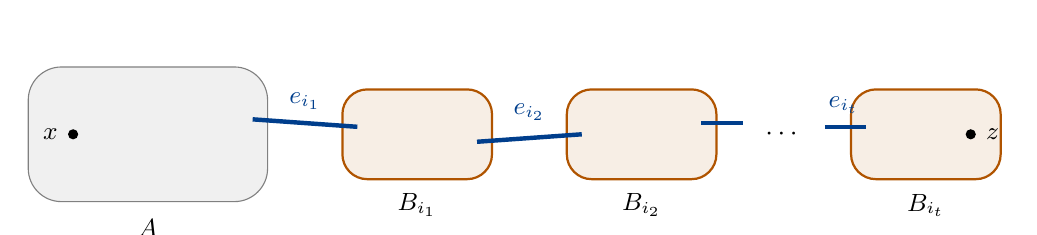
\begin{tikzpicture}[scale=0.95,
    vtx/.style={circle, fill, inner sep=1.3pt},
    piece/.style={draw=figaux, fill=figaux!10, rounded corners=9pt, thick},
    root/.style={draw=figgrey, fill=figgrey!12, rounded corners=12pt},
    seam/.style={figmain, line width=1.6pt}]
  \draw[root] (0,-0.9) rectangle (3.2,0.9);
  \node[font=\small] at (1.6,-1.25) {$A$};
  \node[vtx] (x) at (0.6,0) {};
  \node[font=\small, anchor=east] at (x.west) {$x$};
  % pieces
  \draw[piece] (4.2,-0.6) rectangle (6.2,0.6);
  \draw[piece] (7.2,-0.6) rectangle (9.2,0.6);
  \draw[piece] (11.0,-0.6) rectangle (13.0,0.6);
  \node[font=\small] at (5.2,-0.95) {$B_{i_1}$};
  \node[font=\small] at (8.2,-0.95) {$B_{i_2}$};
  \node[font=\small] at (12.0,-0.95) {$B_{i_t}$};
  \node at (10.1,0) {$\cdots$};
  % seams
  \draw[seam] (3.0,0.2) -- (4.4,0.1);
  \draw[seam] (6.0,-0.1) -- (7.4,0.0);
  \draw[seam] (9.0,0.15) -- (9.55,0.15);
  \draw[seam] (10.65,0.1) -- (11.2,0.1);
  \node[font=\small, text=figmain, anchor=south] at (3.7,0.2) {$e_{i_1}$};
  \node[font=\small, text=figmain, anchor=south] at (6.7,0.05) {$e_{i_2}$};
  \node[font=\small, text=figmain, anchor=south] at (10.9,0.15) {$e_{i_t}$};
  \node[vtx] (z) at (12.6,0) {};
  \node[font=\small, anchor=west] at (z.east) {$z$};
\end{tikzpicture}

\caption{The cluster of $x$ after the switching procedure (schematic). Each inserted piece $B_{i_j}$ is
attached to its predecessor by a single open seam $e_{i_j}$, so the seams are bridges separating $x$
from~$z$. Cutting the seams recovers $A$ and all pieces (\cref{lem:switching,lem:codes}).}\label{fig:chain}
\end{figure}

\subsection{Undoing the splicing}\label{sec:codes}

Fix $x$ and~$z$. For a configuration $\omega'$ with $z\in C_x(\omega')$, list the bridges of
$C_x(\omega')$ that separate $x$ from $z$ in their order from $z$ towards~$x$. A \emph{code} is a
sequence $c=(c_\ell,\dots,c_1)$ with entries in $\{\ast\}\cup\{1,\dots,M\}$. A successful run with output
distinguished configuration $\omega'^{(0)}$ has the following code: $c_i=\ast$ if $i$ is not selected,
and for the selected indices, read from $z$ towards $x$, the entry $c_{i_j}$ is the number of
separating bridges after the previous seam (or after $z$), up to and including $e_{i_j}$. We call
$c_{i_j}$ the \emph{gap} of $e_{i_j}$. Recall that $\sigma=1/2+\varepsilon$, and put
\begin{equation*}
  \Theta_M\coloneqq1+\sum_{m=1}^M\min\Bigl\{1,\frac{2M^\sigma}{m}\Bigr\}\le CM^\sigma\log M\,.
\end{equation*}

\begin{lemma}[Inverse codes]\label{lem:codes}
Fix $x$, $z$ and output configurations $\omega'^{(0)},\dots,\omega'^{(\ell)}$.
\begin{enumerate}[label=\textup{(\alph*)}]
  \item\label{it:codes-inverse} A code determines the input configurations, the sets $A$ and $B_i$, the
  seams, the masks and the contact sets $\mathcal K_i$ of every successful run with this output and
  this code.
  \item\label{it:codes-gaps} In every successful run each gap satisfies
  $1/\abs{\mathcal K_{i}}\le\min\{1,2M^\sigma/c_{i}\}$.
  \item\label{it:codes-sum} Summed over the codes $c$ of successful runs with this output,
  $\sum_c\prod_{i\colon c_i\neq\ast}\abs{\mathcal K_i}^{-1}\le\Theta_M^\ell$.
\end{enumerate}
\end{lemma}

\begin{proof}
\ref{it:codes-inverse}: The code locates the seams among the separating bridges. By
\cref{lem:switching}, cutting them decomposes $C_x(\omega'^{(0)})$ into $A$ (the part containing $x$)
and the pieces $B_{i_1},\dots,B_{i_t}$ in their order. This determines the set $S$ before each round,
hence every mask, and undoing the exchanges in reverse order recovers the input configurations. The
contact sets are then determined by the input configurations and the pieces.

\ref{it:codes-gaps}: The separating bridges counted in the gap of $e_i$, other than $e_i$ itself, lie
inside $B_i$, between the point where the next seam (or $z$) attaches and the endpoint of $e_i$.
Since $B_i$ is joined to the rest of the cluster by at most two edges, both of them bridges, a
self-avoiding path between two vertices of $B_i$ stays in~$B_i$; so these edges are bridges of $B_i$
separating two of its vertices.
By \cref{lem:switching} the open edges inside $B_i$ are those of~$\omega^{(i)}$. Hence
$c_i-1\le\diambr(B_i)$, the bridge diameter of $B_i$ in~$\omega^{(i)}$. Now $B_i$ is a component of the
$\omega^{(i)}$-open subgraph induced by $C_i\setminus S$, joined to $C_i\cap S$ by the
$\abs{\mathcal K_i}\ge1$ open edges of $\mathcal K_i$. Since $C_i$ is $M$-good, $\diambr(B_i)\le
\abs{\mathcal K_i}M^\sigma$. If $c_i=1$ the claim is $\abs{\mathcal K_i}\ge1$; otherwise $c_i-1\ge
c_i/2$ gives $1/\abs{\mathcal K_i}\le M^\sigma/(c_i-1)\le2M^\sigma/c_i$. Also $c_i-1\le\abs{B_i}-1$,
so $c_i\le M$ and codes indeed take values in $\{\ast\}\cup\{1,\dots,M\}$.

\ref{it:codes-sum}: By~\ref{it:codes-gaps}, the product for a code of a successful run is at most
$\prod_{i\colon c_i\neq\ast}\min\{1,2M^\sigma/c_i\}$. Summing this over all sequences
$c\in(\{\ast\}\cup\{1,\dots,M\})^\ell$ gives $\Theta_M^\ell$. The bound on $\Theta_M$ is the harmonic sum.
\end{proof}

All configurations of a successful run are determined, as far as they matter, by the edges in a fixed
finite ball around~$x$: the cluster $A$ is explored within distance $2n$, the chain moves at most $\nu$
steps from $z\in C_x(\omega'^{(0)})$, each rule reads edges within distance $r_\Phi$ of its vertex, and
every mask lies within distance one of a piece. Conditioning on all other edges, we may therefore treat
the trajectories as elements of a finite product space. On it, the exchanges preserve the total number
of open edges among the $\ell+1$ configurations, so input and output configurations have the same
probability under the product measure. This is the basis of the following density description.

\begin{lemma}[The load]\label{lem:density}
For $x,z\in V$ and a configuration $\omega$ let
\begin{equation*}
  L_x(z,\omega)\coloneqq\frac1n\,\EE\Bigl[\sum_\tau\prod_{i=1}^\ell\Phi_{y_i}(\omega^{(i)},y_{i-1})
  \prod_{j=1}^t\abs{\mathcal K_{i_j}}^{-1}\Bigr]\,,
\end{equation*}
where the expectation is over independent auxiliary configurations $\omega'^{(1)},\dots,\omega'^{(\ell)}$
with law $\PP_{p_c}$, and the sum is over the trajectories $\tau$ of successful runs whose output is
$(\omega,\omega'^{(1)},\dots,\omega'^{(\ell)})$; the factors are evaluated on these trajectories. Then,
for every event~$\mathcal B$,
\begin{equation}\label{eq:density}
  \frac1n\,\PP\bigl(\text{the experiment succeeds and }\omega'^{(0)}\in\mathcal B\bigr)
  =\EE_{p_c}\bigl[L_x(z,\omega)\1_{\mathcal B}(\omega)\bigr]\,.
\end{equation}
Moreover $0\le L_x(z,\omega)\le\Theta_M^\ell/n$; the function $L_x(z,\cdot)$ depends only on the edges in a
finite ball around~$x$; $L_{gx}(gz,g\omega)=L_x(z,\omega)$ for $g\in\Aut(G)$; and $L_x(z,\omega)=0$
unless $z\in C_x(\omega)$ and $\abs{C_x(\omega)}<2n+\nu$.
\end{lemma}

\begin{proof}
A trajectory has probability $\PP_{p_c}(\omega^{(0)})\cdots\PP_{p_c}(\omega^{(\ell)})
\prod_i\Phi_{y_i}(\omega^{(i)},y_{i-1})\prod_j\abs{\mathcal K_{i_j}}^{-1}$ on the finite product space.
The product of the configuration probabilities equals that of the output configurations. Summing over
trajectories with a given output gives~\eqref{eq:density}. For the upper bound, group the trajectories
with a given output by their codes. By \cref{lem:codes}\ref{it:codes-inverse}, the code determines the
input configurations and the seams, so for fixed code the sum over trajectories is a sum over chains,
and $\sum_{\text{chains}}\prod_i\Phi_{y_i}(\omega^{(i)},y_{i-1})\le1$ because these are the
probabilities of the chains given the input configurations. \Cref{lem:codes}\ref{it:codes-sum} bounds
the remaining sum over codes by $\Theta_M^\ell$. Locality and covariance hold because every ingredient is
defined locally and covariantly, and the support property is~\eqref{eq:switch-cluster}.
\end{proof}

\subsection{First and second moment of the load}\label{sec:load}

Let $L(\omega)\coloneqq\sum_zL_x(z,\omega)$ be the \emph{total load} and $\bar L\coloneqq\EE_{p_c}L$; by
invariance these do not depend on~$x$ in law. Write $\pi\coloneqq\pi_n$, and let
\begin{align*}
  T^{(n)}(x,y)&\coloneqq\PP_{p_c}\bigl(y\in C_x,\ n\le\abs{C_x}<2n\bigr)\,,\\
  \chi^{(n)}&\coloneqq\sum_yT^{(n)}(o,y)=\EE_{p_c}\bigl[\abs{C_o};\,n\le\abs{C_o}<2n\bigr]\,.
\end{align*}
The kernel $T^{(n)}$ is symmetric, because $y\in C_x$ implies $C_x=C_y$, and
$n\pi\le\chi^{(n)}\le2n\pi$.

\begin{lemma}[Mean load]\label{lem:mean-load}
The \emph{mean load} $\bar L(x,z)\coloneqq\EE_{p_c}L_x(z,\omega)$ is a kernel with row sums $\bar L$, and
\begin{equation}\label{eq:mean-load}
  \bar L(x,z)=\frac{s^\ell}n\sum_yT^{(n)}(x,y)\,K^\ell(z,y)\,,\qquad
  \pi s^\ell\le\bar L\le2\pi s^\ell\,,\qquad\norm{\bar L(\cdot,\cdot)}\le\bar L\,r^\ell\,.
\end{equation}
\end{lemma}

\begin{proof}
By~\eqref{eq:density}, $\bar L(x,z)$ is $1/n$ times the success probability of the experiment. The $\ell$ steps
of the chain use independent configurations, each succeeding with probability $s$ and moving according
to $K$, so the chain succeeds and ends at $y$ with probability $s^\ell K^\ell(z,y)$; independently, $y\in A$
and $n\le\abs A<2n$ with probability $T^{(n)}(x,y)$. Since $K^\ell$ is doubly stochastic,
$\bar L=\sum_z\bar L(x,z)=s^\ell\chi^{(n)}/n\in[\pi s^\ell,2\pi s^\ell]$. Finally
$\bar L(\cdot,\cdot)=(s^\ell/n)\,T^{(n)}(K^\ell)^\top$, and the Schur test gives
$\norm{T^{(n)}}\le\chi^{(n)}$, so $\norm{\bar L(\cdot,\cdot)}\le(s^\ell/n)\chi^{(n)}r^\ell=\bar Lr^\ell$.
\end{proof}

The mean kernel already has the desired small norm. To turn the load into the output probabilities of a
new map we must divide by a bound on~$L$, and we need that most of the mean is carried by
configurations on which $L$ is not much larger than its mean. This is what the second moment controls.

\begin{lemma}[Second moment of the load]\label{lem:second-moment}
There is a polynomial $Q(\ell,M)\ge1$, with coefficients depending only on~$G$, such that
\begin{equation}\label{eq:second-moment}
  \EE_{p_c}L^2\le Q(\ell,M)\,\pi s^{2\ell}\qquad\text{whenever }n\in\mathcal N,\ \ell M\le n/2\text{ and }
  n\ge(\Theta_M/s)^\ell\,.
\end{equation}
\end{lemma}

\begin{proof}
Expand $L^2=\sum_{z_1,z_2}L_x(z_1,\omega)L_x(z_2,\omega)$, using two independent families of auxiliary
output configurations. Each summand is a weighted sum over pairs $(\tau^1,\tau^2)$ of trajectories of
successful runs with the common distinguished output~$\omega$ and endpoints $z_1,z_2$. We split the pairs
into three classes. For a trajectory with at least one round, let $H^1$ or $H^2$ be its hanging part
(\cref{lem:switching}); it contains the endpoint and has at most $\nu$ vertices. Two hanging parts in the
same cluster are the far sides of bridges, so they are nested or disjoint.

\emph{Class~1: one of the trajectories has no round.} Let $L^\emptyset(\omega)$ be the part of
$L(\omega)$ coming from trajectories without rounds. For them the output equals the input, so
$A=C_x(\omega)$, $n\le\abs A<2n$, $z\in A$, and the chain from $z$ ends in~$A$. Hence
\begin{equation*}
  L^\emptyset(\omega)\le\frac{s^\ell}n\,\1\{n\le\abs{C_x(\omega)}<2n\}\sum_{z\in C_x(\omega)}\
  \sum_{y\in C_x(\omega)}K^\ell(z,y)\le\frac{s^\ell}{n}\,2n=2s^\ell\,,
\end{equation*}
using that the column sums of $K^\ell$ are one. The pairs of class~1 contribute at most
$2\EE_{p_c}[L^\emptyset L]\le4s^\ell\bar L\le8\pi s^{2\ell}$.

\emph{Class~2: the hanging parts are nested or joined by an edge of~$G$.} Fix $\tau^1$, with hanging part
$H^1\ni z_1$. We claim that at most $N_\nu\coloneqq\nu+\nu^2+d\nu^3$ endpoints $z_2$ admit a
trajectory $\tau^2$ in this class. If $H^2\subseteq H^1$, then $z_2\in H^1$: at most $\nu$ choices. If
$H^1\subsetneq H^2$, the first seam of $\tau^2$ is a bridge separating $x$ from $z_1$, and the bridges
between it and $z_1$ lie in $H^2$; so it is among the last $\nu$ such bridges, it determines $H^2$, and
$z_2\in H^2$: at most $\nu^2$ choices. If $H^1$ and $H^2$ are disjoint and joined by an edge, pick a
vertex of $H^2$ adjacent to $H^1$ (at most $d\nu$ choices); the first seam of $\tau^2$ is among the last
$\nu$ bridges separating $x$ from it, and $z_2\in H^2$: at most $d\nu^3$ choices. By
\cref{lem:density}, $L_x(z_2,\omega)\le\Theta_M^\ell/n\le s^\ell$ for each such $z_2$. Hence class~2
contributes at most $\EE_{p_c}[L]N_\nu s^\ell\le2N_\nu\pi s^{2\ell}$.

\emph{Class~3: the hanging parts are disjoint and not joined by any edge of~$G$.} Undo both
trajectories: by \cref{lem:switching} the changes of the distinguished configuration made by $\tau^a$
concern edges with an endpoint in $H^a$, and these two sets of edges are disjoint, so the undoing
operations commute. Let $\omega_{00}$ be the jointly restored distinguished configuration. We claim:
\begin{enumerate}[label=(\alph*)]
  \item $C_x(\omega_{00})=A_{00}\coloneqq C_x(\omega)\setminus(H^1\cup H^2)$, and
  $n-\nu\le\abs{A_{00}}<2n$;
  \item running the switching procedure of $\tau^1$ from $A_{00}$ instead of from
  $A^1\coloneqq C_x(\omega)\setminus H^1$, with the jointly restored configurations and the same chain
  and seams, reproduces the selected indices, pieces, contact sets and masks of~$\tau^1$; the same
  holds for~$\tau^2$. In particular, the first selected cluster of each chain meets $A_{00}$.
\end{enumerate}
For~(a): undoing $\tau^1$ alone restores the input of $\tau^1$, whose cluster of $x$ is $A^1$ by
\cref{lem:switching}; its edges to $H^1$ are closed and remain so, because undoing $\tau^2$ changes only
edges with an endpoint in $H^2$, and no edge joins $H^1$ to~$H^2$. The same holds with the roles
exchanged. Edges with both endpoints in $A_{00}$ are not changed, and $A_{00}$ is connected, because
removing the far sides of two bridges leaves the near side connected. Hence $C_x(\omega_{00})=A_{00}$.
Finally $\abs{A^1}\in[n,2n)$ and $\abs{H^2}\le\nu$.

For~(b) we argue by induction over the rounds of $\tau^1$, writing $S$ for the current set of the
original run and $S_0$ for that of the new run; initially $S_0=S\setminus H^2$, and $H^2\subseteq S$
throughout, since $H^2\subseteq A^1$. Let $i$ be the index selected in the original run and
$e_i=\{a_i,b_i\}$ its seam with $a_i\in S$ and $b_i\in B_i\subseteq H^1$. Since no edge joins $H^1$ to
$H^2$, we have $a_i\notin H^2$, so $C_i\ni a_i$ meets $S_0$, while every larger eligible index misses
$S\supseteq S_0$. Hence the same index is selected. The new piece is the component of $y_i$ in the
$\omega^{(i)}$-open subgraph on $V\setminus S_0=(V\setminus S)\cup H^2$; an open path leaving $B_i$
would have to enter $H^2$ through an edge from $B_i\subseteq H^1$, which does not exist, so the piece is
again~$B_i$. For the same reason the contact sets and the masks of the two runs coincide, and the states
exchanged on the mask agree, because undoing $\tau^2$ changed no edge with an endpoint in~$H^1$.
Afterwards $S_0\cup B_i=(S\cup B_i)\setminus H^2$. The stopping rules agree because $z_1\in H^1$ is not
in~$H^2$. The first selected cluster meets $S_0=A_{00}$ by the argument just given.

By~(b), a pair $(\tau^1,\tau^2)$ of class~3 is determined by the jointly restored configurations
together with the two chains and the two seam sequences: rerunning both procedures from $A_{00}$ and
applying their disjoint exchanges recovers the output. The exchanges preserve the total number of open
edges, so the weight of the pair equals the probability of the restored configurations, times the
chain probabilities and the factors $\prod\abs{\mathcal K}^{-1}$ of the two procedures run from
$A_{00}$. For fixed restored configurations and chains, the selected indices, the pieces and the contact
sets of each procedure do not depend on the seam choices, because every round adds the whole piece to
the current set; only the masks and the output depend on the seams. Hence the factors
$\prod\abs{\mathcal K}^{-1}$ are the probabilities of the uniform seam choices of each run, their sum
over the seam sequences of one run is one, and the sum over pairs of seam sequences is at most the
product of these two sums. Dropping
all conditions except~(a) and the fact that each chain succeeds and meets $A_{00}$, we obtain that
class~3 contributes at most
\begin{equation*}
  \frac1{n^2}\sum_{z_1,z_2}\EE_{p_c}\bigl[\1\{n-\nu\le\abs{C_x}<2n\}\,
  \mathrm{hit}_{z_1}(C_x)\,\mathrm{hit}_{z_2}(C_x)\bigr]\,,
\end{equation*}
where, for a fixed set $D$, $\mathrm{hit}_z(D)$ is the probability that a chain of $\ell$ independent
steps of $\Phi$ from $z$ succeeds and that one of its clusters $C_i$ meets~$D$. To bound it, let every
vertex $z$ send unit mass to each vertex of $C_1\cup\dots\cup C_\ell$ when its chain succeeds. A successful
chain has probability $s^\ell$ and its clusters have at most $\nu$ vertices in total, so each vertex sends
expected mass at most $\nu s^\ell$, and by the mass-transport principle each vertex receives at most
$\nu s^\ell$. A union bound over the vertices of $D$ gives
\begin{equation*}
  \sum_z\mathrm{hit}_z(D)\le\nu s^\ell\abs D\,.
\end{equation*}
Since $\nu\le n/2$, class~3 therefore contributes at most
\begin{equation*}
  \frac{\nu^2s^{2\ell}}{n^2}\,\EE_{p_c}\bigl[\abs{C_x}^2;\,n/2\le\abs{C_x}<2n\bigr]
  \le4\nu^2s^{2\ell}\,\PP_{p_c}(n/2\le\abs{C_o}<2n)\le4(1+2^\beta)\nu^2\pi s^{2\ell}\,,
\end{equation*}
by~\eqref{eq:scales}. Adding the three classes gives~\eqref{eq:second-moment} with
$Q(\ell,M)\coloneqq8+2N_\nu+10\nu^2$, since $4(1+2^\beta)\le10$.
\end{proof}

\subsection{One amplification step and the iteration}\label{sec:iteration}

By \cref{prop:good} there is $M_\varepsilon$ such that the bound of \cref{prop:good} holds for all
$M\ge M_\varepsilon$.

\begin{lemma}[One amplification step]\label{lem:one-step}
Let $\Phi$ be a local endpoint map with cap $M\ge2$, success probability $s$ and kernel norm~$r$. Let
$\ell\in\N$ and $n\in\mathcal N$ satisfy
\begin{equation}\label{eq:one-step-conditions}
  \ell M\le n/2\,,\qquad n\ge(\Theta_M/s)^\ell\,,\qquad 2n\ge M_\varepsilon\,,\qquad
  16\,Q(\ell,M)\,n^\beta\e^{-n^\varepsilon}\le1\,.
\end{equation}
Then there is a local endpoint map $\Phi'$ with cap $M'\coloneqq2n+\ell M$, success probability
$s'\ge\pi_n/(8Q(\ell,M))$ and kernel norm $r'\le2r^\ell$.
\end{lemma}

\begin{proof}
Put $b\coloneqq4Q(\ell,M)s^\ell$. By \cref{lem:mean-load,lem:second-moment},
$\EE_{p_c}[L;L>b]\le\EE_{p_c}L^2/b\le\pi s^\ell/4\le\bar L/4$. The load vanishes unless
$\abs{C_x}<2n+\nu\le M'$, so by \cref{prop:good}, $M'\ge M_\varepsilon$ and $\pi_n\ge n^{-\beta}$,
\begin{equation*}
  \EE_{p_c}\bigl[L;\,L\le b,\ C_x\text{ not $M'$-good}\bigr]\le b\,\e^{-(M')^\varepsilon}
  \le\bar L\cdot\frac{4Q(\ell,M)}{\pi_n}\,\e^{-n^\varepsilon}\le\frac{\bar L}4\,,
\end{equation*}
by the last condition in~\eqref{eq:one-step-conditions}. Let $\mathcal R$ be the event that $L\le b$
and $C_x$ is $M'$-good, and define
\begin{equation*}
  \Phi'_x(\omega,z)\coloneqq\1_{\mathcal R}(\omega)\,\frac{L_x(z,\omega)}{b}\,.
\end{equation*}
By \cref{lem:density} this is a local endpoint map with cap~$M'$: on $\mathcal R$ the outputs have total
probability $L/b\le1$, every output lies in $C_x$, and $\abs{C_x}<M'$ with $C_x$ being $M'$-good. Its
unconditional endpoint kernel $F'_{p_c}(x,z)=\EE_{p_c}[L_x(z,\omega);\mathcal R]/b$ satisfies
$0\le bF'_{p_c}(x,z)\le\bar L(x,z)$, and its row sums are $s'=\EE_{p_c}[L;\mathcal R]/b\ge\bar L/(2b)\ge\pi_n/(8Q(\ell,M))$. Hence
$r'=\norm{F'_{p_c}}/s'\le\norm{\bar L(\cdot,\cdot)}/(\bar L/2)\le2r^\ell$ by \cref{lem:kernels}\ref{it:domination}
and~\eqref{eq:mean-load}.
\end{proof}

The new map $\Phi'$ consists of fixed functions $\Phi'_x(\omega,\cdot)$ of the configuration. Like every
local endpoint map, it can be evaluated on configurations of any parameter; this is how the maps are used
in \cref{sec:moments}.

\begin{proof}[Proof of \cref{prop:amplification}]
We measure a map $\Phi$ with cap $M$ and success probability $s$ by
\begin{equation*}
  \operatorname{cost}(\Phi)\coloneqq\log(1/s)+(\sigma+\xi)\log M\,,
\end{equation*}
where $\xi>0$ is fixed so small that, by~\eqref{eq:beta-sigma},
\begin{equation*}
  c_\xi\coloneqq\frac{\beta+\xi+(\sigma+\xi)(1+\xi)}{1-\xi}<1\,.
\end{equation*}
Fix the constant $C$ in $\Theta_M\le CM^\sigma\log M$, and choose $M_1\ge M_\varepsilon$ so large that
$\log(2C\log M)\le\xi\log M$ for $M\ge M_1$. By \cref{lem:start} there is a map $\Phi_0$ with cap
$M\ge M_1$ and kernel norm $r<\e^{-1}$.

\emph{One step.} Let $\Phi$ have cap $M\ge M_1$, success probability $s$ and kernel norm
$r<\e^{-1}$, and put $a\coloneqq\lceil CM^\sigma\log M/s\rceil$. Then $a\ge\max\{2,\Theta_M/s\}$ and
$\log a\le\log(1/s)+\sigma\log M+\log(2C\log M)\le\operatorname{cost}(\Phi)$. For $n\in\mathcal N$ put
$\ell\coloneqq\lfloor\log n/\log a\rfloor$, so that $a^\ell\le n<a^{\ell+1}$. As $n\to\infty$ through
$\mathcal N$, we have $\ell\to\infty$ and $\ell\le\log n/\log2$; hence all conditions
in~\eqref{eq:one-step-conditions} hold for large~$n$, using that $Q(\ell,M)$ is polynomial in~$\ell$ and
$n\ge a^\ell\ge(\Theta_M/s)^\ell$. \Cref{lem:one-step} gives a map $\Phi'$ with cap $M'$, success
probability $s'$ and kernel norm $r'$. By $\pi_n\ge n^{-\beta}$ and
$\log n<(\ell+1)\operatorname{cost}(\Phi)$,
\begin{align*}
  \log(1/s')&\le\beta\log n+\log(8Q(\ell,M))\le\beta(\ell+1)\operatorname{cost}(\Phi)+O_M(\log(\ell+1))\,,\\
  \log M'&=\log(2n+\ell M)\le\log n+1\le(\ell+1)\operatorname{cost}(\Phi)+1\,,\\
  \log(1/r')&\ge\ell\log(1/r)-\log2\,.
\end{align*}
Since $\operatorname{cost}(\Phi)>0$ and $\log(1/r)>1$ are fixed, for $n$ large enough this gives
$\log(1/s')\le\ell(\beta+\xi)\operatorname{cost}(\Phi)$, $\log M'\le\ell(1+\xi)\operatorname{cost}(\Phi)$
and $\log(1/r')\ge\ell(1-\xi)\log(1/r)\ge2\log(1/r)$, and therefore
\begin{equation*}
  \frac{\operatorname{cost}(\Phi')}{\log(1/r')}
  \le\frac{\ell\operatorname{cost}(\Phi)\,\bigl(\beta+\xi+(\sigma+\xi)(1+\xi)\bigr)}{\ell(1-\xi)\log(1/r)}
  =c_\xi\,\frac{\operatorname{cost}(\Phi)}{\log(1/r)}\,.
\end{equation*}
Moreover $\Phi'$ has cap $M'\ge2n\ge M_1$ and $r'<\e^{-2}$.

\emph{Iteration.} Starting from $\Phi_0$ and applying the step repeatedly, we obtain maps
$\Phi_0,\Phi_1,\dots$ with kernel norms $r_j<\e^{-1}$ and
\begin{equation*}
  \frac{\operatorname{cost}(\Phi_j)}{\log(1/r_j)}\le c_\xi^j\,\frac{\operatorname{cost}(\Phi_0)}{\log(1/r_0)}
  \longrightarrow0\,.
\end{equation*}
Since $\log(1/s)+\log M\le\max\{1,(\sigma+\xi)^{-1}\}\operatorname{cost}(\Phi)$ for every map, the
efficiency ratio $\operatorname{eff}(\Phi_j)$ tends to zero.
\end{proof}

\section{Critical moments and the near-critical susceptibility}\label{sec:moments}

In this section we prove \cref{prop:efficient}, which completes the proof of \cref{thm:moments}, and
then the susceptibility bound~\eqref{eq:apriori-chi} of \cref{thm:apriori}. We assume
\cref{ass:G,ass:U} throughout. For a domain $\Lambda$, $p<p_c$ and $v\in V$ we write
\begin{equation*}
  \chi^\Lambda(v)\coloneqq\EE_p\abs{C^\Lambda_v}\,,
\end{equation*}
with $\chi^\Lambda(v)=0$ for $v\notin\Lambda$; the parameter $p$ will be clear from the context.

The strategy for \cref{prop:efficient} was described after its statement in \cref{sec:part1}. We run a
fixed efficient map slightly below $p_c$ and compare two bounds on the normalised susceptibility in the
complement of an independent cluster~$A$, evaluated at the endpoint of $\ell$ steps of the map. The upper
bound (\cref{sec:comparison}) says that one step can only multiply this quantity by a bounded factor,
up to a boundary contribution controlled by $\Delta(p)$. The lower bound says that after
$\ell\approx\log\chi(p)/\log(1/r)$ steps the endpoint has escaped from~$A$. Together they bound $\Delta(p)$
from below, which by Russo's formula controls the growth of~$\chi$ (\cref{sec:proof-efficient}).

\subsection{Two comparison lemmas}\label{sec:comparison}

For a domain $\Lambda$, $v\in\Lambda$ and $M\in\N_0$, let $B^\Lambda_{\mathrm{int}}(v,M)$ be the set of
vertices joined to $v$ by an open path in $\Lambda$ of length at most~$M$.

\begin{lemma}[Maximal susceptibility in an intrinsic ball]\label{lem:intrinsic-ball}
For every domain $\Lambda$, $v\in\Lambda$, $M\in\N_0$ and $p\in(0,p_c)$,
\begin{equation}\label{eq:intrinsic-ball}
  \EE_p\max_{z\in B^\Lambda_{\mathrm{int}}(v,M)}\chi^\Lambda(z)\le\Bigl(1+\frac{1-p}{p}\,M\Bigr)\chi^\Lambda(v)\,.
\end{equation}
\end{lemma}

\begin{proof}
For $M=0$ there is nothing to prove. Let first $\Lambda$ be finite, and let $Y=Y(\omega)$ be a maximiser
of $\chi^\Lambda$ over $B^\Lambda_{\mathrm{int}}(v,M)$, chosen by a fixed rule.

\emph{A resampling identity.} For $w\in\Lambda$, let $W\coloneqq C^\Lambda_w(\omega)$, and let
$\tilde\omega$ be obtained from $\omega$ by resampling, independently, all edges with an endpoint in~$W$.
Given $W$, the other edges keep their product law, because the event $\{C^\Lambda_w=W\}$ depends only on
the edges with an endpoint in~$W$. Hence $\tilde\omega$ has law $\PP_p$ and is independent of~$W$, and
$\PP(Y(\tilde\omega)\in W)=\sum_z\PP_p(Y=z)\,T_p^\Lambda(w,z)$. Summing over $w$ and using the symmetry of
$T^\Lambda_p$ gives
\begin{equation}\label{eq:intrinsic-identity}
  \sum_{w\in\Lambda}\PP\bigl(Y(\tilde\omega)\in C^\Lambda_w(\omega)\bigr)
  =\EE_p\,\chi^\Lambda(Y)=\EE_p\max_{z\in B^\Lambda_{\mathrm{int}}(v,M)}\chi^\Lambda(z)\,.
\end{equation}

\emph{Entering the cluster of~$w$.} If $v\notin W$ and $Y(\tilde\omega)\in W$, take a self-avoiding
$\tilde\omega$-open path in $\Lambda$ of length at most $M$ from $v$ to $Y(\tilde\omega)$, and its first
edge $\{b,a\}$ with $b\notin W$ and $a\in W$. This edge is closed in~$\omega$, since it belongs to the
boundary of the $\omega$-cluster~$W$. The part of the path before it uses only edges without an
endpoint in~$W$, which are the same in $\omega$ and $\tilde\omega$, and it has length at most $M-1$.
Let $N_w(\omega)$ be the number of edges $\{b,a\}$ with $a\in W$, $b\in\Lambda\setminus W$, such that
$b$ is joined to $v$ by an $\omega$-open path in $\Lambda\setminus W$ of length at most $M-1$; put
$N_w\coloneqq0$ if $v\in W$. Then
\begin{equation*}
  \PP\bigl(Y(\tilde\omega)\in W\bigr)\le T^\Lambda_p(v,w)+\EE_pN_w\,.
\end{equation*}

\emph{Counting the entering edges.} Let $e$ be counted by $N_w(\omega)$, and let $\omega^e$ be $\omega$
with $e$ opened. In $\omega^e$, the edge $e$ is the only open edge between $W$ and its complement, so
$v\connin{\Lambda}w$ and $e$ is a bridge separating $v$ from~$w$. Every bridge separating $v$ from $w$
that comes before $e$ lies on the path of length at most $M-1$ from $v$ to~$b$. Hence $e$ is among the
first $M$ bridges separating $v$ from $w$ in~$\omega^e$. Since $\omega$ is recovered from $\omega^e$ by
closing~$e$, each configuration $\omega'$ with $v\connin{\Lambda}w$ arises from at most $M$ pairs
$(\omega,e)$, and $\PP_p(\omega)=((1-p)/p)\,\PP_p(\omega^e)$. Therefore
$\EE_pN_w\le((1-p)/p)\,M\,T_p^\Lambda(v,w)$. Summing over $w$ and using~\eqref{eq:intrinsic-identity}
proves~\eqref{eq:intrinsic-ball} for finite~$\Lambda$.

\emph{Infinite domains.} Exhaust $\Lambda$ by finite domains containing~$v$. The susceptibilities
increase to $\chi^\Lambda$, the intrinsic balls increase to $B^\Lambda_{\mathrm{int}}(v,M)\subseteq
B(v,M)$, and the maxima increase to the maximum. Monotone convergence concludes.
\end{proof}

Recall from \cref{lem:map-basic} the unconditional endpoint kernel $F_p$ of a map and its success
probability $s_p$ at parameter~$p$, and put $K_p\coloneqq F_p/s_p$.

\begin{lemma}[A map in a deleted domain]\label{lem:map-deleted}
Let $\Phi$ be a local endpoint map with cap $M\ge2$, success probability $s>0$ and kernel norm $r<1$.
There is $p_\Phi\in[p_c/2,p_c)$ such that $s_p\ge s/2$ and $\norm{K_p}\le\e r$ for $p\in[p_\Phi,p_c)$.
Moreover, there are $Z\in[2,CM/s]$, with $C$ depending only on~$G$, and $C_\Phi<\infty$ such that for
all $p\in[p_\Phi,p_c)$, $A\subseteq V$ and $v\in V$,
\begin{equation}\label{eq:map-deleted}
  (K_pF_A)(v)\le Z\,F_A(v)+C_\Phi\,g_A(v)\,,
\end{equation}
where
\begin{equation*}
  F_A(v)\coloneqq\frac{\chi^{V\setminus A}(v)}{\chi(p)}\qquad\text{and}\qquad
  g_A(v)\coloneqq\sum_{\substack{a\in A\\\dist(v,a)\le M}}\ \sum_{b\sim a}F_A(b)\,.
\end{equation*}
\end{lemma}

The function $F_A$ is the susceptibility in the complement of~$A$, normalised by the full
susceptibility; it vanishes on~$A$. The term $g_A(v)$ collects its values at the outer boundary of $A$
near~$v$.

\begin{proof}
By \cref{lem:map-basic}, $s_p\to s$ and $\norm{F_p-F_{p_c}}\to0$ as $p\to p_c$, so
$\norm{K_p}\to\norm{K}=r$; this gives~$p_\Phi$. Fix $p\in[p_\Phi,p_c)$, $A$ and $v$. Whenever the rule at
$v$ outputs $y$, the cluster $C_v$ has at most $M$ vertices, so a self-avoiding open path $\pi$ of length
at most $M$ joins $v$ to~$y$; choose one by a fixed rule. We bound $\sum_yF_p(v,y)F_A(y)$ by splitting
according to~$\pi$.

If $\pi$ avoids $A$, then $v\notin A$ and $y\in B^{V\setminus A}_{\mathrm{int}}(v,M)$, so by
\cref{lem:intrinsic-ball} this part is at most
$\EE_p\max_{z\in B^{V\setminus A}_{\mathrm{int}}(v,M)}F_A(z)\le(1+(1-p)M/p)\,F_A(v)$. If $y\in A$, then
$F_A(y)=0$. In the remaining case $\pi$ meets $A$ and $y\notin A$. Let $\{a,b\}$ be the last edge of
$\pi$ with $a\in A$ and $b\notin A$; then $\dist(v,a)\le M$, and the segment of $\pi$ from $b$ to $y$
lies in $V\setminus A$ and has length $l\le M$. By the Harris inequality applied to the event that this
segment is open,
\begin{equation*}
  \chi^{V\setminus A}(b)\ge\EE_p\bigl[\abs{C^{V\setminus A}_y};\text{ the segment is open}\bigr]
  \ge p^l\chi^{V\setminus A}(y)\,,
\end{equation*}
so $F_A(y)\le p^{-M}F_A(b)$, and this part is at most $p^{-M}g_A(v)$. Altogether
$\sum_yF_p(v,y)F_A(y)\le(1+(1-p)M/p)F_A(v)+p^{-M}g_A(v)$. Dividing by $s_p\ge s/2$ and using
$p\ge p_c/2$ gives~\eqref{eq:map-deleted} with $Z\coloneqq\max\{2,(2/s)(1+2M/p_c)\}$ and
$C_\Phi\coloneqq(2/s)(2/p_c)^M$.
\end{proof}

\subsection{Proof of \texorpdfstring{\cref{prop:efficient}}{Proposition 3.7}}\label{sec:proof-efficient}

\begin{proof}[Proof of \cref{prop:efficient}]
\emph{Stage 1: choice of a map.} Let $\gamma\in(0,1)$. Let $C_Z$ be a constant, depending only on~$G$,
with $\log Z\le\log(1/s)+\log M+C_Z$ for the constant $Z$ of \cref{lem:map-deleted}. If a map $\Phi$
with $r<\e^{-1}$ satisfies $\operatorname{eff}(\Phi)\le(\log2)/2$, then
$\log(1/r)\ge(\log2)/\operatorname{eff}(\Phi)\ge2$, because $\log(1/s)+\log M\ge\log 2$, and
\begin{equation*}
  \frac{\log(1/s)+\log M+C_Z}{\log(1/r)-1}=\frac{\operatorname{eff}(\Phi)\log(1/r)+C_Z}{\log(1/r)-1}
  \le\Bigl(2+\frac{2C_Z}{\log2}\Bigr)\operatorname{eff}(\Phi)\,.
\end{equation*}
By hypothesis there are such maps with arbitrarily small efficiency ratio. We fix one, $\Phi$, with cap
$M\ge2$, success probability $s$ and $r<\e^{-1}$, for which the left-hand side is at most~$\gamma$. Let
$p_\Phi$, $Z$ and $C_\Phi$ be as in \cref{lem:map-deleted}, and note that $\log Z/(\log(1/r)-1)\le\gamma$.

\emph{Stage 2: an upper bound through the boundary.} Fix $p\in[p_\Phi,p_c)$ and write $\chi=\chi(p)$.
Let $A\coloneqq C_o(\hat\omega)$ for an independent configuration $\hat\omega$ with law $\PP_p$, and
size-bias it: for functions $\mathsf G$ of a vertex set put
$\Ehat[\mathsf G(A)]\coloneqq\EE_p[\abs{C_o}\,\mathsf G(C_o)]/\chi$. For each vertex $a$, exposing the
cluster $C_a$ leaves the edges without an endpoint in $C_a$ fresh, so
\begin{equation*}
  \Ehat\Bigl[\1\{a\in A\}\sum_{b\sim a}F_A(b)\Bigr]
  =\frac1{\chi^2}\sum_{b\sim a}\EE_p\bigl[\abs{C_a}\1\{o\in C_a\}\,\abs{C_b}\1\{C_b\neq C_a\}\bigr]
  \le\Delta(p)\,,
\end{equation*}
where we used that $\abs{C_b^{V\setminus C_a}}=\abs{C_b}\1\{C_b\neq C_a\}$ and, by transitivity, that
$\sum_{b\sim a}\EE_p[\abs{C_a}\abs{C_b};C_a\neq C_b]=\chi^2\Delta(p)$ for every~$a$. Hence
$\Ehat\,g_A(v)\le\abs{B(o,M)}\,\Delta(p)$ for every~$v$. Iterating~\eqref{eq:map-deleted}, using that
$K_p$ has nonnegative entries,
\begin{equation*}
  K_p^\ell F_A\le Z^\ell F_A+C_\Phi\sum_{i=0}^{\ell-1}Z^{\ell-1-i}K_p^ig_A\,.
\end{equation*}
Evaluate at $o\in A$, where $F_A(o)=0$, and take $\Ehat$; the kernel $K_p$ is deterministic and
stochastic, and $Z\ge2$. This gives
\begin{equation}\label{eq:efficient-upper}
  \Ehat\,(K_p^\ell F_A)(o)\le C_\Phi\abs{B(o,M)}\,\Delta(p)\sum_{i=0}^{\ell-1}Z^{\ell-1-i}
  \le2C_\Phi\abs{B(o,M)}\,Z^{\ell-1}\Delta(p)\,.
\end{equation}

\emph{Stage 3: a lower bound from spreading.} Exposing $A=C_o$ as before,
\begin{equation*}
  \Ehat\,(K_p^\ell F_A)(o)=\frac1{\chi^2}\sum_vK_p^\ell(o,v)\,\EE_p\bigl[\abs{C_o}\abs{C_v};\,C_o\neq C_v\bigr]\,.
\end{equation*}
Without the restriction $C_o\neq C_v$, the Harris inequality gives
$\EE_p[\abs{C_o}\abs{C_v}]\ge\chi^2$, and $K_p^\ell$ is stochastic, so the sum would be at least one. The
removed part equals, by the mass-transport principle applied to the mass
$\abs{C_z}\sum_{v\in C_z}K_p^\ell(z,v)$ sent from $z$ to every vertex of~$C_z$,
\begin{equation*}
  \sum_vK_p^\ell(o,v)\,\EE_p\bigl[\abs{C_o}^2;\,v\in C_o\bigr]
  =\EE_p\bigl[\abs{C_o}\,\langle\1_{C_o},K_p^\ell\1_{C_o}\rangle\bigr]
  \le\norm{K_p}^\ell\,\EE_p\abs{C_o}^2\le(\e r)^\ell\chi^3\,,
\end{equation*}
by \cref{lem:correlation}\ref{it:tree}. Choose $\ell\coloneqq\lceil\log(2\chi)/(\log(1/r)-1)\rceil$, so
that $(\e r)^\ell\chi=\e^{-(\log(1/r)-1)\ell}\chi\le1/2$. Then $\Ehat\,(K_p^\ell F_A)(o)\ge1/2$.

\emph{Stage 4: growth of the susceptibility.} Since $\ell-1\le\log(2\chi)/(\log(1/r)-1)$ and
$\log Z\le\gamma(\log(1/r)-1)$, we have $Z^{\ell-1}\le(2\chi)^\gamma$. Comparing
with~\eqref{eq:efficient-upper}, we obtain $\Delta(p)\ge c_\Phi\chi^{-\gamma}$ for all $p\in[p_\Phi,p_c)$, with $c_\Phi>0$ depending on the fixed map. By \cref{lem:russo},
$(1-p)\chi'=\chi^2\Delta(p)\ge c_\Phi\chi^{2-\gamma}$ for almost every such~$p$. Hence the locally
absolutely continuous function $\chi^{-(1-\gamma)}$ has derivative at most $-(1-\gamma)c_\Phi$ almost
everywhere on $[p_\Phi,p_c)$. Integrating from $p$ to $p'<p_c$ and letting $p'\uparrow p_c$ gives
$\chi(p)^{-(1-\gamma)}\ge(1-\gamma)c_\Phi(p_c-p)$. Since $\chi$ is bounded on $[0,p_\Phi]$, we conclude
that for every $\gamma\in(0,1)$ there is $C_\gamma$ with
\begin{equation}\label{eq:efficient-chi}
  \chi(p)\le C_\gamma\,(p_c-p)^{-1/(1-\gamma)}\qquad\text{for all }p\in[0,p_c)\,.
\end{equation}

\emph{Stage 5: the critical tail.} Let $N\in\N$ be large and $p\coloneqq p_c-N^{-1/2}$. Explore $C_o$ in
a fixed order, testing each edge at most once, until the cluster is exhausted or $N$ vertices have been
found. This uses at most $dN$ tests, and the record of the exploration decides the event
$\{\abs{C_o}\ge N\}$. Let $\mathcal L_N$ be the likelihood ratio of the record under $\PP_{p_c}$ with
respect to~$\PP_p$; each test contributes a factor $p_c/p$ if the edge is open and $(1-p_c)/(1-p)$ if it
is closed. For $b>1$, the conditional $b$-th moment of one such factor under $\PP_p$ is
\begin{equation*}
  \varphi_b(p)\coloneqq p\Bigl(\frac{p_c}p\Bigr)^b+(1-p)\Bigl(\frac{1-p_c}{1-p}\Bigr)^b
  \le1+C_b(p_c-p)^2\,,
\end{equation*}
because $\varphi_b$ is smooth near the interior point $p_c$, with $\varphi_b(p_c)=1$ and
$\varphi_b'(p_c)=0$. Conditioning successively on the at most $dN$ tests gives
$\EE_p\mathcal L_N^b\le(1+C_b/N)^{dN}\le\e^{dC_b}$. By Hölder's and Markov's inequalities,
\begin{equation*}
  \PP_{p_c}(\abs{C_o}\ge N)=\EE_p\bigl[\mathcal L_N\1\{\abs{C_o}\ge N\}\bigr]
  \le\e^{dC_b/b}\,\Bigl(\frac{\chi(p)}{N}\Bigr)^{1-1/b}\,.
\end{equation*}
By~\eqref{eq:efficient-chi}, $\chi(p)\le C_\gamma N^{1/(2(1-\gamma))}$, so
$\PP_{p_c}(\abs{C_o}\ge N)\le C_{\gamma,b}N^{-\alpha'}$ with
$\alpha'\coloneqq(1-1/b)(1-1/(2(1-\gamma)))$. Given $\alpha\in(0,1/2)$, choose $\gamma$ small and $b$
large such that $\alpha'>\alpha$. Then
\begin{equation*}
  \EE_{p_c}\abs{C_o}^\alpha=\sum_{N\ge0}\bigl((N+1)^\alpha-N^\alpha\bigr)\PP_{p_c}(\abs{C_o}>N)
  \le1+C\sum_{N\ge1}N^{\alpha-1-\alpha'}<\infty\,.\qedhere
\end{equation*}
\end{proof}

\subsection{The near-critical susceptibility}\label{sec:chi}

We now prove the susceptibility bound~\eqref{eq:apriori-chi}. Its source is the following covariance
inequality for functions determined by an algorithm, due to O'Donnell, Saks, Schramm and
Servedio~\cite[Section~3.3, Equation~(6)]{OSSS05}; we include a proof in \cref{app:osss}.

\begin{lemma}[Decision-tree covariance inequality]\label{lem:osss}
Let $X=(X_i)_{i\in I}$ be a finite family of independent random variables, each taking finitely many
values, let $g=g(X)$ take values in
$[0,1]$, and let an algorithm, possibly using independent randomness, determine $g(X)$ by querying the
coordinates of $X$ one at a time, never the same coordinate twice. Let $\operatorname{rev}_i$, the
\emph{revealment} of~$i$, be the probability that coordinate $i$ is queried, and let $X^{(i)}$ be $X$ with $X_i$ replaced by an independent copy.
Then, for every real function $f$,
\begin{equation*}
  \abs{\Cov(f(X),g(X))}\le\sum_{i\in I}\operatorname{rev}_i\,\EE\abs{f(X)-f(X^{(i)})}\,.
\end{equation*}
\end{lemma}

\begin{proof}[Proof of~\eqref{eq:apriori-chi}]
Fix $\alpha\in(0,1/2)$ and put $C_\alpha\coloneqq\EE_{p_c}\abs{C_o}^\alpha$, which is finite by \cref{thm:moments}.
Let $\Lambda$ be a finite domain, $v\in\Lambda$, $n\ge2$ and $p\in(0,p_c]$. Let
$f\coloneqq\1\{\abs{C_v^\Lambda}\ge n\}$ and $\Psi(p)\coloneqq\PP_p(\abs{C_v^\Lambda}\ge n)$. Independently,
mark every vertex of $\Lambda$ with probability $1/n$, and let $g$ be the indicator that $C_v^\Lambda$
contains a mark. An algorithm that reveals all marks and then explores the clusters in $\Lambda$ of all
marked vertices determines~$g$. It queries an edge only if one of its endpoints lies in the cluster of a
marked vertex, which for a given vertex $x$ has probability
\begin{equation*}
  \EE_p\bigl[1-(1-1/n)^{\abs{C_x^\Lambda}}\bigr]\le\EE_p\min\{1,\abs{C_x^\Lambda}/n\}
  \le n^{-\alpha}\EE_p\abs{C_x^\Lambda}^\alpha\le C_\alpha n^{-\alpha}\,,
\end{equation*}
by monotonicity in $p$ and in the domain. Thus every edge has revealment at most $2C_\alpha n^{-\alpha}$. The marks
do not influence~$f$, and for an edge $e$ the increasing indicator $f$ satisfies
$\EE\abs{f(X)-f(X^{(e)})}=2p(1-p)\PP_p(e\text{ is pivotal for }f)$. By \cref{lem:osss} and Russo's
formula $\Psi'(p)=\sum_e\PP_p(e\text{ is pivotal for }f)$ on the finite domain,
\begin{equation*}
  \Cov(f,g)\le4p(1-p)\,C_\alpha n^{-\alpha}\Psi'(p)\le C_\alpha n^{-\alpha}\Psi'(p)\,.
\end{equation*}
On the other hand, conditionally on the configuration, $g=1$ with probability at least $1-(1-1/n)^n$
on $\{f=1\}$, and $\EE g\le C_\alpha n^{-\alpha}$, so $\Cov(f,g)\ge\Psi(p)\bigl(1-(1-1/n)^n-C_\alpha n^{-\alpha}\bigr)\ge\Psi(p)/2$
for $n\ge n_\alpha$. Hence $\Psi'(p)\ge c_\alpha n^\alpha\Psi(p)$ on $(0,p_c]$, and integrating from $p$ to $p_c$,
\begin{equation*}
  \PP_p\bigl(\abs{C_v^\Lambda}\ge n\bigr)\le\Psi(p_c)\,\e^{-c_\alpha(p_c-p)n^\alpha}\le C_\alpha n^{-\alpha}\e^{-c_\alpha(p_c-p)n^\alpha}\,,
\end{equation*}
where $\Psi(p_c)\le\PP_{p_c}(\abs{C_o}\ge n)\le C_\alpha n^{-\alpha}$. Letting $\Lambda\uparrow V$, which is legitimate
because $\{\abs{C_v}\ge n\}$ has a finite witness, we obtain for $\delta=p_c-p$ and all $n\ge1$
\begin{equation*}
  \PP_p(\abs{C_o}\ge n)\le C'_\alpha n^{-\alpha}\e^{-c_\alpha\delta n^\alpha}\,,\qquad
  C'_\alpha\coloneqq\max\bigl\{C_\alpha,\,n_\alpha^\alpha\e^{c_\alpha n_\alpha^\alpha}\bigr\}\,,
\end{equation*}
where the second term of the maximum covers the finitely many $n<n_\alpha$. The function
$y\mapsto y^{-\alpha}\e^{-c_\alpha\delta y^\alpha}$ is decreasing on $(0,\infty)$, and the substitution
$y=(c_\alpha\delta)^{-1/\alpha}z$ gives
\begin{equation*}
  \chi(p)=\sum_{n\ge1}\PP_p(\abs{C_o}\ge n)\le C'_\alpha\int_0^\infty y^{-\alpha}\e^{-c_\alpha\delta y^\alpha}\dd y
  =C''_\alpha\,\delta^{-(1-\alpha)/\alpha}
\end{equation*}
with $C''_\alpha\coloneqq C'_\alpha c_\alpha^{-(1-\alpha)/\alpha}\int_0^\infty z^{-\alpha}\e^{-z^\alpha}\dd z$, which is finite because
$\alpha<1$. For $\alpha=1/(2+\eta)$ we have $(1-\alpha)/\alpha=1+\eta$, which
proves~\eqref{eq:apriori-chi}.
\end{proof}

\section{The triangle diagram}\label{sec:triangle}

In this section we prove the triangle bound~\eqref{eq:apriori-triangle} of \cref{thm:apriori}. We assume
\cref{ass:G,ass:U}, fix $p\in[p_c/2,p_c)$ and write $T=T_p$ and $\delta=p_c-p$. By
\cref{lem:subcritical} the operator $T$ is bounded and positive semidefinite, and
$\nabla_p=\tr(T^3)\ge T(o,o)^3=1$.

By Russo's formula, the derivative of $\nabla_p$ is a sum over pairs of distinct clusters, weighted by
the number of edges between them and by a kernel built from~$T$. We split this sum according to the size
of the smaller cluster. If it is small, the weight is bounded by its size times~$\nabla_p$. If both
clusters are large, we use that two distinct large clusters have few edges between them: comparing an
exploration of one cluster with an exploration of the same cluster after deleting the other, the
difference of their centred scores is exactly minus $p$ times the number of these (closed) edges, and
both scores are concentrated (\cref{lem:contacts}). Together with the a priori bound on $\chi(p)$ this
yields a differential inequality for $\nabla_p$ whose solution grows more slowly than every power of
$1/\delta$.

\paragraph{Sums over pairs of clusters.}
For a nonnegative function $F$ of ordered pairs of distinct finite vertex sets, invariant under
automorphisms, put
\begin{equation*}
  \mathcal S(F)\coloneqq\EE_p\Bigl[\frac1{\abs{C_o}}\sum_{B\neq C_o}F(C_o,B)\Bigr]\,,
\end{equation*}
where the sum runs over the clusters $B$ other than~$C_o$. This is a positive linear functional, so it
satisfies the Cauchy--Schwarz inequality $\mathcal S(F_1F_2)\le\mathcal S(F_1^2)^{1/2}\mathcal S(F_2^2)^{1/2}$.
For a nonnegative invariant kernel~$\mathsf J$, recall $\mathsf J(A,B)=\sum_{a\in A,b\in B}\mathsf J(a,b)$. The mass-transport
principle gives the \emph{rerooting formula}
\begin{equation}\label{eq:reroot}
  \mathcal S\bigl(\mathsf J(A,B)\,F(A,B)\bigr)=\EE_p\Bigl[\sum_v\mathsf J(o,v)\,F(C_o,C_v)\,\1\{C_o\neq C_v\}\Bigr]\,:
\end{equation}
send from $x$ to each $y\in C_x$ the mass $\abs{C_x}^{-1}\sum_v\mathsf J(y,v)F(C_x,C_v)\1\{C_x\neq C_v\}$; the
expected mass sent out by $o$ is the left-hand side, and the expected mass received is the right-hand
side. Sending $F(A,B)/(\abs A\abs B)$ from every vertex of $A$ to every vertex of $B$ shows in the same
way that $\mathcal S(F)=\mathcal S(F^\top)$, where $F^\top(A,B)\coloneqq F(B,A)$.

\begin{lemma}[Edges between two large clusters]\label{lem:contacts}
Let $\alpha\in(0,1/2)$ and $\varepsilon_1>0$ with $\kappa\coloneqq1/2+\varepsilon_1-2\alpha<0$. There
is $C<\infty$ such that for all $p\in[p_c/2,p_c)$ and $n_0\ge1$,
\begin{equation}\label{eq:contacts}
  \mathcal S\bigl(\Adj(A,B)^2\,\1\{\min(\abs A,\abs B)\ge n_0\}\bigr)\le C\,n_0^\kappa\,.
\end{equation}
\end{lemma}

\begin{proof}
Fix an edge $\{x,v\}$ and a real number $n\ge1$, and let
$\mathcal H_n\coloneqq\{C_x\neq C_v,\ n\le\min(\abs{C_x},\abs{C_v})<2n\}$.

\emph{Stage 1: probability of two large clusters.} On $\mathcal H_n$ the events $\{\abs{C_x}\ge n\}$ and
$\{\abs{C_v}\ge n\}$ have disjoint finite witnesses, namely trees in the two distinct clusters. By the
van den Berg--Kesten inequality, monotonicity in~$p$ and Markov's inequality,
\begin{equation*}
  \PP_p(\mathcal H_n)\le\PP_{p_c}(\abs{C_o}\ge n)^2\le C n^{-2\alpha}\,,
\end{equation*}
using \cref{thm:moments}.

\emph{Stage 2: two explorations.} Explore $C_v$ in the full graph, testing every edge incident to a
discovered vertex exactly once (including edges between two discovered vertices), and stop after
$N\coloneqq\lceil2dn\rceil$ tests if the exploration has not finished. Let $S_1$ be the sum of
$\omega(e)-p$ over the tested edges. Every test is a fresh Bernoulli variable given the past, so by the
Azuma--Hoeffding inequality $\PP_p(\abs{S_1}>n^{1/2+\varepsilon_1})\le2\exp(-2n^{1+2\varepsilon_1}/N)$,
without any conditioning on the sizes.
Second, on the same configuration, expose $A\coloneqq C_x$ together with the states of its internal and
boundary edges; if $v\notin A$, explore the cluster of $v$ in $V\setminus A$ in the same way, with the
same cap~$N$, and let $S_2$ be its score ($S_2\coloneqq0$ if $v\in A$). Given the exposure, the tested
edges are fresh, so the same tail bound holds for~$S_2$.

On $\mathcal H_n\cap\{\abs{C_v}\le\abs{C_x}\}$, the cluster $B\coloneqq C_v$ has fewer than $2n$
vertices and fewer than $N$ incident edges, so both explorations finish. The first tests all edges
incident to~$B$, the second those that have no endpoint in~$A$. The difference consists of the edges
between $A$ and~$B$, all of which are closed, so
\begin{equation*}
  S_1-S_2=-p\,\Adj(A,B)\,.
\end{equation*}
Hence, on this event, $\Adj(A,B)>2n^{1/2+\varepsilon_1}/p$ forces $\abs{S_1}>n^{1/2+\varepsilon_1}$ or
$\abs{S_2}>n^{1/2+\varepsilon_1}$. Using $p\ge p_c/2$ and $N\le3dn$, and exchanging the roles of $x$ and
$v$ for the other size order, we obtain
\begin{equation*}
  \PP_p\bigl(\mathcal H_n,\ \Adj(C_x,C_v)>4n^{1/2+\varepsilon_1}/p_c\bigr)\le C\e^{-cn^{2\varepsilon_1}}\,.
\end{equation*}
The two scores are concentrated separately; no independence between them is used.

\emph{Stage 3: summation.} Since $\Adj(C_x,C_v)\le d\min(\abs{C_x},\abs{C_v})<2dn$ on $\mathcal H_n$,
Stages~1 and~2 give
$\EE_p[\Adj(C_x,C_v)\1_{\mathcal H_n}]\le Cn^{1/2+\varepsilon_1-2\alpha}+Cn\e^{-cn^{2\varepsilon_1}}
\le Cn^\kappa$. By the rerooting formula~\eqref{eq:reroot} with $\mathsf J=\Adj$, the left-hand side
of~\eqref{eq:contacts} equals
$\EE_p[\sum_{v\sim o}\Adj(C_o,C_v)\1\{\min(\abs{C_o},\abs{C_v})\ge n_0,\ C_o\neq C_v\}]$. Splitting the
minimum into the ranges $[2^in_0,2^{i+1}n_0)$, $i\ge0$, bounds it by $d\sum_{i\ge0}C(2^in_0)^\kappa\le
Cn_0^\kappa$, because $\kappa<0$.
\end{proof}

\begin{proof}[Proof of~\eqref{eq:apriori-triangle}]
\emph{Stage 1: the derivative.} Put $\mathsf J\coloneqq T^2$, a bounded, invariant, symmetric kernel. By
\cref{lem:russo} the map $p\mapsto T_p$ is locally absolutely continuous in operator norm; the trace is
cyclic by \cref{lem:trace}\ref{it:trace-cyclic} and satisfies $\abs{\tr S}\le\norm S$
(\cref{sec:mtp}). Hence $\nabla_p=\tr(T^3)$ is
locally absolutely continuous on $(0,p_c)$, with $\nabla_p'=3\tr(T^2T')$ almost everywhere. By
\eqref{eq:russo-kernel} and the rerooting formula with $F=\Adj$,
\begin{equation}\label{eq:triangle-derivative}
  (1-p)\nabla_p'=3\sum_v\mathsf J(o,v)\,\EE_p\bigl[\Adj(C_v,C_o)\1\{C_v\neq C_o\}\bigr]
  =3\,\mathcal S\bigl(\mathsf J(A,B)\Adj(A,B)\bigr)\,.
\end{equation}

\emph{Stage 2: a square bound.} By~\eqref{eq:reroot}, expanding the second factor $\mathsf J(C_o,C_v)$,
\begin{equation*}
  \mathcal S\bigl(\mathsf J(A,B)^2\bigr)=\sum_{v,x',y'}\mathsf J(o,v)\,\mathsf J(x',y')\,
  \PP_p\bigl(o\conn x',\ v\conn y',\ C_o\neq C_v\bigr)\,.
\end{equation*}
The two connections occur disjointly, so the van den Berg--Kesten inequality bounds the probability by
$T(o,x')T(v,y')$. By symmetry of $\mathsf J$ and~$T$, the resulting sum is $\tr(T\mathsf J T\mathsf J)=\tr(T^6)$, and
\cref{lem:trace}\ref{it:trace-positive} with the positive operator $T^3$ gives
\begin{equation}\label{eq:square-bound}
  \mathcal S\bigl(\mathsf J(A,B)^2\bigr)\le\tr(T^6)\le\norm{T}^3\,\nabla_p\,.
\end{equation}

\emph{Stage 3: splitting by size.} Fix $\alpha\in(0,1/2)$, $\varepsilon_1>0$ with $\kappa<0$ as in
\cref{lem:contacts}, and a size $n_0\ge1$. For the pairs in which $A=C_o$ has fewer than $n_0$ vertices,
reroot the factor $\Adj$ with~\eqref{eq:reroot} and expose~$A$. If $v\notin A$, the cluster $C_v$ is
the cluster of $v$ in $V\setminus A$, which is fresh, so
\begin{equation*}
  \EE_p\bigl[\mathsf J(A,C_v)\given A\bigr]\le\sum_{y\in A}\sum_z\mathsf J(y,z)\,T(v,z)=\sum_{y\in A}T^3(y,v)\le\abs A\,\nabla_p\,,
\end{equation*}
by \cref{lem:trace}\ref{it:trace-diagonal} for the positive operator $T^3$. Hence, using
$\abs A\1\{\abs A<n_0\}\le n_0^{1-\alpha}\abs A^\alpha$ and \cref{thm:moments},
\begin{equation*}
  \mathcal S\bigl(\mathsf J(A,B)\Adj(A,B)\1\{\abs A<n_0\}\bigr)\le d\,\nabla_p\,\EE_p\bigl[\abs{C_o};\abs{C_o}<n_0\bigr]
  \le C\,n_0^{1-\alpha}\,\nabla_p\,.
\end{equation*}
Since $\mathsf J(A,B)\Adj(A,B)$ is symmetric in $A$ and $B$ and $\mathcal S(F)=\mathcal S(F^\top)$, the same
bound holds for the pairs with $\abs B<n_0$. For the remaining pairs, the Cauchy--Schwarz inequality,
\eqref{eq:contacts} and~\eqref{eq:square-bound} give
\begin{equation*}
  \mathcal S\bigl(\mathsf J(A,B)\Adj(A,B)\1\{\min(\abs A,\abs B)\ge n_0\}\bigr)
  \le C\,n_0^{\kappa/2}\,\norm{T}^{3/2}\,\nabla_p^{1/2}\,.
\end{equation*}

\emph{Stage 4: the differential inequality.} The factor $(1-p)^{-1}$ in~\eqref{eq:triangle-derivative}
is bounded. Since $\nabla_p\ge1$, the function $\mathsf b\coloneqq\nabla_p^{1/2}$ is locally absolutely
continuous, and by Stages~1 and~3, for almost every $p\in[p_c/2,p_c)$,
\begin{equation}\label{eq:triangle-ode}
  \mathsf b'\le C\,n_0^{1-\alpha}\,\mathsf b+C\,n_0^{\kappa/2}\norm{T}^{3/2}\,.
\end{equation}

\emph{Stage 5: choice of exponents.} Let $\eta>0$, and fix $\varepsilon_2\in(0,\min\{1,\eta\})$. Choose
$\alpha<1/2$ and $\varepsilon_1,\eta'>0$ such that $\kappa<0$ and
\begin{equation*}
  A_\star\coloneqq(2-\varepsilon_2)(1-\alpha)<1\,,\qquad
  B_\star\coloneqq(2-\varepsilon_2)\bigl(\tfrac14+\tfrac{\varepsilon_1}2-\alpha\bigr)+\tfrac32(1+\eta')<1+\tfrac\eta2\,.
\end{equation*}
This is possible by continuity, because at $\alpha=1/2$ and $\varepsilon_1=\eta'=0$ the two expressions
equal $1-\varepsilon_2/2$ and $1+\varepsilon_2/4$. Take $n_0\coloneqq\delta^{-(2-\varepsilon_2)}\ge1$. By~\eqref{eq:apriori-chi},
$\norm T\le\chi(p)\le C\delta^{-1-\eta'}$, and since $\kappa/2=1/4+\varepsilon_1/2-\alpha$,
inequality~\eqref{eq:triangle-ode} becomes
\begin{equation*}
  \mathsf b'(p)\le C\,(p_c-p)^{-A_\star}\,\mathsf b(p)+C\,(p_c-p)^{-B_\star}\,.
\end{equation*}
Since $A_\star<1$, the coefficient of $\mathsf b$ is integrable on $[p_c/2,p_c)$, and the integrating
factor is bounded above and below. Hence
\begin{equation*}
  \mathsf b(p)\le C\Bigl(\mathsf b(p_c/2)+\int_{p_c/2}^p(p_c-p')^{-B_\star}\dd p'\Bigr)\le C_\eta\,\delta^{-\eta/2}\,,
\end{equation*}
where the last step uses $B_\star<1+\eta/2$. Squaring gives $\nabla_p\le C_\eta\delta^{-\eta}$.
\end{proof}

\section{The corridor deformation}\label{sec:deformation}

In this section we prove \cref{prop:deformation}. We assume \cref{ass:G,ass:U} and fix
$p\in[p_c/2,p_c)$, $q=1-p$ and $k\ge3$; only the deformation time $t\ge0$ varies. We use the notation of
\cref{def:deformation} and write $T\coloneqq T_p$ and $\chi\coloneqq\chi(p)$. All constants depend only
on~$G$; in particular they are uniform in~$p\in[p_c/2,p_c)$ and in~$k$.

The section follows the order of \cref{prop:deformation}. After some bookkeeping
(\cref{lem:deformation-basic}) we identify the corridor event and its probability
(\cref{lem:calibration}), which gives the norm bound~\ref{it:def-norm} at once. The rate
bound~\ref{it:def-rate} needs three ingredients: the deletion estimate~\ref{it:def-deletion}, a lower
bound for the mass of two distinct clusters (\cref{lem:two-clusters}), and the factorisation of the
penalty of a connection through a corridor into the penalties of its two legs (\cref{lem:two-legs}).
Item~\ref{it:def-path} is proved last.

\subsection{Bookkeeping}\label{sec:deformation-basic}

\begin{lemma}[Basic bounds and monotonicity]\label{lem:deformation-basic}
Let $D_1\coloneqq(2/p_c)(1-p_c)^{-d}$, $C_0\coloneqq\max\{\log D_1+1,\,1+2d/p_c\}$ and
$c_k\coloneqq\e^{C_0k}$. Then the following holds.
\begin{enumerate}[label=\textup{(\roman*)}]
  \item\label{it:weight-edge} For every edge $e$, $\sum_wc(w)\le c_k/k$, where the sum runs over all
  templates $w$, of any base, such that $e$ is an edge of~$\gamma_w$.
  \item\label{it:penalty-size} If $x\connin{\Lambda}y$, then $N^\Lambda_{xy}\le c_k\abs{C^\Lambda_x}$.
  \item\label{it:monotone-W} For fixed $t$, $W^\Lambda_t(x,y)$ does not decrease when edges are opened
  or when $\Lambda$ is enlarged.
\end{enumerate}
Moreover, \cref{prop:deformation}\ref{it:def-basic} holds, and for every domain $\Lambda$, all
$t\ge0$ and all $x,y\in V$
\begin{equation*}
  -\frac{\d}{\d t}\chi^\Lambda_t(x)=\EE_p\sum_yN^\Lambda_{xy}W^\Lambda_t(x,y)\,,\qquad
  -\frac{\d}{\d t}\EE_pW^\Lambda_t(x,y)=\EE_p\bigl[N^\Lambda_{xy}W^\Lambda_t(x,y)\bigr]\,.
\end{equation*}
\end{lemma}

\begin{proof}
\ref{it:weight-edge}: A template has $\abs{\gamma_w}\le k$ and $\abs{\Bl_w}\le dk$, so
$p^{-\abs{\gamma_w}}q^{-\abs{\Bl_w}}\le D_1^k$, because $p\ge p_c/2$ and $q\ge1-p_c$. Every edge of
$\gamma_w$ is traversed by~$w$. Summed over all bases, the probability that a lazy walk traverses
$e=\{a,b\}$ at its $i$-th step is $\sum_u(P^{i-1}(u,a)P(a,b)+P^{i-1}(u,b)P(b,a))=1/d$, by symmetry of~$P$. A
union bound over the $k$ steps gives $\sum_wc(w)\le D_1^kk/d$, which is at most
$D_1^k\e^k/k\le\e^{C_0k}/k$, since $k^2\le\e^k$.

\ref{it:penalty-size}: An edge that is pivotal for $x\connin{\Lambda}y$ lies on every self-avoiding
open path from $x$ to $y$ in~$\Lambda$. Fix one such path; it has fewer than $\abs{C^\Lambda_x}$ edges,
and every counted template contains one of them. Apply~\ref{it:weight-edge}.

\ref{it:monotone-W}: Let the configuration or the domain grow, and suppose $x$ and $y$ were already
connected before; otherwise there is nothing to prove. Every self-avoiding open path from $x$ to $y$
before the change is still one afterwards. Hence an edge that is pivotal afterwards lies on all old
paths, so it was open and pivotal before, and the loop-erased path of a template counted afterwards
was contained in the old domain. A blocker that is closed or outside the domain afterwards was so
before. Thus every template counted afterwards was counted before, with the same weight, and
$N^\Lambda_{xy}$ cannot increase.

For \cref{prop:deformation}\ref{it:def-basic}: the counting condition is symmetric in $x$ and $y$, and
all definitions are covariant, so $T_t$ is symmetric and invariant; $0\le W^V_t\le\1\{x\conn y\}$ gives
$0\le T_t\le T$ and $\chi_t\le\chi$; and the Schur test gives $\norm{T_t}\le\chi_t$, the row sum. By
\ref{it:penalty-size}, $\sum_yN^\Lambda_{xy}W^\Lambda_t(x,y)\le c_k\abs{C_x}^2$, whose expectation is at
most $c_k\chi^3$ by \cref{lem:correlation}\ref{it:tree}; for a single entry the bound
$N^\Lambda_{xy}W^\Lambda_t(x,y)\le c_k\abs{C^\Lambda_x}$ suffices. Dominated convergence therefore
justifies differentiating $W^\Lambda_t(x,y)=\1\{x\connin{\Lambda}y\}\e^{-tN^\Lambda_{xy}}$ under the
expectation and the sum, and shows that the derivatives are continuous in~$t$.
\end{proof}

\subsection{The corridor event}\label{sec:calibration}

Recall that for a template $w$ with base $u=w_0$ and end $v=w_k$, the interior $I_w$ consists of the
vertices of $\gamma_w$ other than $u$ and~$v$, and $\Lambda_w=V\setminus I_w$.

\begin{lemma}[The corridor event]\label{lem:calibration}
Let $w$ be a template with base $u$ and end~$v$.
\begin{enumerate}[label=\textup{(\alph*)}]
  \item\label{it:cal-indep} The event $\Cor_w$ depends only on the edges incident to $I_w$; in particular
  it is independent of the states of the edges with both endpoints in~$\Lambda_w$.
  \item\label{it:cal-weight} $c(w)\,\PP_p(\Cor_w)=\mu(w)$.
  \item\label{it:cal-counted} On $\Cor_w$, the template $w$ is counted for $(x,y)$ in $V$ if and only if
  $C_u^{\Lambda_w}\neq C_v^{\Lambda_w}$ and either $x\in C_u^{\Lambda_w}$ and $y\in C_v^{\Lambda_w}$, or
  $x\in C_v^{\Lambda_w}$ and $y\in C_u^{\Lambda_w}$.
\end{enumerate}
\end{lemma}

\begin{proof}
Every edge of $\gamma_w$ has an endpoint in $I_w$ because $\abs{\gamma_w}\ge3$, and the blockers are the
other edges incident to~$I_w$; this gives~\ref{it:cal-indep}. The event $\Cor_w$ prescribes
$\abs{\gamma_w}$ open and $\abs{\Bl_w}$ closed edges, which gives~\ref{it:cal-weight}.

For~\ref{it:cal-counted}, note that on $\Cor_w$ every interior vertex has exactly two open edges, the
corridor edges (\cref{fig:corridor}). Suppose $w$ is counted for $(x,y)$. If $x\in I_w$, a
self-avoiding open path starting at $x$ uses only one of the two corridor edges at~$x$, so the other one
is not pivotal; hence $x\notin I_w$, and likewise $y\notin I_w$. A self-avoiding open path from $x$ to $y$ uses all corridor
edges, so it runs through the whole corridor, from $u$ to $v$ or from $v$ to~$u$, and its two remaining
parts lie in $\Lambda_w$. If $C_u^{\Lambda_w}=C_v^{\Lambda_w}$, an open path from $u$ to $v$ in
$\Lambda_w$ would bypass the corridor, so its edges would not be pivotal. This proves one direction.
Conversely, if the two exterior clusters are distinct and contain $x$ and $y$ as stated, then the
corridor is the only open link between them, so all its edges are open and pivotal for $x\conn y$, and
all blockers are closed.
\end{proof}

\begin{proof}[Proof of \cref{prop:deformation}\ref{it:def-norm}]
By \cref{lem:deformation-basic} with $\Lambda=V$, $-\partial_tT_t(x,y)=\EE_p[N^V_{xy}W^V_t(x,y)]\le\EE_pN^V_{xy}=\sum_w
c(w)\,\PP_p(w\text{ is counted for }(x,y))$. By \cref{lem:calibration}, a counted template requires
$\Cor_w$ and one of two exterior events, which are independent of~$\Cor_w$. In each exterior event the
connections from $x$ and from $y$ lie in distinct clusters, so they occur disjointly, and the
van den Berg--Kesten inequality and $T^{\Lambda_w}\le T$ bound its probability by $T(x,u)T(v,y)$,
respectively $T(x,v)T(u,y)$. With $c(w)\PP_p(\Cor_w)=\mu(w)$, adding the raw paths that are not
templates, and summing over raw paths with base $u$ and end $v$, which gives $P^k(u,v)$, we obtain
\begin{equation*}
  -\partial_tT_t(x,y)\le\sum_{u,v}P^k(u,v)\bigl(T(x,u)T(v,y)+T(x,v)T(u,y)\bigr)=2\,(TP^kT)(x,y)\,,
\end{equation*}
by symmetry of~$P^k$. Integrating, $0\le T-T_t\le2t\,TP^kT$ entrywise. By
\cref{lem:kernels}\ref{it:domination}, $\norm{T-T_t}\le2t\norm{TP^kT}\le2t\rho^k\norm{T}^2$, and the
triangle inequality gives~\ref{it:def-norm}. No positivity of $T_t$ is used.
\end{proof}

\subsection{Deletion and the rate bound}\label{sec:rate}

\begin{proof}[Proof of \cref{prop:deformation}\ref{it:def-deletion}]
Fix a configuration and $y$, and suppose that $W^\Lambda_t(z,y)>W^{\Lambda\setminus A}_t(z,y)$; recall
that $W^{\Lambda\setminus A}_t\le W^\Lambda_t$ by \cref{lem:deformation-basic}\ref{it:monotone-W}. We
claim that some self-avoiding open path from $z$ to $y$ in $\Lambda$ visits~$\Nb[A]$. If
$z\connin{\Lambda\setminus A}y$ fails, every open path from $z$ to $y$ in $\Lambda$ visits~$A$.
Otherwise some template $w$ is counted for $(z,y)$ in $\Lambda\setminus A$ but not in~$\Lambda$. Its
loop-erased path lies in $\Lambda\setminus A$ and is open, so either an edge $e$ of $\gamma_w$ is not
pivotal in~$\Lambda$, or a blocker $f$ is open with both endpoints in~$\Lambda$. In the first case an
open path from $z$ to $y$ in $\Lambda$ avoids $e$; it must visit $A$, since $e$ is pivotal in
$\Lambda\setminus A$. In the second case $f$ has an endpoint in~$A$, because it is not closed and must
leave $\Lambda\setminus A$; its other endpoint is an interior vertex $i\notin A$ of $\gamma_w$, so
$i\in\Nb[A]$, and every open path from $z$ to $y$ in $\Lambda\setminus A$ uses all edges of $\gamma_w$
and hence visits~$i$. This proves the claim; it covers the case of a terminal in~$A$.

The loss $W^\Lambda_t(z,y)-W^{\Lambda\setminus A}_t(z,y)$ is at most one. Splitting a path that visits
$b\in\Nb[A]$ at $b$ gives two edge-disjoint open paths, so by the van den Berg--Kesten inequality
\begin{equation*}
  \EE_p\bigl[W^\Lambda_t(z,y)-W^{\Lambda\setminus A}_t(z,y)\bigr]\le\sum_{b\in\Nb[A]}T(z,b)\,T(b,y)\,.
\end{equation*}
Summing over $y$ proves~\ref{it:def-deletion}. A single path event bounds the whole loss; no sum over
penalty weights appears.
\end{proof}

\begin{lemma}[Two distinct clusters]\label{lem:two-clusters}
For every domain $\Lambda$ and $u,v\in\Lambda$, with $X^\Lambda_t(x)\coloneqq\sum_yW^\Lambda_t(x,y)$,
\begin{equation}\label{eq:two-clusters}
  \EE_p\bigl[X^\Lambda_t(u)\,X^\Lambda_t(v);\,C^\Lambda_u\neq C^\Lambda_v\bigr]
  \ge\chi^\Lambda_t(u)\,\chi^\Lambda_t(v)-C_0\,\chi^2\,T^3(u,v)\,.
\end{equation}
\end{lemma}

\begin{proof}
Expose $A\coloneqq C^\Lambda_u$ together with the states of its internal and boundary edges. This
determines $X^\Lambda_t(u)$: every template counted for a pair in $A$ has its loop-erased path in~$A$,
and its blockers are internal edges of $A$, boundary edges of $A$ or edges leaving~$\Lambda$. The edges
with both endpoints in $\Lambda\setminus A$ remain independent with parameter~$p$. For two terminals in a
cluster disjoint from $A$, the weighted connections in $\Lambda$ and in $\Lambda\setminus A$ coincide:
the open paths are the same, and the only blockers that change status are closed edges to~$A$. Hence,
with $\chi^{\Lambda\setminus A}_t(v)=0$ for $v\in A$,
\begin{equation*}
  \EE_p\bigl[X^\Lambda_t(u)\,X^\Lambda_t(v);\,C^\Lambda_u\neq C^\Lambda_v\bigr]
  =\EE_p\bigl[X^\Lambda_t(u)\,\chi^{\Lambda\setminus A}_t(v)\bigr]\,.
\end{equation*}
Apply~\ref{it:def-deletion} inside the expectation, and use $X^\Lambda_t(u)\le\abs A$. For adjacent $a$
and $z$, the Harris inequality gives $pT(v,z)\le T(v,a)$, so
$\sum_{z\in\Nb[A]}T(v,z)\le(1+d/p)\sum_{a\in A}T(v,a)$. By \cref{lem:correlation}\ref{it:tree}, summed
over a third terminal,
$\EE_p[\abs A\1\{a\in A\}]=\sum_y\PP_p(u\connin{\Lambda}a,u\connin{\Lambda}y)\le\chi\,T^2(u,a)$. The
error is therefore at most $(1+d/p)\chi^2\sum_aT^2(u,a)T(a,v)$, which proves~\eqref{eq:two-clusters}
because $1+d/p\le1+2d/p_c\le C_0$.
\end{proof}

\begin{lemma}[Two legs]\label{lem:two-legs}
Let $w$ be a template with base $u$ and end $v$. On $\Cor_w$, if $x\in C_u^{\Lambda_w}$,
$y\in C_v^{\Lambda_w}$ and $C_u^{\Lambda_w}\neq C_v^{\Lambda_w}$, then
\begin{equation*}
  N^V_{xy}\le c_k+N^{\Lambda_w}_{xu}+N^{\Lambda_w}_{vy}\,.
\end{equation*}
\end{lemma}

\begin{proof}
By \cref{lem:deformation-basic}\ref{it:weight-edge}, the templates whose loop-erased paths share an edge
with $\gamma_w$ have total weight at most $\abs{\gamma_w}c_k/k\le c_k$. Let $w'$ be any other template
counted for $(x,y)$. Its loop-erased path is open and avoids the edges of $\gamma_w$, so it does not
visit $I_w$, since all open edges at $I_w$ belong to $\gamma_w$. Being connected, it lies in one of the
two exterior clusters. Suppose it lies in $C_u^{\Lambda_w}$. Each of its edges is pivotal for
$x\connin{\Lambda_w}u$: otherwise an open path from $x$ to $u$ in $\Lambda_w$ avoiding it, followed by
the corridor and an open path from $v$ to $y$ in $\Lambda_w$, would connect $x$ to $y$ without it. Its
blockers are closed, hence closed or outside $\Lambda_w$. So $w'$ is counted for $(x,u)$ in
$\Lambda_w$, with the same weight. The case of $C_v^{\Lambda_w}$ is symmetric.
\end{proof}

\begin{proof}[Proof of \cref{prop:deformation}\ref{it:def-rate}]
Write $\mathcal C_w(x,y)$ for the event that $w$ is counted for $(x,y)$ in~$V$. By
\cref{lem:deformation-basic},
\begin{equation*}
  -\frac{\d}{\d t}\chi_t=\sum_y\sum_wc(w)\,\EE_p\bigl[\1_{\mathcal C_w(o,y)}W^V_t(o,y)\bigr]\,.
\end{equation*}
The mass sent from a terminal $x$ to a base $u$,
$m(x,u)\coloneqq\sum_y\sum_{w\colon w_0=u}c(w)\,\EE_p[\1_{\mathcal C_w(x,y)}W^V_t(x,y)]$, is diagonally
invariant and nonnegative. By the mass-transport principle we may move the root from the terminal to the
base:
\begin{equation*}
  -\frac{\d}{\d t}\chi_t=\sum_{w\colon w_0=o}c(w)\sum_{x,y}\EE_p\bigl[\1_{\mathcal C_w(x,y)}\,W^V_t(x,y)\bigr]\,.
\end{equation*}
Keep only the orientation $x\in C_u^{\Lambda_w}$, $y\in C_v^{\Lambda_w}$ of \cref{lem:calibration}. On
this event and on $\Cor_w$, \cref{lem:two-legs} gives
$W^V_t(x,y)\ge\e^{-tc_k}W^{\Lambda_w}_t(x,u)\,W^{\Lambda_w}_t(v,y)$. By the independence in
\cref{lem:calibration}\ref{it:cal-indep} and $c(w)\PP_p(\Cor_w)=\mu(w)$, summing over $x$ and $y$
yields
\begin{equation*}
  -\frac{\d}{\d t}\chi_t\ge\e^{-tc_k}\,\Erw\Bigl[\1\{\abs{\gamma_w}\ge3\}\,\EE_p\bigl[X^{\Lambda_w}_t(w_0)\,
  X^{\Lambda_w}_t(w_k);\,C^{\Lambda_w}_{w_0}\neq C^{\Lambda_w}_{w_k}\bigr]\Bigr]\,.
\end{equation*}
Apply \cref{lem:two-clusters} with $\Lambda=\Lambda_w$. For the nonnegative error term we may add the
raw paths that are not templates, and
\begin{equation*}
  \Erw\bigl[T^3(o,w_k)\bigr]=\sum_vP^k(o,v)\,T^3(v,o)=\tr(P^kT^3)\le\rho^k\,\tr(T^3)=\rho^k\,\nabla_p\,,
\end{equation*}
by \cref{lem:trace}\ref{it:trace-positive} for the positive operator $T^3$ and the self-adjoint
operator $P^k$. This proves~\ref{it:def-rate}. No commutation between $P$ and $T$ is needed.
\end{proof}

\subsection{Transport along a path}\label{sec:transport}

\begin{proof}[Proof of \cref{prop:deformation}\ref{it:def-path}]
Let $\pi$ be a self-avoiding path in $\Lambda$ of length $l$ from $b$ to~$z$, and let $\mathcal F$ be the
event that all its edges are open. On $\mathcal F$, every connection $z\connin{\Lambda}y$ gives
$b\connin{\Lambda}y$. The templates counted for $(b,y)$ whose loop-erased paths use an edge of $\pi$
have total weight at most $lc_k$, by \cref{lem:deformation-basic}\ref{it:weight-edge}. Every other
template counted for $(b,y)$ is counted for $(z,y)$: each of its edges $e$ is pivotal for
$z\connin{\Lambda}y$, since an open path from $z$ to $y$ avoiding $e$, preceded by $\pi$, would connect
$b$ to $y$ without~$e$; its blocker condition does not depend on the terminals. Hence
$W^\Lambda_t(b,y)\ge\e^{-tlc_k}W^\Lambda_t(z,y)$ on~$\mathcal F$. Both $\1_{\mathcal F}$ and
$W^\Lambda_t(z,y)$ are increasing by \cref{lem:deformation-basic}\ref{it:monotone-W}, so the Harris
inequality and $\PP_p(\mathcal F)=p^l$ give
$\EE_pW^\Lambda_t(b,y)\ge\e^{-tlc_k}p^l\,\EE_pW^\Lambda_t(z,y)$. Summing over $y$ proves~\ref{it:def-path}.
\end{proof}

\section{Escapes at both ends of a random path}\label{sec:escapes}

In this section we prove \cref{prop:escapes}. We assume \cref{ass:G,ass:U}, fix $p\in[p_c/2,p_c)$ and
write $T=T_p$. The construction is the one of~\cite{Ope26}, with one simplification available in the
transitive case: the geodesic segments below are chosen among all geodesic segments, rather than within
the orbit of a fixed one.

We must find, for a positive fraction of lazy-walk paths $w$, short paths from both endpoints that avoid
the interior of the corridor and end at vertices from which $T$ sees little of the neighbourhood of the
corridor. Two observations make this possible. First, after a few steps an independent random walk
averages the connection kernel, and this averaging does not depend on $\norm T$
(\cref{lem:smoothing}). Second, if the raw path starts and ends with halves of geodesic segments, an
escape can leave along the other half of the segment and is then unlikely to meet the raw path, by the
decay of $P^l$ on $\ell^2(V)$. A symmetry of the construction under reversal, obtained from the
mass-transport principle, transfers the estimate from one endpoint to the other.

\begin{lemma}[Smoothing]\label{lem:smoothing}
For all $a,b\in V$ and $l\ge0$, $0\le(P^lT)(a,b)\le\rho^l$.
\end{lemma}

\begin{proof}
Since $T$ is positive semidefinite (\cref{lem:subcritical}), the Cauchy--Schwarz inequality for the form
$(f,g)\mapsto\langle f,Tg\rangle$ gives
$(P^lT)(a,b)^2=\langle P^l\1_a,T\1_b\rangle^2\le(P^lTP^l)(a,a)\,T(b,b)$, and $T(b,b)=1$. The
operator $P^lTP^l$ is invariant and positive semidefinite, so by \cref{lem:trace},
\begin{equation*}
  (P^lTP^l)(a,a)=\tr(P^lTP^l)=\tr(P^{2l}T)\le\norm{P^{2l}}\tr(T)=\rho^{2l}\,,
\end{equation*}
since $\tr(T)=T(o,o)=1$.
\end{proof}

\paragraph{Geodesic segments.}
For $J\in\N$ let $\mathsf S_J$ be the set of geodesic paths $g=(g_{-J},\dots,g_J)$ in~$G$, that is, of
sequences of vertices with $\dist(g_i,g_{i'})=\abs{i-i'}$. Since $G$ is infinite, connected and locally
finite, there are vertices at distance $2J$, so $\mathsf S_J\neq\emptyset$; it is invariant under
automorphisms. For $x\in V$ and $\abs i\le J$, the number $n_i\coloneqq\#\{g\in\mathsf S_J\colon
g_i=x\}$ is finite, because such $g$ lie in $B(x,2J)$, and positive and independent of $x$ by
transitivity. The mass-transport principle applied to $\#\{g\in\mathsf S_J\colon g_i=x,\,g_{i'}=y\}$
shows that $n_i=n_{i'}$ for all $i,i'$; we write $n_\star$ for this number. Consequently, for
$\abs i,\abs{i'}\le J$ the \emph{position kernel}
\begin{equation*}
  \Pi_{i\to i'}(x,y)\coloneqq\frac{\#\{g\in\mathsf S_J\colon g_i=x,\ g_{i'}=y\}}{n_\star}
\end{equation*}
is doubly stochastic, so $\norm{\Pi_{i\to i'}}\le1$.

\paragraph{The labelled experiment.}
Let $k>2J$ and $m\in\N$. A \emph{labelled object} rooted at $u$ is a tuple $\Xi=(g,\pi,g',\zeta,\zeta')$
consisting of $g\in\mathsf S_J$ with $g_0=u$; a lazy-walk path $\pi=(\pi_0,\dots,\pi_{k-2J})$ with
$\pi_0=g_J$; a segment $g'\in\mathsf S_J$ with $g'_J=\pi_{k-2J}$; and lazy-walk paths $\zeta$ and
$\zeta'$ of length $m$ starting at $g_{-J}$ and $g'_{-J}$. Under the probability measure
\begin{equation}\label{eq:labelled-law}
  \mathbb Q_u(\Xi)\coloneqq\frac{\mu(\pi)\,\mu(\zeta)\,\mu(\zeta')}{n_\star^2}
\end{equation}
the segment $g$ is uniform, $\pi$ is a lazy walk from $g_J$, the segment $g'$ is uniform given its
position $g'_J$, and $\zeta,\zeta'$ are independent lazy walks. The object determines (see
\cref{fig:escapes}):
\begin{itemize}
  \item the \emph{raw path}, a $k$-step lazy-walk path with base $u$ and end $v\coloneqq g'_0$,
  \begin{equation*}
    w(\Xi)\coloneqq(g_0,g_1,\dots,g_J,\pi_1,\dots,\pi_{k-2J},g'_{J-1},\dots,g'_0)\,;
  \end{equation*}
  \item the \emph{escapes} from $u$ and from~$v$, with endpoints $Z\coloneqq\zeta_m$ and
  $Z'\coloneqq\zeta'_m$,
  \begin{equation*}
    \psi\coloneqq(g_0,g_{-1},\dots,g_{-J},\zeta_1,\dots,\zeta_m)\,,\qquad
    \psi'\coloneqq(g'_0,g'_{-1},\dots,g'_{-J},\zeta'_1,\dots,\zeta'_m)\,.
  \end{equation*}
\end{itemize}

\begin{figure}[t]
\centering
% The labelled experiment of Section 10 (schematic)
\begin{tikzpicture}[scale=0.88,
    vtx/.style={circle, fill, inner sep=1.3pt},
    raw/.style={figmain, line width=1.4pt},
    rawwalk/.style={figmain, line width=1.4pt, decorate, decoration={snake, amplitude=1.1pt, segment length=9pt}},
    esc/.style={figaux, thick, dashed},
    escwalk/.style={figaux, thick, dashed, decorate, decoration={snake, amplitude=1.1pt, segment length=7pt}}]
  \coordinate (u) at (0,0);
  \coordinate (gJ) at (1.8,1.6);
  \coordinate (gmJ) at (-1.8,-1.6);
  \coordinate (hJ) at (8.2,1.6);
  \coordinate (v) at (10,0);
  \coordinate (hmJ) at (11.8,-1.6);
  \coordinate (z) at (-0.6,-3.1);
  \coordinate (zp) at (10.6,-3.1);
  % raw path: first half of g, middle walk, reversed first half of g'
  \draw[raw] (u) -- (gJ);
  \draw[rawwalk] (gJ) .. controls (4,2.4) and (6,0.8) .. (hJ);
  \draw[raw] (hJ) -- (v);
  % escapes: other halves of the segments, then walk tails
  \draw[esc] (u) -- (gmJ);
  \draw[escwalk] (gmJ) .. controls (-2.2,-2.6) and (-1.4,-3.4) .. (z);
  \draw[esc] (v) -- (hmJ);
  \draw[escwalk] (hmJ) .. controls (12.2,-2.6) and (11.4,-3.4) .. (zp);
  \foreach \p in {u,gJ,gmJ,hJ,v,hmJ,z,zp} \node[vtx] at (\p) {};
  \node[font=\small, anchor=east] at (u) {$u=g_0\ $};
  \node[font=\small, anchor=south east] at (gJ) {$g_J$};
  \node[font=\small, anchor=east] at (gmJ) {$g_{-J}$};
  \node[font=\small, anchor=south west] at (hJ) {$g'_J$};
  \node[font=\small, anchor=west] at (v) {$\ v=g'_0$};
  \node[font=\small, anchor=west] at (hmJ) {$g'_{-J}$};
  \node[font=\small, anchor=north] at (z) {$Z$};
  \node[font=\small, anchor=north] at (zp) {$Z'$};
  \node[font=\small, text=figmain] at (5,2.45) {middle walk $\pi$, $k-2J$ steps};
  \node[font=\small, text=figaux] at (-2.9,-2.7) {tail $\zeta$};
  \node[font=\small, text=figaux] at (12.9,-2.7) {tail $\zeta'$};
\end{tikzpicture}

\caption{The labelled experiment (schematic). The raw path (solid) consists of the positive half of a
geodesic segment $g$ through~$u$, a middle walk~$\pi$, and the positive half of a geodesic segment $g'$
through~$v$, traversed backwards. The escapes (dashed) follow the negative halves of the same segments
and continue as independent walks $\zeta,\zeta'$ of length~$m$. Reversing the middle walk and exchanging
the roles of $(g,\zeta)$ and $(g',\zeta')$ gives the experiment rooted at~$v$.}\label{fig:escapes}
\end{figure}

\paragraph{Reversal.}
The \emph{reversal} of $\Xi$ is $\Xi^\dagger\coloneqq(g',\overleftarrow\pi,g,\zeta',\zeta)$, where
$\overleftarrow\pi$ is $\pi$ traversed backwards; it is a labelled object rooted at~$v$, its raw path is
$w(\Xi)$ traversed backwards, and its two escapes are those of $\Xi$ in exchanged order. By symmetry of
$P$, $\mu(\overleftarrow\pi)=\mu(\pi)$, so $\mathbb Q_v(\Xi^\dagger)=\mathbb Q_u(\Xi)$. We claim that
\begin{equation}\label{eq:reversal}
  \EE_{\mathbb Q_o}[F]=\EE_{\mathbb Q_o}[F\circ\dagger]
\end{equation}
for every nonnegative function $F$ of labelled objects that is invariant under automorphisms. Indeed,
the mass $M_F(x,y)\coloneqq\sum\mathbb Q_x(\Xi)F(\Xi)$, summed over the objects rooted at $x$ whose raw
path ends at~$y$, is diagonally invariant. The mass sent out by $o$ is $\EE_{\mathbb Q_o}F$. Since
$\Xi\mapsto\Xi^\dagger$ is a bijection between the objects rooted at $x$ ending at $o$ and the objects
rooted at $o$ ending at~$x$, the mass received by $o$ is $\EE_{\mathbb Q_o}[F\circ\dagger]$. The
mass-transport principle gives~\eqref{eq:reversal}.

\paragraph{Comparison with the lazy walk.}
For a raw path $w$ with base $o$, we claim
\begin{equation}\label{eq:domination}
  \mathbb Q_o\bigl(w(\Xi)=w\bigr)\le(2d)^{2J}\mu(w)\,.
\end{equation}
Indeed, $w(\Xi)=w$ fixes $\pi$, the positive half of $g$ and the reversed positive half of~$g'$. Summing
\eqref{eq:labelled-law} over the at most $n_\star$ compatible segments $g$, the at most $n_\star$ compatible
segments $g'$, and all tails gives at most $\mu(\pi)$. The $2J$ steps of $w$ along the two
half-segments are steps between distinct neighbours, each of probability $1/(2d)$, so
$\mu(w)=(2d)^{-2J}\mu(\pi)$.

\begin{proof}[Proof of \cref{prop:escapes}]
Let $\lambda\coloneqq\log(1/\rho)>0$. Throughout, $\Xi$ has law $\mathbb Q_o$, so $u=o$.

\emph{Stage 1: the escape from $u$ avoids the raw path.} We bound the probability that $\psi$ visits a
vertex of $w(\Xi)$ other than~$u$; revisits of $u$ are allowed. Condition on~$g$. The deterministic part
$(g_0,\dots,g_{-J})$ of $\psi$ meets the first block $(g_0,\dots,g_J)$ of the raw path only in $u$,
because $g$ is a geodesic. We use $P^r(a,b)=\langle\1_a,P^r\1_b\rangle\le\rho^r$ throughout.
\begin{itemize}
  \item The middle walk visits a given vertex $g_{-i}$, $0\le i\le J$, at time $r$ with probability at
  most $\rho^r$, and with probability zero for $r<J$.
  \item The tail $\zeta$ visits a given vertex $g_i$, $0\le i\le J$, at time $l$ with probability at most
  $\rho^l$, and with probability zero for $l<J$.
  \item Since $\zeta$ and $\pi$ are independent given $g$, the probability that $\zeta_l=\pi_r$ is
  \begin{equation*}
    \sum_xP^l(g_{-J},x)\,P^r(g_J,x)=P^{l+r}(g_{-J},g_J)\le\rho^{l+r}\,,
  \end{equation*}
  and it is zero for $l+r<2J$.
\end{itemize}
These collisions have total probability at most
\begin{equation*}
  E_J\coloneqq2(J+1)\sum_{r\ge J}\rho^r+\sum_{s\ge2J}(s+1)\rho^s\,,
\end{equation*}
which tends to zero as $J\to\infty$; the time sums run to infinity, so the bound is uniform in $k$
and~$m$. It remains to consider collisions with the last block $(g'_J,\dots,g'_0)$. Given $g$, the
endpoint of the middle walk has law $\varphi\coloneqq P^{k-2J}(g_J,\cdot)$ with
$\norm\varphi_2\le\rho^{k-2J}$, and $g'_i$ has law $\varphi\Pi_{J\to i}$, whose $\ell^2$ norm is also at
most $\rho^{k-2J}$. The escape $\psi$ is independent of $(\pi,g')$ given $g$. A deterministic position
of $\psi$ is hit by $g'_i$ with probability at most $\norm{\varphi\Pi_{J\to i}}_2\le\rho^{k-2J}$, and the
tail position $\zeta_l$, whose law has $\ell^2$ norm at most $\rho^l$, with probability at most
$\rho^{l+k-2J}$ by the Cauchy--Schwarz inequality. A union bound over $0\le i\le J$, the $J+1$
deterministic positions and $l\ge0$ bounds these collisions by $F_J\rho^{k-2J}$ with
$F_J\coloneqq(J+1)(J+1+(1-\rho)^{-1})$. In the same way,
$\mathbb Q_o(\dist(u,v)<3)\le\abs{B(o,2)}^{1/2}\rho^{k-2J}$.

\emph{Stage 2: the escape from $v$.} The event that $\psi'$ visits a vertex of $w(\Xi)$ other than~$v$ is
the event that the escape from the root of $\Xi^\dagger$ visits a vertex of the raw path of $\Xi^\dagger$
other than the root. By~\eqref{eq:reversal} it has the same probability as the event of Stage~1.

\emph{Stage 3: choice of $J$ and $k_0$.} Fix $J$ with $2E_J\le1/8$, and then $L_0$ with
$(2F_J+\abs{B(o,2)}^{1/2})\rho^{L_0}\le1/8$. For $k-2J\ge L_0$ and every~$m$, with
$\mathbb Q_o$-probability at least $3/4$, both escapes avoid every vertex of the raw path other than
their starting points, and $\dist(u,v)\ge3$. The escapes need not avoid each other.

\emph{Stage 4: the endpoints of the escapes.} Fix $C_1$ with $\lambda C_1>1$, and let
$m\coloneqq\lceil C_1\log((k+1)R)\rceil$. Given $g,\pi,g'$, and hence the raw path, the tails are
independent lazy walks, and $\abs{\Nb[I_w]}\le(d+1)(k+1)$. By \cref{lem:smoothing},
\begin{equation*}
  \EE_{\mathbb Q_o}\Bigl[\sum_{b\in\Nb[I_{w(\Xi)}]}T(Z,b)\Bigm|g,\pi,g'\Bigr]
  =\sum_{b\in\Nb[I_{w(\Xi)}]}(P^mT)(g_{-J},b)\le(d+1)(k+1)\rho^m\,,
\end{equation*}
and the same holds for~$Z'$. By Markov's inequality and $\rho^m\le((k+1)R)^{-\lambda C_1}$, the
probability that one of the two sums exceeds $1/(4R)$ is at most
$8(d+1)((k+1)R)^{1-\lambda C_1}$. Fix $k_0\ge2J+L_0$ such that this is at most $1/4$ for all
$k\ge k_0$ and $R\ge1$.

\emph{Stage 5: conclusion.} For $k\ge k_0$, with $\mathbb Q_o$-probability at least $1/2$ the events of
Stages~3 and~4 occur together. Then $\abs{\gamma_w}\ge\dist(u,v)\ge3$ for $w=w(\Xi)$, and the interior
$I_w$ consists of vertices of the raw path other than $u$ and~$v$. So $\psi$ avoids $I_w$, and erasing its
holding steps and loops yields a self-avoiding path in $\Lambda_w$ from $u$ to $Z$ of length at most
$J+m\le j$; similarly for~$v$. Hence $w(\Xi)\in\mathcal W$ on this event, and~\eqref{eq:domination}
gives
\begin{equation*}
  \Erw\bigl[\1\{w\in\mathcal W\}\bigr]\ge(2d)^{-2J}\,\mathbb Q_o\bigl(w(\Xi)\in\mathcal W\bigr)
  \ge\tfrac12(2d)^{-2J}\eqqcolon c_\star\,.
\end{equation*}
The constants $J$, $k_0$, $C_1$ and $c_\star$ depend only on~$G$.
\end{proof}

\section{Consequences: proof of \texorpdfstring{\cref{thm:consequences}}{Theorem 2.3}}\label{sec:consequences}

We deduce \cref{thm:consequences} from \cref{thm:main} and known conditional results. The two parts of
\cref{thm:main} play different roles. Boundedness at $p_c$ gives the triangle condition, the classical
hypothesis of mean-field theory. The strict inequality $p_c<\ptwo$ is the hypothesis of Hutchcroft's
results on near-critical clusters~\cite{Hut22sup} and on exponential decay~\cite{Hut20L2}, which we
apply directly. Since $G$ is transitive and simple, no transfer between graphs is needed, in contrast
to~\cite{Ope26}. Assume \cref{ass:G}.

\paragraph{The triangle condition.}
By \cref{thm:main}, $T\coloneqq T_{p_c}$ is a bounded operator on $\ell^2(V)$. By Tonelli's theorem the
triangle sum equals the diagonal entry of the product, so
$\nabla_{p_c}=\langle\1_o,T^3\1_o\rangle\le\norm{T^3}\le\norm{T}^3<\infty$,
which is~\eqref{eq:triangle-condition}.

\paragraph{Susceptibility and cluster volume.}
\Cref{thm:main} gives $p_c<\ptwo$, so the results of~\cite{Hut22sup}, which are stated for connected,
locally finite, quasi-transitive graphs with $p_c<\ptwo$, apply to~$G$. By~\cite[Corollary~1.4]{Hut22sup}
with $k=1$, there is $\delta_0>0$ with $c(p_c-p)^{-1}\le\EE_p[\abs{C_o};\abs{C_o}<\infty]\le
C(p_c-p)^{-1}$ for $p\in(p_c-\delta_0,p_c)$; below $p_c$ all clusters are finite, so this is the first
part of~\eqref{eq:chi-theta}. By~\cite[Theorem~1.1]{Hut22sup} at $p=p_c$, $\PP_{p_c}(n\le\abs{C_o}<\infty)
\asymp n^{-1/2}$; since critical clusters are finite (\cref{lem:pc}), this is the first part
of~\eqref{eq:critical-tails}.

\paragraph{Percolation probability.}
For the upper bound we use~\cite[Lemma~2.1]{Hut22sup}, whose hypothesis is the triangle condition
\eqref{eq:triangle-condition}. Applied with the subgraph $G$ itself, it gives $\delta_0>0$ and $C$ such
that the intrinsic radius $R_o$ of $C_o$ satisfies $\PP_p(R_o\ge r)\le C\max\{1/r,\,p-p_c\}$ for all
$r\ge1$ and $p\in[0,p_c+\delta_0)$. Since $G$ is locally finite, $C_o$ is infinite if and only if $R_o$
is infinite; letting $r\to\infty$ gives $\theta(p)\le C(p-p_c)$ for $p\in(p_c,p_c+\delta_0)$. For the
lower bound we use~\cite[Theorem~1.1]{DCT16}, which applies to every locally finite transitive infinite
graph. In its parametrisation an edge is open with probability $1-\e^{-b}$ for a parameter $b>0$, and
it gives $\theta\ge(b-b_c)/b$ for $b>b_c$, where $b_c$ is the critical value of~$b$. With $b=-\log(1-p)$
and $b_c=-\log(1-p_c)$ we have $b-b_c=\log(1+(p-p_c)/(1-p))\ge(p-p_c)/(1-p_c)$, and $b$ is
bounded for $p\le(1+p_c)/2$. Hence $\theta(p)\ge c(p-p_c)$ near $p_c$, which completes the
proof of~\eqref{eq:chi-theta}.

\paragraph{Intrinsic and extrinsic radius.}
By~\cite[Theorem~1.2]{Hut22sup} at $p=p_c$, both $\PP_{p_c}(n\le\radint(C_o)<\infty)$ and
$\PP_{p_c}(n\le\radext(C_o)<\infty)$ are of order $n^{-1}$. Since critical clusters are finite, this is
the second part of~\eqref{eq:critical-tails}. The extrinsic bound is also~\cite[Theorem~3.1]{Hut20L2}.

\paragraph{Exponential decay.}
By~\cite[Theorem~2.2]{Hut20L2}, $\ptwo\le\pexp$ on every connected, locally finite graph, and together
with \cref{thm:main} this gives $p_c<\ptwo\le\pexp$. More precisely,~\cite[Remark~2.3]{Hut20L2} gives,
for $0<p<\ptwo$,
\begin{equation*}
  T_p(x,y)\le2\norm{T_p}\exp\Bigl(-\frac{\dist(x,y)}{\e\norm{T_p}}\Bigr)\qquad\text{for all }x,y\in V\,,
\end{equation*}
where $\norm{T_p}<\infty$ by \cref{lem:kernels}\ref{it:monotone}. For $p=0$ the off-diagonal
connection probabilities vanish. This proves~\eqref{eq:exp-decay}.


\appendix
\section{Proofs of two auxiliary results}\label{app:aux}

\subsection{Russo's formula in operator norm}\label{app:russo}

\begin{proof}[Proof of \cref{lem:russo}]
\emph{Finite domains.} Let $\Lambda$ be a finite domain. For an increasing event depending on finitely
many edges, Russo's formula~\cite[Section~2.4]{Gri99} expresses the derivative in $p$ as the expected
number of pivotal edges, and since pivotality of an edge does not depend on its state,
$(1-p)\,\PP_p(e\text{ is pivotal})=\PP_p(e\text{ is closed and pivotal})$. An edge $e=\{a,b\}$ is closed and
pivotal for $x\connin{\Lambda}y$ exactly when, for one of its two orientations, $x\in C_a^\Lambda$,
$y\in C_b^\Lambda$ and $C_a^\Lambda\neq C_b^\Lambda$. Hence
\begin{equation}\label{eq:russo-finite}
  (1-p)\frac{\d}{\d p}T_p^\Lambda(x,y)=\sum_{a}\sum_{b\sim a}
  \PP_p\bigl(x\in C_a^\Lambda,\ y\in C_b^\Lambda,\ C_a^\Lambda\neq C_b^\Lambda\bigr)\,,
\end{equation}
where both $a$ and $b$ range over~$\Lambda$. The right-hand side equals
$\EE_p[\Adj(C^\Lambda_x,C^\Lambda_y)\1\{C^\Lambda_x\neq C^\Lambda_y\}]$.

\emph{Passage to $G$.} Fix $\bar p<p_c$. For $p\le \bar p$, each summand in~\eqref{eq:russo-finite} is at most
$\PP_p(\{x\conn a\}\circ\{b\conn y\})\le T_{\bar p}(x,a)T_{\bar p}(b,y)$ by the van den Berg--Kesten
inequality. The bound is summable over $(a,b)$, with sum $(T_{\bar p}\Adj\,T_{\bar p})(x,y)$, and also over
$y$, with sum $d\chi(\bar p)^2$. Let $\Lambda$ increase to~$V$ through finite domains. Below $p_c$ all
clusters are almost surely finite, so for almost every configuration the clusters $C_a^\Lambda$,
$C_b^\Lambda$ eventually coincide with $C_a$, $C_b$, and the events in~\eqref{eq:russo-finite} converge to their analogues on~$G$.
Integrating~\eqref{eq:russo-finite} in $p$ and using dominated convergence, we obtain for
$0<p'<p\le \bar p$
\begin{equation}\label{eq:russo-integrated}
  T_p(x,y)-T_{p'}(x,y)=\int_{p'}^pD_{\tilde p}(x,y)\dd\tilde p\,,\qquad
  D_{\tilde p}(x,y)\coloneqq\frac1{1-\tilde p}\EE_{\tilde p}\bigl[\Adj(C_x,C_y)\1\{C_x\neq C_y\}\bigr]\,,
\end{equation}
with $0\le D_{\tilde p}\le\bar D\coloneqq(1-\bar p)^{-1}T_{\bar p}\Adj\,T_{\bar p}$ entrywise.

\emph{Operator norm.} The kernels $D_{\tilde p}$ and $\bar D$ are invariant and symmetric, and the row
$\bar D(o,\cdot)$ is summable. By~\eqref{eq:russo-integrated}, every coordinate of the row
$T_{\tilde p}(o,\cdot)$ is absolutely continuous with derivative $D_{\tilde p}(o,\cdot)$ almost everywhere. Let $F_n$ be
finite sets increasing to $V$ with $\sum_{y\notin F_n}\bar D(o,y)\le1/n$. For almost every $\tilde p$, all
coordinates are differentiable at $\tilde p$ with the stated derivative, since $V$ is countable, and then
\begin{equation*}
  \limsup_{h\to0}\sum_y\Bigl|\frac{T_{\tilde p+h}(o,y)-T_{\tilde p}(o,y)}h-D_{\tilde p}(o,y)\Bigr|
  \le\limsup_{h\to0}\sum_{y\in F_n}\Bigl|\cdots\Bigr|+2\sum_{y\notin F_n}\bar D(o,y)\le\frac2n
\end{equation*}
for every $n$. So the row is differentiable in $\ell^1(V)$ almost everywhere, and absolutely continuous
in $\ell^1(V)$, since $\norm{T_p(o,\cdot)-T_{p'}(o,\cdot)}_1\le\int_{p'}^p\norm{D_{\tilde p}(o,\cdot)}_1\dd\tilde p$. For an
invariant symmetric kernel, all row and column sums of its absolute value equal the $\ell^1$ norm of
the row of~$o$, so by the Schur test the operator norm is at most this $\ell^1$ norm. Applied to the
difference quotients and to the increments, this gives local absolute continuity in operator norm and
\eqref{eq:russo-kernel}.

\emph{The susceptibility.} Summing~\eqref{eq:russo-integrated} over $y$ with Tonelli's theorem shows that
$\chi$ is locally absolutely continuous with
$(1-p)\chi'(p)=\sum_y\EE_p[\Adj(C_o,C_y)\1\{C_o\neq C_y\}]$ almost everywhere. Grouping the vertices $y$
by their clusters, the right-hand side equals $\EE_p\sum_{a\in C_o}\mathsf m(a)$, where
$\mathsf m(a)\coloneqq\sum_{b\sim a}\abs{C_b}\1\{C_b\neq C_a\}$. Let each vertex $x$ send the mass $\mathsf m(a)$
to every $a\in C_x$; by the mass-transport principle,
$\EE_p\sum_{a\in C_o}\mathsf m(a)=\EE_p[\abs{C_o}\,\mathsf m(o)]$, which is~\eqref{eq:russo-chi}.
\end{proof}

\subsection{The decision-tree covariance inequality}\label{app:osss}

\Cref{lem:osss} is a form of~\cite[Section~3.3, Equation~(6)]{OSSS05}; there the algorithm computes the
bounded function, as here. We give the proof for completeness, for random variables taking finitely many
values, which is the case needed in \cref{sec:chi}.

\begin{proof}[Proof of \cref{lem:osss}]
Let $Y$ be an independent copy of $X$, independent of the randomness of the algorithm. Run the
algorithm on~$X$, let $i_1,\dots,i_{\mathsf T}$ be the queried coordinates in the order of the queries,
and let $Z^t$ be $X$ with the coordinates $i_1,\dots,i_t$ replaced by those of~$Y$, so that $Z^0=X$.
The \emph{transcript} consists of the randomness of the algorithm, the queried indices and the queried
values of~$X$.

Given the transcript up to some time, the coordinates of $X$ that have not been queried keep their
original independent laws, because the decision to query a coordinate depends only on the transcript so
far. The coordinates of $Y$ are independent of everything else. Hence, given the full transcript, $Z^{\mathsf T}$
has the law of~$X$. Since the transcript determines $g(X)$,
\begin{equation*}
  \Cov\bigl(f(X),g(X)\bigr)=\EE\bigl[(f(X)-f(Z^{\mathsf T}))\,g(X)\bigr]\,.
\end{equation*}
Write $f(X)-f(Z^{\mathsf T})$ as the telescoping sum of $f(Z^{t-1})-f(Z^t)$ and use $0\le g\le1$:
$\abs{\Cov(f(X),g(X))}\le\EE\sum_{t\le\mathsf T}\abs{f(Z^{t-1})-f(Z^t)}$. Given the transcript before the
$t$-th query, and given that this query concerns coordinate~$i$, the pair $(Z^{t-1},Z^t)$ has the law of
$(X,X^{(i)})$ by the same reasoning. Since every coordinate is queried at most once, taking expectations
gives $\EE\sum_{t\le\mathsf T}\abs{f(Z^{t-1})-f(Z^t)}=\sum_i\operatorname{rev}_i\,\EE\abs{f(X)-f(X^{(i)})}$.
\end{proof}


\bibliographystyle{amsalpha}
\bibliography{refs}

\end{document}
